\documentclass[12pt, a4paper, twoside]{book}
\usepackage[utf8]{inputenc} % Aceptar diferentes tipos de codificación de caracteres de entrada (en este caso usamos la codificación Unicode UTF-8)
%\usepackage{natbib}
\usepackage{listings}
\usepackage{eurosym}
\usepackage[spanish]{babel}
\usepackage{titlesec}
\usepackage{graphicx} % Soporte aumentado para gráficos 
\usepackage{float}
\usepackage{hyperref} % Para manejar referencias cruzadas. P.ej. añadir hiperenlaces al índice
\usepackage{caption}
\usepackage{setspace}
\usepackage{color}
\usepackage[a4paper, top=3.5cm, bottom=3.5cm, left=3cm, right=3cm]{geometry}
\spacing{1.5}
\setcounter{secnumdepth}{4}
\setlength{\parindent}{12pt}
\titleformat{\paragraph}
{\normalfont\normalsize\bfseries}{\theparagraph}{1em}{}
\titlespacing*{\paragraph}
{0pt}{3.25ex plus 1ex minus .2ex}{1.5ex plus .2ex}

%\usepackage{inconsolata}
%
%\usepackage[T1]{fontenc}
%
\definecolor{dkgreen}{rgb}{0,0.6,0}
\definecolor{gray}{rgb}{0.5,0.5,0.5}
\definecolor{mauve}{rgb}{0.58,0,0.82}

\lstset{frame=tb,
	language=Java,
	aboveskip=3mm,
	belowskip=3mm,
	showstringspaces=false,
	columns=flexible,
	basicstyle={\small\ttfamily},
	numbers=none,
	numberstyle=\tiny\color{gray},
	keywordstyle=\color{blue},
	commentstyle=\color{dkgreen},
	stringstyle=\color{mauve},
	breaklines=true,
	breakatwhitespace=true,
	tabsize=3
}

\let\<\textless
\let\>\textgreater


\begin{document}	
	
	\thispagestyle{empty} 	
	%%%%%%%%%%%%%%%%%%%%%%%%%%%%%%%%%%%%%%%%%%%%%%%%%%%%%%%%%%%%%%%%%%%%%%%%%%%%%%%%
	% PORTADA
	%%%%%%%%%%%%%%%%%%%%%%%%%%%%%%%%%%%%%%%%%%%%%%%%%%%%%%%%%%%%%%%%%%%%%%%%%%%%%%%%
	
	\begin{center}		
		
\includegraphics[width=15cm]{Imagenes/Simbolo_logo_UDC.png}
	\end{center}
	
	% Lista de tamaños: \Huge, \huge, \LARGE, \Large, \large, \small, \footnotesize, \tiny
	\vspace{2cm}
	
	\begin{center}		
		{\textbf{ FACULTADE DE INFORMÁTICA}}
			
		\vspace{1cm}
		\LARGE{ TRABALLO FIN DE MÁSTER }	\\
		\LARGE{ MÁSTER UNIVERSITARIO EN INGENIERÍA INFORMÁTICA } \\
		\vspace{1cm}	
		\LARGE{\textbf{ Aplicación web para a xestión de menús domésticos con servizos nutricionais : Eat Fit Week! }}
	\end{center}
	
	\vspace{2cm}
	\hfill \textbf{Autor: \textit{Elías Ferreiro Borreiros}}
	
	
	\hfill \textbf{Director: \textit{Juan José Sánchez Penas}} 
	
	
	\hfill A Coruña, Agosto, 2019					
	
	
	\clearpage
	
	\vspace*{\fill}
	\hfill A mi familia
	\vspace*{\fill}
	
	\clearpage
	
	\begin{center}
		\LARGE{\textbf{ RESUMEN }}	
	\end{center}
	Hoy en día, con el cambio en los estilos de vida de las personas y tendiendo hacia unas costumbres más sedentarias, hay una mayor necesidad de enfocarse en una dieta equilibrada y saludable.
	Para ello, se han desarrollado muchos sistemas webs y móviles para la gestión de comidas y de sus valores nutricionales.	Sin embargo, analizando esos sistemas, vemos que tienen un error en su planteamiento al inundar a los usuarios con formularios sobrecargados y repletos de información innecesaria. 
	El otro problema principal de estos sistemas es la cantidad exagerada de trabajo manual que debe hacer el usuario antes de poder disfrutar de la funcionalidad principal. 

	Para resolver todo esto, hemos decidido plantear el desarrollo de una aplicación que solvente estos problemas y ofrezca una funcionalidad que no disponen los competidores : el análisis nutricional dinámico de las comidas planificadas para la semana configurable por el usuario. está sobrepasando.

	A mayores permitiremos la gestión de las entidades necesarias para esta planificación: ingredientes, platos, menús ... 
	Esto se hará siguiendo la filosofía inicial del proyecto: simplificar la entrada lo más posible y disminuir el esfuerzo requerido por el usuario. 
	Para esto llamaremos a servicios externos que nos permitirán estimar las características nutricionales de los ingredientes de forma que el usuario no tendrá que indicar esos datos y permitiremos con cada registro de usuario el alta automática de unos ingredientes base utilizables en la mayoría de recetas que agilizarán la configuración necesaria de un nuevo perfil para permitir disfrutar al máximo al usuario de las funcionalidades realmente importantes desde el momento más temprano posible.
	
	\clearpage
	
	\textbf{Título:} Aplicación web para a xestión de menús domésticos con servizos nutricionais
	\\
	\textbf{Autor:} Elías Ferreiro Borreiros
	\\
	\textbf{Tutor/Director:} Juan José Sánchez Penas
	
	
	\textbf{Palabras clave:} Java EE, POJO, Maven, Angular JS, Spring, Hibernate, Web, MySQL, Tarea, Lista, Contexto, Cliente - Servidor, Food, Planning, Management, Scrum. 
	
	
	\renewcommand{\contentsname}{Índice de contenidos}
	\renewcommand{\listfigurename}{Índice de figuras}
	\renewcommand{\listtablename}{Índice de tablas}
	
	\tableofcontents % indice de contenidos
	
	\listoffigures % indice de figuras
	
	\listoftables % indice de tablas
	
	\clearpage
	\raggedbottom
	\chapter{Motivación}
	La idea de este proyecto surgió de una necesidad personal por un sistema como el que se
	plantea y por el deseo de plantearlo de una forma propia intentando obtener la mejor
	aproximación posible para el usuario haciendo énfasis en UX, en la facilidad de uso y en la
	adaptabilidad del diseño a diferentes plataformas : tanto monitores como tablets o móviles\\
	Analizando sistemas similares al planteado por nosotros observamos pocos proyectos open
	source con esta temática por lo que vemos la idea de plantear uno como una oportunidad
	enriquecedora tanto para la comunidad como para el creador del proyecto.\\
	Por otro lado, en sistemas similares vemos una mala experiencia de usuario en la
	obligatoriedad de rellenar formularios con una gran cantidad de campos lo que ralentiza las
	funcionalidades y empeora la experiencia. Queremos evitar esto intentando calcular la mayor
	cantidad de información de forma automática para minimizar el número de datos que debe
	indicar manualmente.
	\chapter{Fundamentos teóricos}
	Empleamos este apartado para desarrollar los conceptos del dominio que serán necesarios para la compresión de los requisitos funcionales del sistema.
	Durante todo el desarrollo del proyecto se habla de la información nutricional de tanto ingredientes como platos y menús. Se entiende como información nutricional de un alimento el conjunto de los valores energéticos de cada uno de los nutrientes que lo componen: calorías, grasas, proteínas, carbohidratos, sales minerales, vitaminas y fibra. En las funciones nutricionales de nuestro sistema solo prestaremos atención a los cuatro primeros:
	\begin{itemize}
		\item Caloría: Es la cantidad de calor (que es una forma de energía) necesaria para producir un incremento de temperatura de 1ºC en una muestra de agua con una masa de 1 g desde 14,5 ºC hasta 15,5 ºC; también se le llama «caloría-gramo» y «caloría pequeña». Una variante empleada en el estudio de la nutrición era substituir la cantidad de agua referida por 1 kg; esta era la primera fuente de ambigüedad, pero fue perfeccionada cambiando esta caloría grande, por la kilocaloría en los etiquetados. La unidad empleada en nuestro sistema para las Calorías es esta segunda descrita, la kilocaloría.
		\item Proteína: Las proteínas o prótidos son macromoléculas formadas por cadenas lineales de aminoácidos. En nutrición, las fuentes dietéticas de proteínas incluyen carne, huevos, legumbres, frutos secos, cereales, verduras y productos lácteos tales como queso o yogur. La deficiencia de proteína es una causa importante de enfermedad y muerte en el tercer mundo. Por otro lado, el exceso de proteínas es digerido y convertido en azúcares o ácidos grasos. El hígado retira el nitrógeno de los aminoácidos, una manera de que éstos pueden ser consumidos como combustible, y el nitrógeno es incorporado en la urea, la sustancia que es excretada por los riñones. Estos órganos normalmente pueden lidiar con cualquier sobrecarga adicional, pero si existe enfermedad renal, una disminución en la proteína frecuentemente será prescrita.
		\item Grasas: Son un tipo de nutriente que se obtiene de la alimentación. Es esencial comer algunas grasas, aunque también es dañino ingerirlas en exceso. La grasa tiene 9 calorías por gramo, más de 2 veces el número de calorías tanto en carbohidratos como en proteínas, que tienen 4 calorías por gramo. Existen diversos tipos de grasas: Las grasas saturadas elevan el nivel de colesterol LDL (Lipoproteínas de baja densidad, colesterol cuya acumulación puede formar una placa en las arterias). Esto aumenta el riesgo de sufrir un ataque cardíaco, un accidente cerebrovascular u otros problemas de salud mayores. Consumiendo en su lugar grasas insaturadas se disminuye el colesterol LDL. Las grasas insaturadas acostumbran encontrarse en los pescados y en los aceites vegetales.
		\item Carbohidratos: Los glúcidos, carbohidratos, hidratos de carbono o sacáridos son biomoléculas compuestas de carbono, hidrógeno y oxígeno, cuyas principales funciones en los seres vivos son el brindar energía inmediata y estructural. La concentración de glúcidos en una persona, varían desde los 8,3 a 14,5 g por cada kilogramo de peso corporal. Se propone que el 55-60\% de la energía diaria que necesita el organismo humano debe provenir de los glúcidos, ya sea obtenidos de alimentos ricos en almidón como las pastas o de las reservas del cuerpo (glucógeno). No es recomendable el consumo abusivo de glúcidos tipo azúcar por su actividad altamente oxidante: las dietas con muchas calorías o con mucha glucosa aceleran el envejecimiento celular
	\end{itemize}
	Dentro del sistema entenderemos como \textbf{ingrediente} cada uno de los alimentos que registrará el usuario con los que formará sus platos. Estos ingredientes serán los que tendrán valores propios para la información nutricional arriba descrita. \\Ejemplos de ingredientes: Tomate, Carne, Aceite, Harina, Huevo ...\\
	Entenderemos como \textbf{plato} un conjunto de ingredientes en cantidades específicas con una proceso de preparación que, después de seguir ese proceso, el usuario consumirá. Su información nutricional se calcula como en la suma de la información nutricional de todos sus ingredientes en función de la cantidad de cada ingrediente en el plato.\\ Ejemplos de platos: Huevos con patatas, Berenjenas rellenas, Tortitas ...\\
	Entenderemos como \textbf{menú} el conjunto de platos que consume el usuario a lo largo de una semana. Cada plato estará asignado a un día y una comida concretas del menú. Su información nutricional se obtendrá a partir de la suma de la información nutricional de todos sus platos.\\ Ejemplo de menú:\\
	Lunes-Desayuno Cereales\\
	Lunes-Comida Ensalada\\
	Lunes-Cena Pizza\\
	...\\
	Domingo-Desayuno Tostadas\\
	Domingo-Comida Tallarines boloñesa\\
	Domingo-Cena Pimientos rellenos
	
	\chapter{Estado del arte}
	Al ser tan vital y afectar a tanto público la necesidad que solventa nuestro sistema, no somos los primeros que hemos pensado en la necesidad de tal sistema con lo que hemos podido observar que ya existen otras aplicaciones similares.
	Esto nos permite evaluar otras posibles soluciones a este problema y podemos por lo tanto aprender de los errores de ellas y asimilar sus fortalezas para obtener un sistema más robusto y adecuado para esta funcionalidad. A mayores estamos planteando el sistema con un nuevo enfoque al hacer énfasis en el seguimiento semanal de los valores nutricionales de la comida ingerida por el usuario.
	En el ejercicio de análisis de otras alternativas hemos seleccionado cuatro sistemas de gran cantidad de usuarios y por tanto de mayor interés para su evaluación:
	\section{FoodPlanner}
	FoodPlanner es un sistema software privativo con aplicación web y aplicaciones nativas Android, iOS y con soporte en Amazon Apps de gestión de recetas con funcionalidades de planificación de comidas semanalmente / diariamente / mensualmente con funcionalidades muy similares a las que planteamos:
	\begin{center}
		\begin{figure}[H]
			\centering
			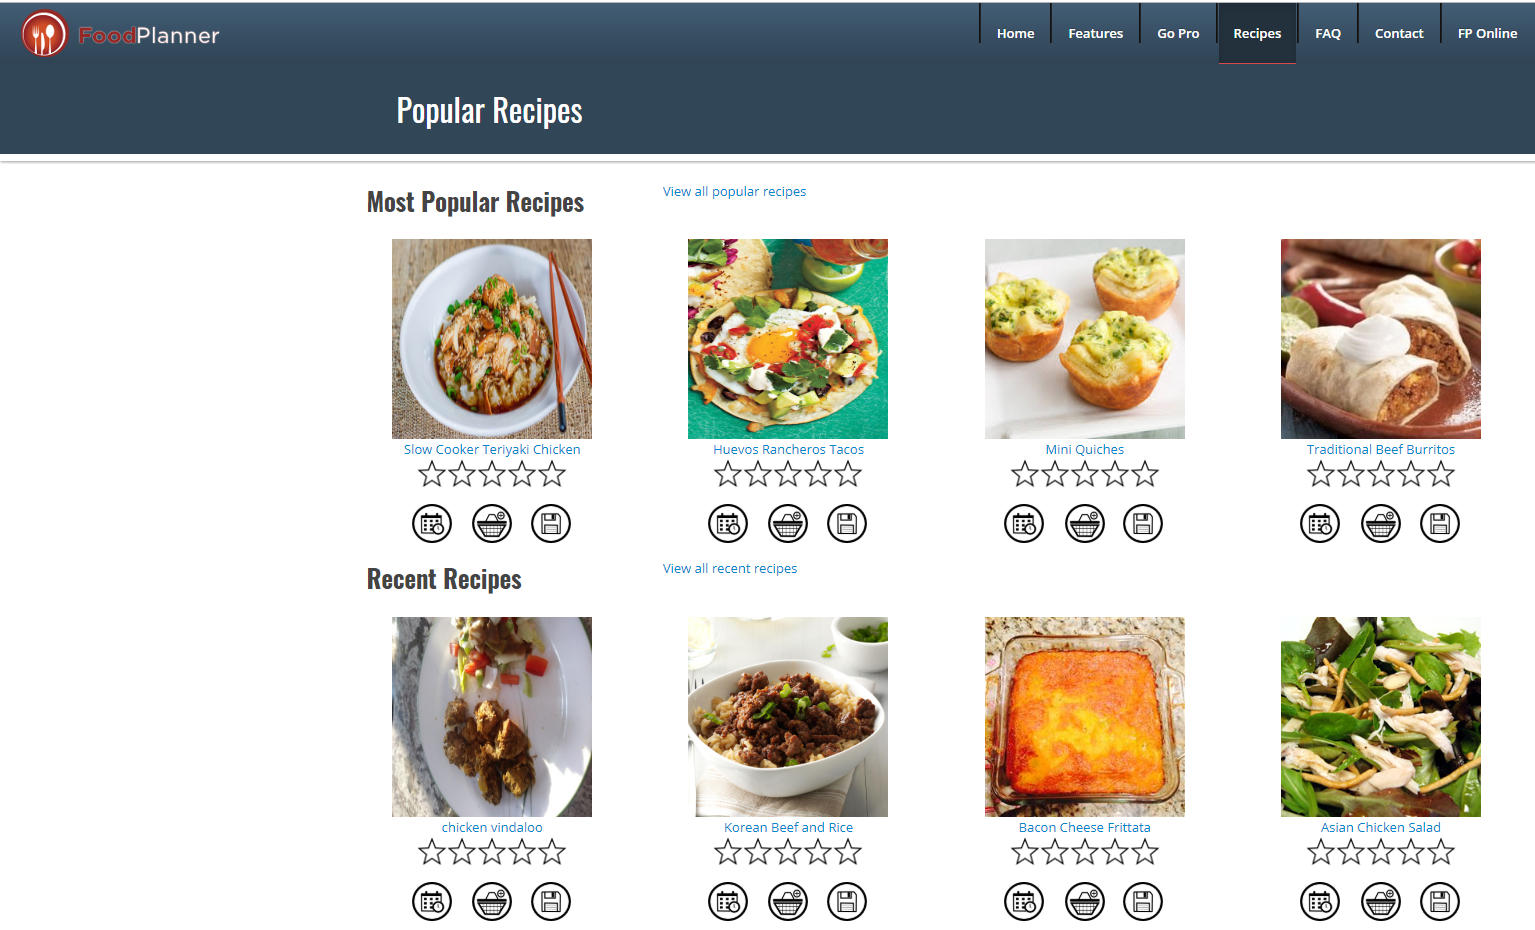
\includegraphics[width=15cm]{Imagenes/FoodPlanner.png}
			\caption{Food Planner}\label{Food Planner}
		\end{figure}
	\end{center}
	Después de una revisión del sistema y un uso del mismo como usuario podemos ver dos problemas principales que intentamos corregir con el planteamiento de nuestro sistema:
	\begin{itemize}
		\item \textbf{Excesivo trabajo necesario por el usuario para poder empezar a utilizar el sistema:} Como ejemplo, al dar de alta un plato, el sistema exige una gran cantidad de datos, a mayores, al no llevar una gestión de ingredientes, cada vez que un nuevo plato utiliza el mismo ingrediente, debemos indicarlo a mano de nuevo sin poder seleccionarlo de nuestros ingredientes registrados. Esto, sumado al hecho de que el usuario debe dar de alta todos los platos que utiliza en su día a día para poder empezar a planificar sus semanas, hace que la mayoría de los sistemas en este ámbito no se utilicen por exigir demasiado por parte del usuario y perder su interés pronto.
		\begin{center}
			\begin{figure}[H]
				\centering
				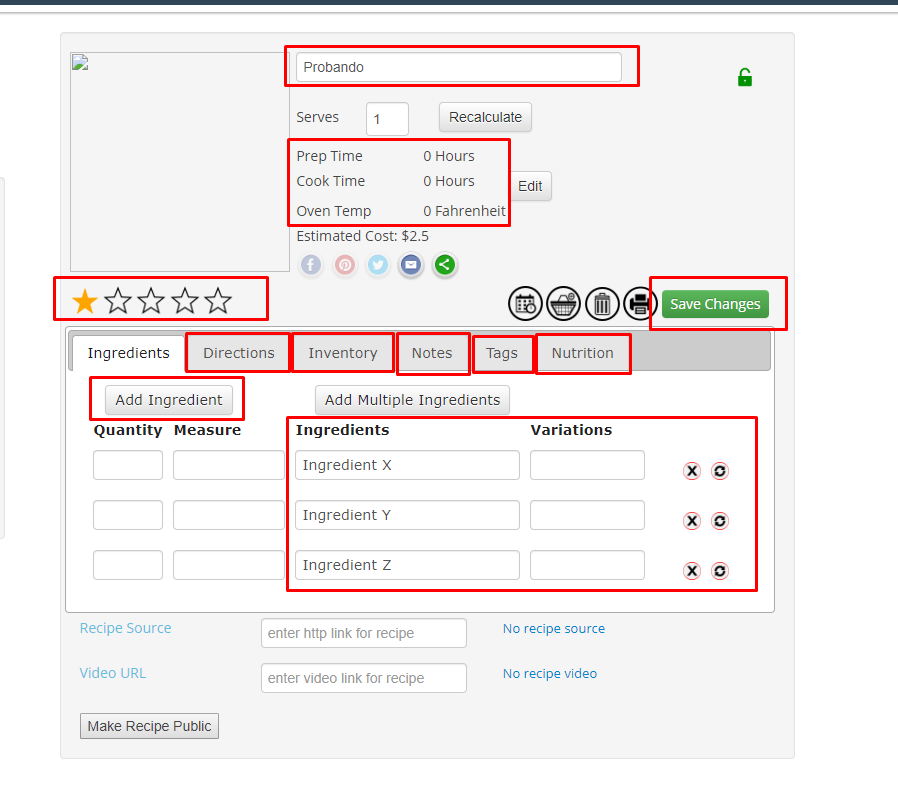
\includegraphics[width=15cm]{Imagenes/FoodPlannerAddRecipe.png}
				\caption{Food Planner Add Recipe}\label{Food Planner Add Recipe}
			\end{figure}
		\end{center}
		\textbf{Solución:} Énfasis en la sencillez en los formularios sin el requerimiento de datos innecesarios y carga de datos base comunes (Ingredientes que utilizará el usuario base en la mayoría de sus platos) en cada registro de nuevos usuarios para evitar trabajo al usuario.
		\item \textbf{Poco énfasis en las características nutricionales de los platos:} En FoodPlanner para obtener las calorías, grasas ... de un plato se requiere indicar una url con la receta de ese plato en páginas concretas seleccionadas, esto es muy laborioso para el usuario ya que para cada plato debe buscar esa receta en dichas páginas y tiene el posible problema de que no exista en esas páginas con lo que el usuario no podría tener datos nutricionales sobre su plato. A mayores, no permite visualizar en el calendario los stats nutricionales del menú actual lo que supone la funcionalidad principal del sistema que planteamos:
		\begin{center}
			\begin{figure}[H]
				\centering
				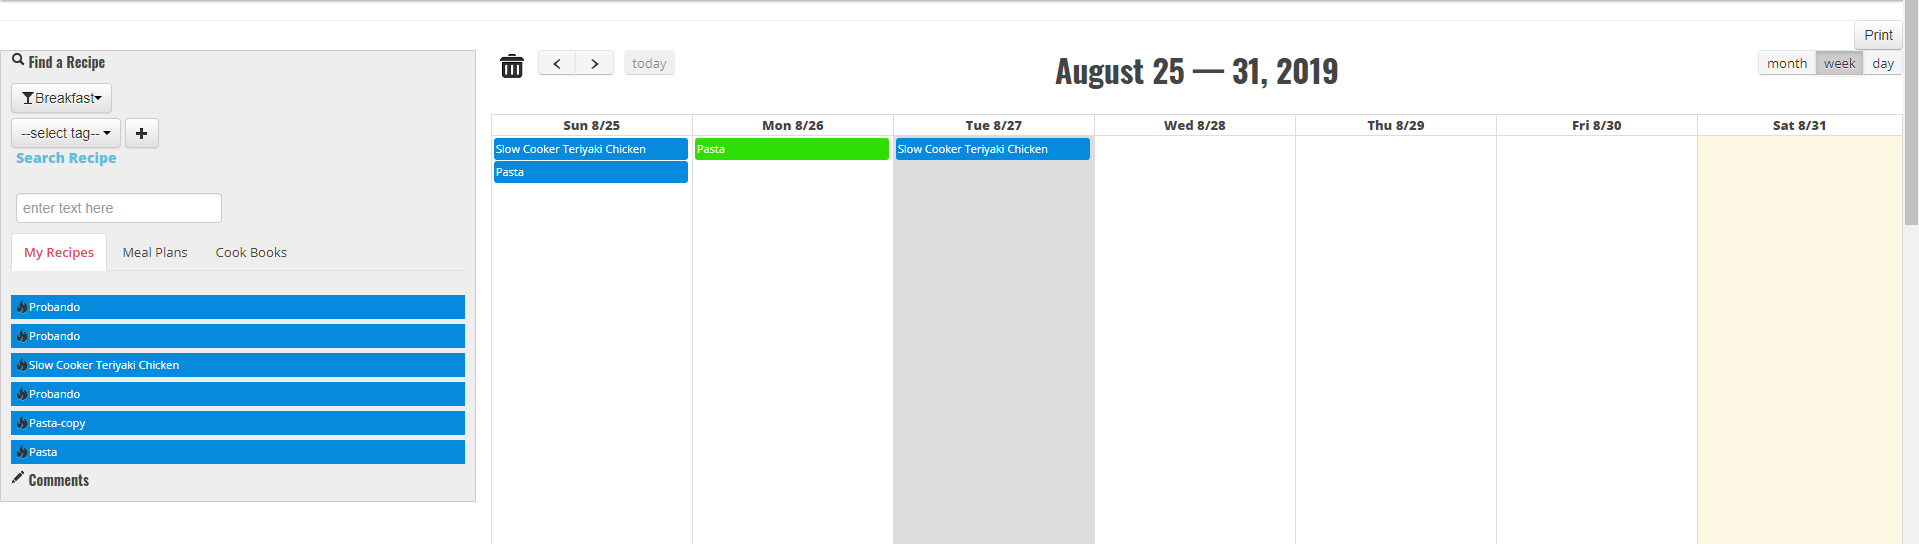
\includegraphics[width=15cm]{Imagenes/FoodPlannerCalendar.png}
				\caption{Food Planner Calendar}\label{Food Planner Calendar}
			\end{figure}
		\end{center}
		\textbf{Solución:} Llamada a un servicio automático para dar valor de stats nutricionales a los ingredientes / platos que registre el usuario pero de forma que sea transparente para él y no le requiera mayor esfuerzo. Énfasis en la visualización de estos stats en todo momento en el menú semanal para dar mayor importancia a los mismos.
	\end{itemize}	
	\section{Eat This Much}
	Así como FoodPlanner es un gestor de recetas que te permite almacenarlas y gestionar sus datos pero que no hace gran énfasis en sus valores nutricionales y su análisis, Eat This Much representa la otra cara de la moneda siendo un sistema que permite indicar las características de la dieta exigida (Calorías, Tipo de dieta, Cantidad de comidas):
	\begin{center}
		\begin{figure}[H]
			\centering
			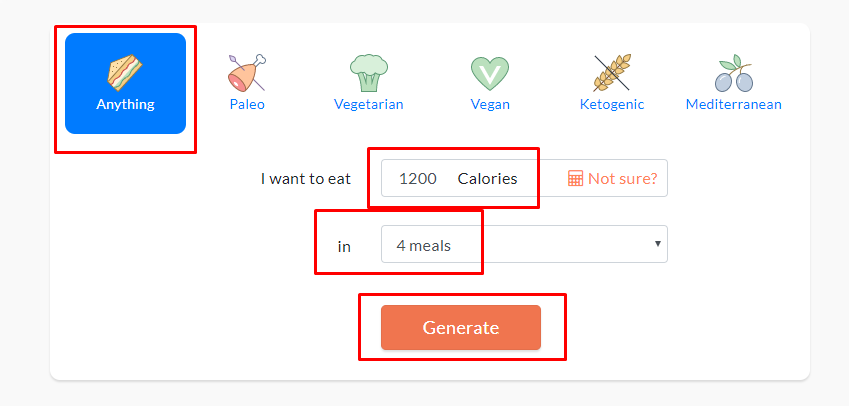
\includegraphics[width=10cm]{Imagenes/EatThisMuchSelection.png}
			\caption{Eat This Much Selection}\label{Eat This Much Selection}
		\end{figure}
	\end{center}
	Y, a partir de esas características, genera automáticamente un menú que las cumple con platos seleccionados por el sistema aleatoriamente:
	\begin{center}
		\begin{figure}[H]
			\centering
			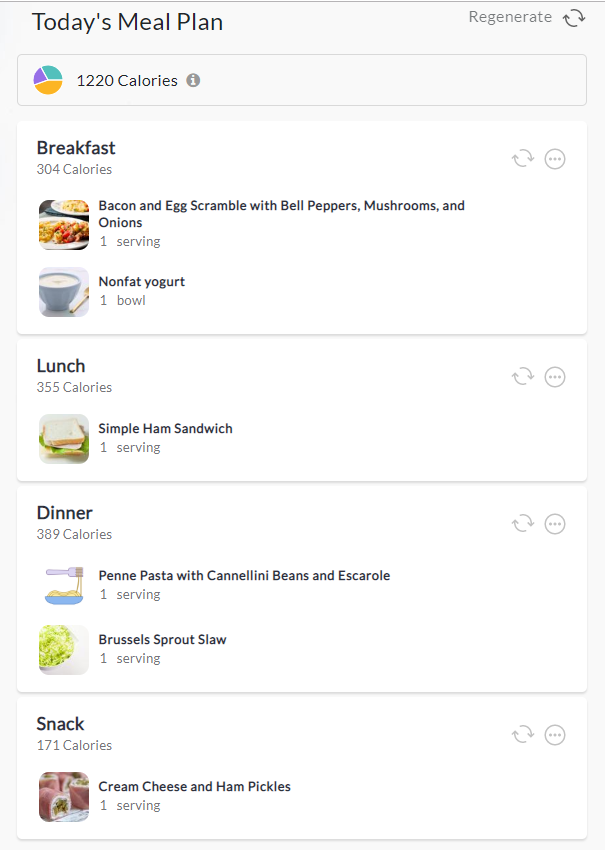
\includegraphics[width=10cm]{Imagenes/EatThisMuchMenu.png}
			\caption{Eat This Much Menu}\label{Eat This Much Menu}
		\end{figure}
	\end{center}
	Al igual que con FoodPlanner es un sistema de software privativo con aplicaciones nativas móviles Android e iOS.
	El \textbf{principal problema} que vemos con este concepto de sistema es que el usuario realmente deja su menú ``a merced'' de la aplicación de forma que puede obtener menús con platos que no sabe cocinar, o bien no le gustan. Aún así, como comentábamos anteriormente, si que vemos una gran ventaja en obtener menús ``aleatorios'' que cumplan las necesidades dietéticas del usuario ya que, al ser aleatorios, evitan rutina y repetición en la dieta del usuario.\\
	Por tanto, la \textbf{principal solución} sería implementar en nuestro sistema un algoritmo de creación de menús válidos pero ÚNICAMENTE con los platos registrados por el usuario, de forma que siga teniendo el control total sobre los platos que aparecerán en sus menús semanales y no aparezcan aquellos no deseados por él.
	\section{Meal-planner}	
	Meal-planner representa un sistema open-source web sin aplicación nativa móvil pero cuyo diseño ha sido adaptado para diferentes pantallas como planteamos en nuestro proyecto.
	En su funcionamiento presenta muchas similitudes con Eat This Much al presentar dos fases, una inicial en la que se hace una encuesta al usuario con la dieta que desea generar (Número de comidas, Seguimiento semanal/diario, Preferencias dietéticas y de salud):
	\begin{center}
		\begin{figure}[H]
			\centering
			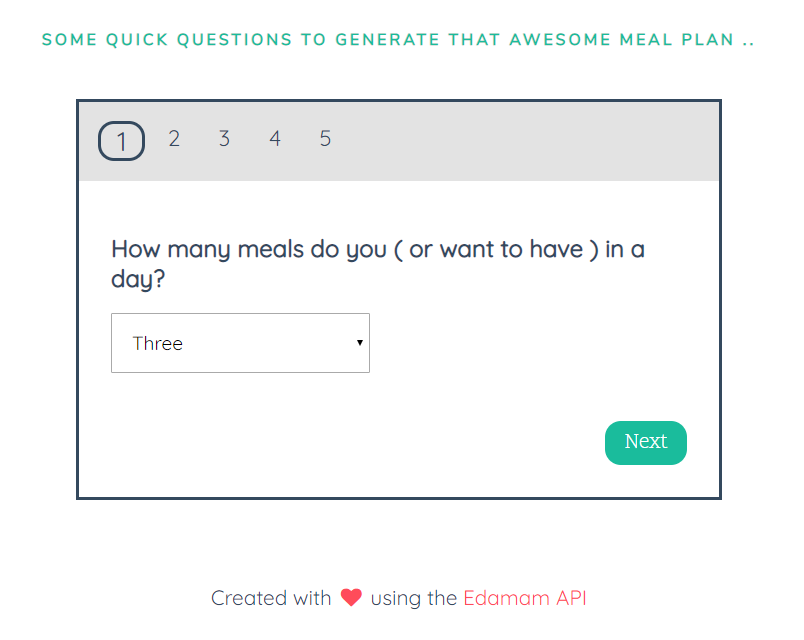
\includegraphics[width=10cm]{Imagenes/MealPlannerSurvey.png}
			\caption{Meal Planner Survey}\label{Meal Planner Survey}
		\end{figure}
	\end{center}
	Una vez completada la encuesta, se genera automáticamente un menú con los días y comidas implicadas.
	\begin{center}
		\begin{figure}[H]
			\centering
			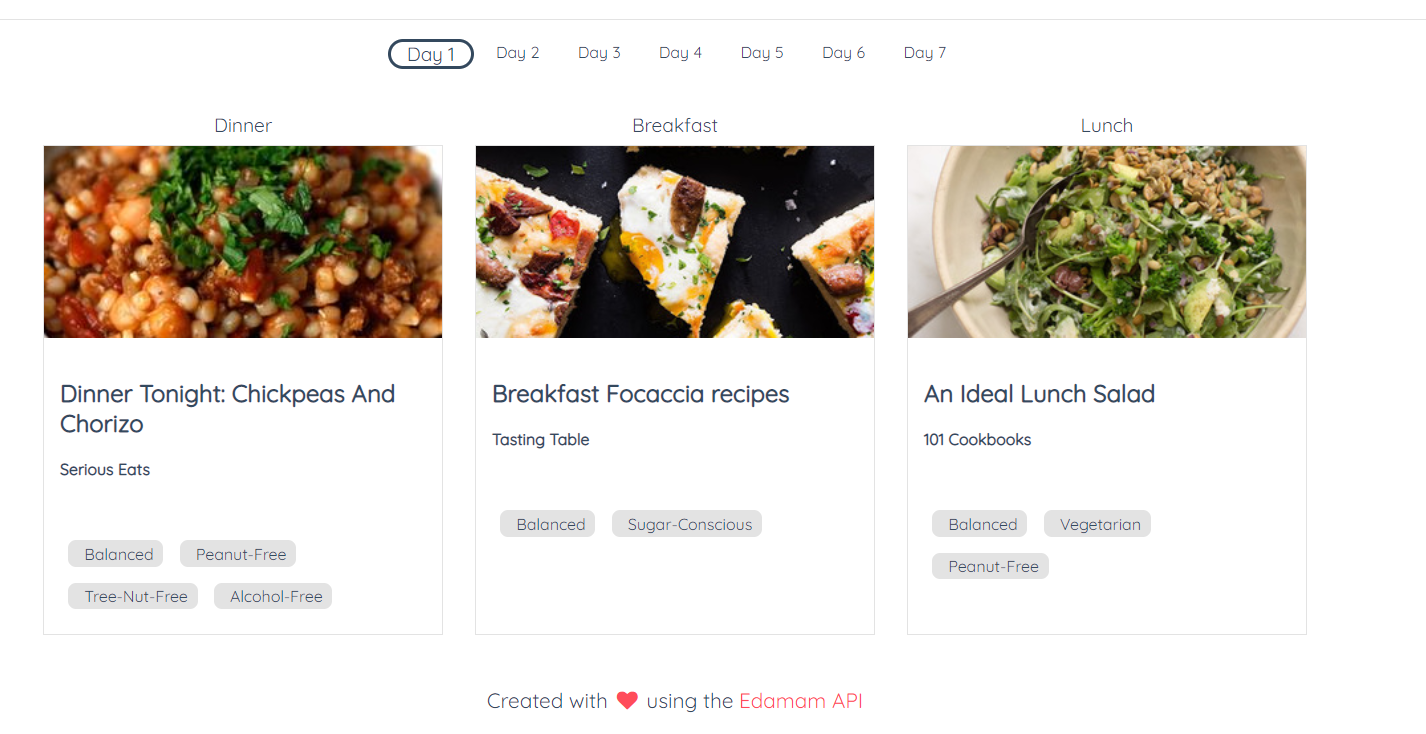
\includegraphics[width=10cm]{Imagenes/MealPlannerMenu.png}
			\caption{Meal Planner Menu}\label{Meal Planner Menu}
		\end{figure}
	\end{center}
	Al igual que en Eat This Much vemos que no se le está dando la posibilidad al usuario de utilizar sus propios platos con lo que podrían requerirse muchas regeneraciones del menú hasta obtener uno de acorde con los gustos y conocimientos culinarios del usuario. Dicha regeneración continua será esfuerzo que al usuario le resultará frustrante. Por otro lado vemos que se deja poco control sobre los valores nutricionales necesarios del usuario.
	\section{What's For Dinner}
	What's For Dinner representa un sistema open-source web responsive sin aplicación móvil de obtención de recetas semanales con un enfoque diferente al visto hasta ahora.
	El usuario dispone de un buscador por el cual puede obtener diferentes resultados de recetas con las palabras clave indicadas:
	\begin{center}
		\begin{figure}[H]
			\centering
			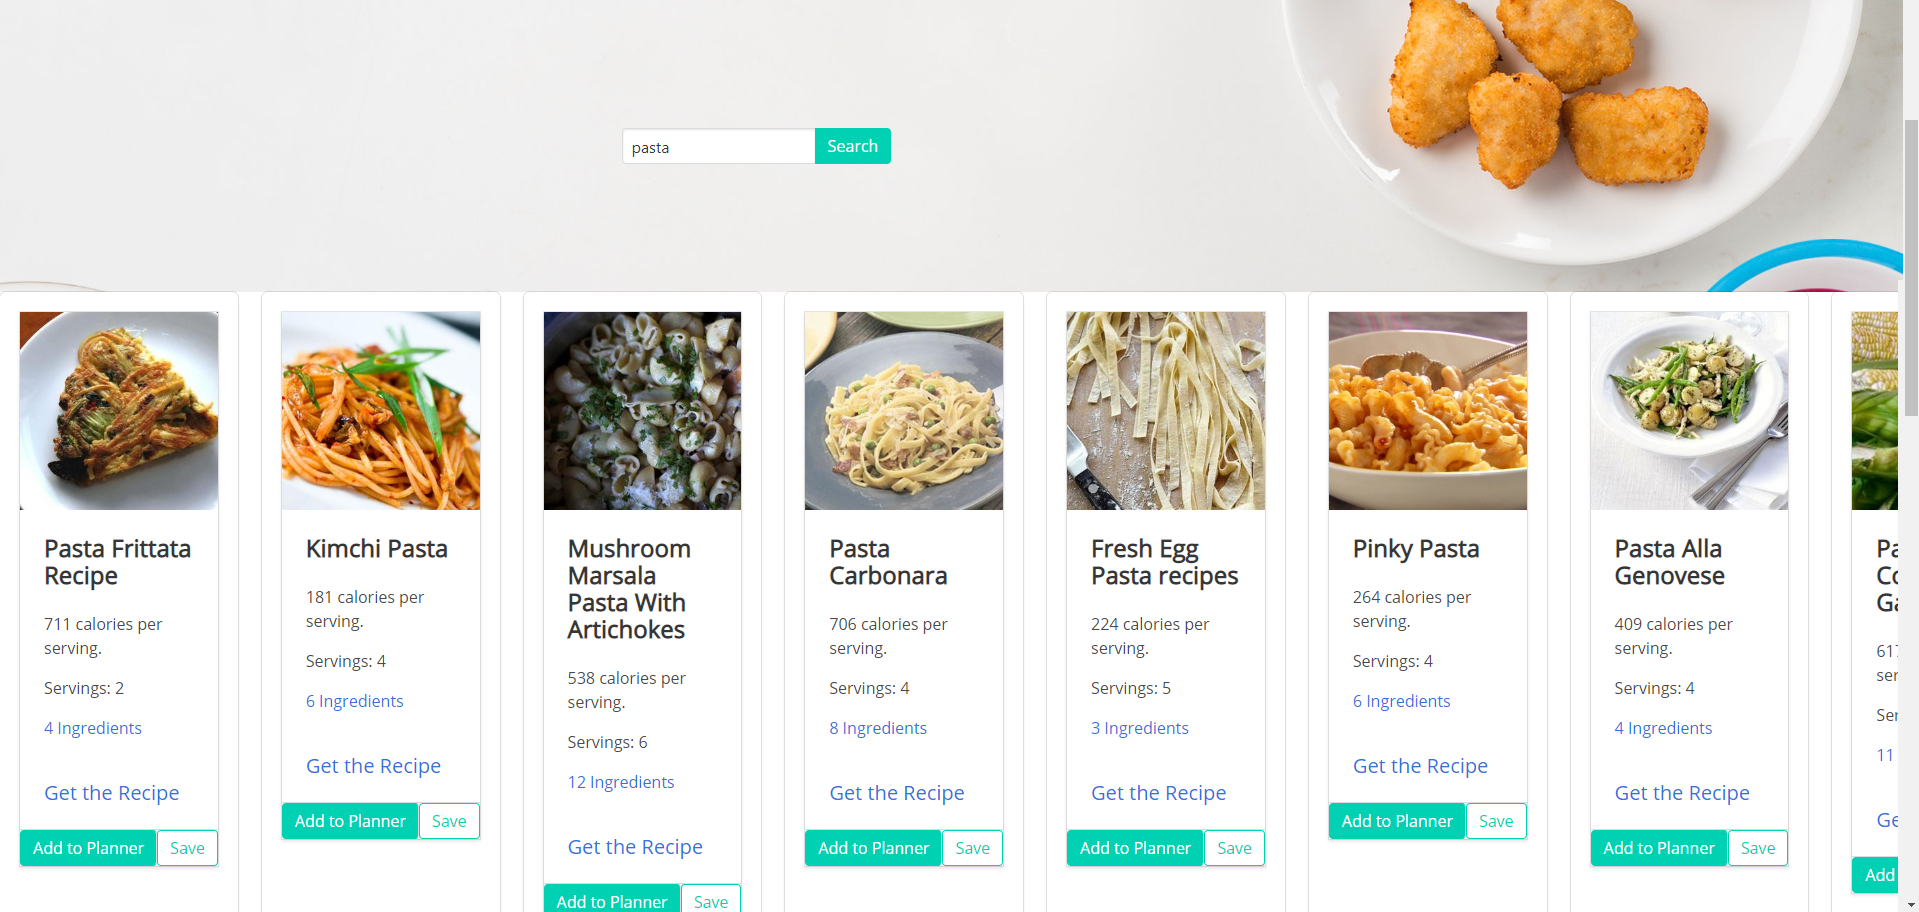
\includegraphics[width=10cm]{Imagenes/WhatsForDinnerSearch.png}
			\caption{What's For Dinner Search}\label{What's For Dinner Search}
		\end{figure}
	\end{center}
	A partir de esos resultados se pueden añadir a alguno de los días de la semana como cena de ese día y se pueden añadir comentarios sobre ese día como por ejemplo en caso de no indicar un plato, poder comentar que se ha pedido a un restaurante fuera ese día:
	\begin{center}
		\begin{figure}[H]
			\centering
			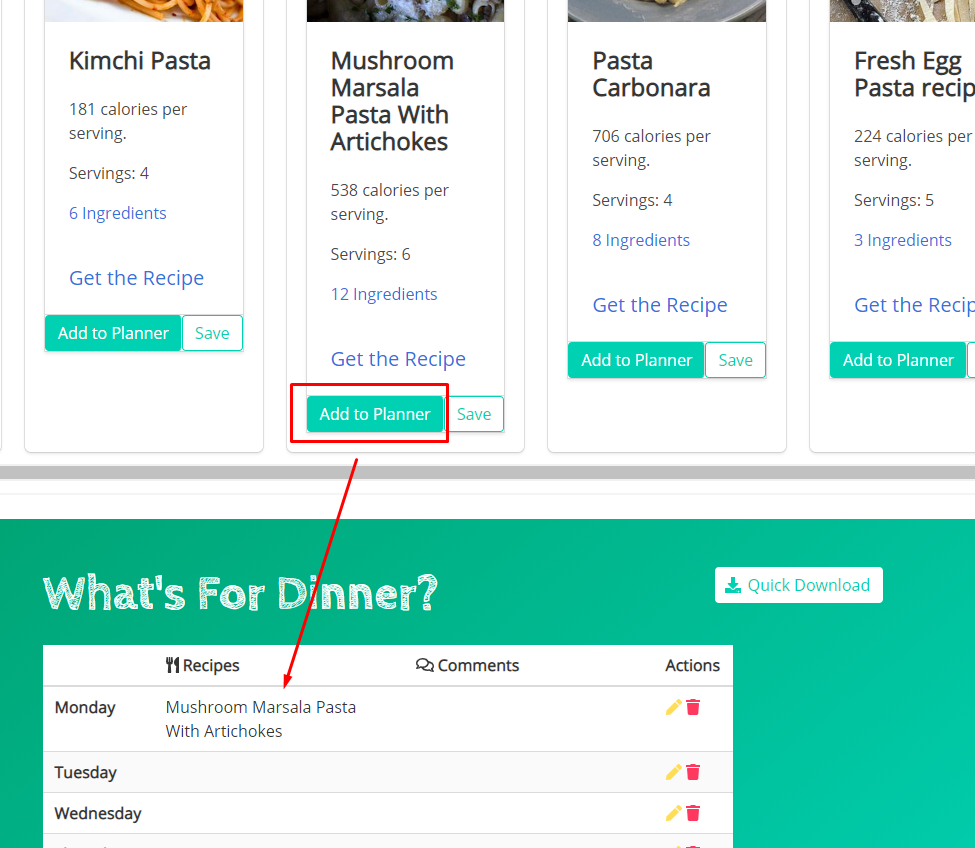
\includegraphics[width=10cm]{Imagenes/WhatsForDinnerMenu.png}
			\caption{What's For Dinner Menu}\label{What's For Dinner Menu}
		\end{figure}
	\end{center}
	A mayores del comentario anterior de no permitir añadir platos nuevos suyos propios al usuario se ve que está un tanto limitado en el sentido de solo permitir planificar una comida por día y solo hacer seguimiento nutricional de las calorías de los platos mostrados en las búsquedas.
	
	\section{Otros}
	Otros sistemas dignos de mención que se han observado en el ámbito nutricional son:
	\begin{itemize}
		\item Allrecipes Dinner Spinner: Es un gestor de recetas web y con aplicaciones móviles que aprende de las preferencias del usuario con énfasis social para la compartición de platos. También recomienda ofertas de ingredientes en tiendas cercanas al usuario.
		\item Veganized: Es una aplicación móvil de gestión y compartición de recetas veganas con funciones para obtener información nutricional de las recetas registradas
		\item Mealime: Es una aplicación web con aplicaciones nativas móviles que permite gestionar diferentes perfiles de personas para las que se quiera cocinar con sus gustos, sus alergias y necesidades alimenticias.
	\end{itemize}
	
	Como resumen del análisis de los sistemas, vemos que deberíamos intentar tomar las fortalezas de todos ellos para formar un sistema que, a mayores de permitir llevar un \textbf{registro de los ingredientes y platos favoritos del usuario}, haga énfasis en la \textbf{sencillez del diseño de los formularios y de la información} siendo este adaptable a pantallas móviles y permita \textbf{generar menús aleatorios acordes a las necesidades dietéticas del usuario}.
	
	\chapter{Base tecnológica}
	En este apartado se describen brevemente las herramientas, frameworks y tecnologías en general utilizadas en el desarrollo de la aplicación. Durante el análisis inicial del proyecto quedó patente el hecho de que una plataforma web era la mejor solución para satisfacer los requisitos planteados, dado que se quería ofrecer un servicio fácilmente accesible a los usuarios. De esta forma la instalación y mantenimiento de la aplicación serían más cómodos para los usuarios (no deben preocuparse por estas cuestiones). Para mejorar el desarrollo y evitar que se acoplen el modelo y la vista, se utiliza el patrón Modelo Vista Controlador llevado hasta el extremo de que el modelo y la vista son artefactos totalmente diferentes lo que facilitará la agregación de una nueva posible vista en el futuro (Aplicaciones nativas móviles, por ejemplo) .
	Para el desarrollo de la aplicación, se opta por utilizar el lenguaje de programación Java EE, puesto que entre otras posee soporte para diversas tecnologías relacionadas con el desarrollo web.
	Para la persistencia de los datos se elige el uso de una base de datos relacional, cuyas características nos ayudan en el control y el correcto almacenamiento de los datos de la aplicación.	
	\section{Lenguajes}
	\subsection{Java SE 8}
	Java Platform, Standard Edition o Java SE, es una colección de APIs del lenguaje de
	programación Java. La plataforma Java es el nombre de un entorno o plataforma de computación
	originaria de Sun Microsystems, capaz de ejecutar aplicaciones desarrolladas usando el
	lenguaje de programación Java u outros lenguajes que compilen a bytecode y un conjunto
	de herramientas de desarrollo. La plataforma es una máquina virtual de proceso nativo, es decir, ejecutable en una plataforma específica, capaz de interpretar y ejecutar instrucciones expresadas en un código binario especial (el bytecode Java), el cual es generado por el compilador del lenguaje Java.\cite{Java}
	La utilización de la versión 8 de java nos facilita la iteración de las colecciones utilizadas mediante el uso de streams y lambdas los cuales limpian el código y mejoran su eficiencia en comportamientos iterativos.
	Se ha tomado Java como lenguaje de programación del servidor por: la sencillez y reusabilidad de la orientación a objetos, la independencia de plataforma que nos aporta Java, la cual es de mayor importancia en un proyecto open-source como el nuestro ya que cualquier posible nuevo contribuidor al proyecto podrá hacerlo sin importar el sistema operativo de su ordenador de trabajo, la inmensa popularidad de java también es una ventaja en este punto ya que será mucho más sencillo encontrar desarrolladores que conozcan este lenguaje.
	\subsection{HTML}
	HTML, siglas de HyperText Markup Language (lenguaje de marcas de
	hipertexto), hace referencia al lenguaje de marcado para la elaboración de páginas
	web. Es un estándar que sirve de referencia para la elaboración de páginas web
	en sus diferentes versiones, define una estructura básica y un código (denominado
	código HTML) para la definición de contenido de una página web, como texto,
	imágenes, vídeos, entre otros. Es un estándar a cargo de la W3C (World Wide
	Web Consortium), organización dedicada a la estandarización de casi todas
	las tecnologías ligadas a la web, sobre todo en lo referente a su escritura e
	interpretación. Se considera el lenguaje web más importante siendo su invención
	crucial en la aparición, desarrollo y expansión de la World Wide Web. Es el
	estándar que se ha impuesto en la visualización de páginas web y es el que todos
	los navegadores actuales han adoptado.\cite{HTML}
	\subsection{CSS}
	CSS es un lenguaje de hojas de estilos creado para controlar el aspecto o presentación de los documentos electrónicos definidos con HTML y XHTML. CSS es la mejor forma de separar los contenidos y su presentación y es imprescindible para crear páginas web complejas.
	
	Separar la definición de los contenidos y la definición de su aspecto presenta numerosas ventajas, ya que obliga a crear documentos HTML/XHTML bien definidos y con significado completo (también llamados "documentos semánticos"). Además, mejora la accesibilidad del documento, reduce la complejidad de su mantenimiento y permite visualizar el mismo documento en infinidad de dispositivos diferentes.
	
	Al crear una página web, se utiliza en primer lugar el lenguaje HTML/XHTML para marcar los contenidos, es decir, para designar la función de cada elemento dentro de la página: párrafo, titular, texto destacado, tabla, lista de elementos, etc.
	
	Una vez creados los contenidos, se utiliza el lenguaje CSS para definir el aspecto de cada elemento: color, tamaño y tipo de letra del texto, separación horizontal y vertical entre elementos, posición de cada elemento dentro de la página, etc.\cite{CSS}
	\section{Frameworks y librerías}
	\subsection{Core}
	\subsubsection{Spring}
	Spring es un “framework” de código abierto, distribuido bajo la licencia Apache
	2.0, para el desarrollo de aplicaciones que proporciona un modelo de config uración y de
	programación ampliado para desarrollos de aplicaciones Java independiente de la
	plataforma. Spring proporciona:
	\begin{itemize}
		\item Un modelo flexible de inyección de dependencias basado en anotaciones o en
		configuraciones XML. Está basado en los principios de Inversión de Control
		(IoC), lo que proporciona un desacoplamiento entre objetos. Esto significa que
		el “framework” llama a procedimientos creados por el programador en lugar de
		ser el programador el que llama a los procedimientos del “framework”.
		\item Soporte avanzado para programación orientada a aspectos, que pretende la
		separación mediante módulos de aspectos comunes aplicándolos de forma
		declarativa, evitando duplicidad de código en diversos elementos. Se utiliza
		sobre todo en gestión de transacciones, seguridad y configuración.
		\item Soporte a declaración, gestión de caché, validación y formato de transacciones.
		\item Abstracción para el trabajo de especificaciones como JDBC, JPA, JMS y JTA.
		\item Soporte de primer nivel para “frameworks” de código abierto comunes como
		Hibernate y Quartz.
		\item Un marco flexible para las construir aplicaciones web MVC y servicios finales.
		\item Y facilidades para la realización de pruebas unitarias, así como pruebas de
		integración.
		
	\end{itemize}
	Spring tiene un diseño modular, como puede verse en la figura, que
	permite cargar solo los módulos necesarios, aligerando el peso de la aplicación.\cite{Spring}
	
	\begin{figure}[H]
		\centering
		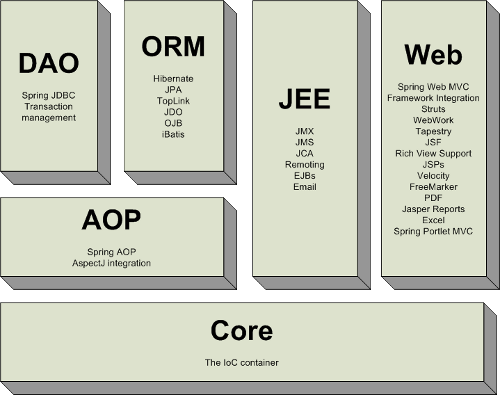
\includegraphics[width=6cm]{Imagenes/spring.png}
		\caption{Spring}\label{spring}
	\end{figure}

	Elegimos Spring como gestor de dependencias ya que nos simplifica mucho el desarrollo encargándose de la definición de consultas básicas en los repositorios mediante Spring Data y de la gestión de transaccionalidad en los métodos de los servicios de negocio. Dispone también de una arquitectura que nos facilitará mucho la aplicación del patrón MVC.

	\subsubsection{Hibernate}	
	Hibernate es una herramienta de Mapeo objeto-relacional (ORM) para la
	plataforma Java que facilita el mapeo de atributos entre una base de datos
	relacional tradicional y el modelo de objetos de una aplicación, mediante archivos
	declarativos (XML) o anotaciones en los beans de las entidades que permiten
	establecer estas relaciones.\\
	\begin{center}
		\begin{figure}[H]
			\centering
			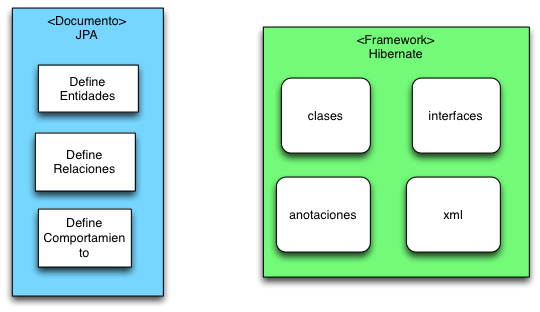
\includegraphics[width=6cm]{Imagenes/hibernate.png}
			\caption{Hibernate}\label{hibernate}
		\end{figure}
	\end{center}

	Elegimos Hibernate ya que en conjunción con Spring Data nos facilita en gran medida la definición de consultas y nos aporta gran escalabilidad por su eficiencia y su arquitectura de caché doble.
	\section{Web}
	\subsubsection{Angular JS}
	AngularJS (comúnmente llamado Angular.js o AngularJS 1), es un framework de javascript de código abierto, mantenido por google, que se utiliza para crear y mantener aplicaciones web de una sola página. Su objetivo es aumentar las aplicaciones basadas en navegador con capacidad de Modelo Vista Controlador (MVC), en un esfuerzo para hacer que el desarrollo y las pruebas sean más fáciles.
	
	La biblioteca lee el HTML que contiene atributos de las etiquetas personalizadas adicionales, entonces obedece a las directivas de los atributos personalizados, y une las piezas de entrada o salida de la página a un modelo representado por las variables estándar de JavaScript. Los valores de las variables de JavaScript se pueden configurar manualmente, o recuperados de los recursos JSON estáticos o dinámicos.
	
	AngularJS se puede combinar con el entorno en tiempo de ejecución Node.js, el framework para servidor Express.js y la base de datos MongoDB para formar el conjunto MEAN.\\
	
	Elegimos AngularJS como framework de frontend a mayores de por la motivación de aprendizaje tecnológico que se ha comentado, nos da la oportunidad de crear una Single Page Application cuya rapidez mejora mucho la experiencia de usuario. El código desarrollado en AngularJS será muy limpio y mantenible y permite emplear pruebas unitarias.
	
	\begin{center}
		\begin{figure}[H]
			\centering
			
\includegraphics[width=10cm]{Imagenes/angularjs.jpg}
			\caption{Angular JS}\label{angularjs}
		\end{figure}
	\end{center}
	\subsubsection{Bootstrap}    
	Twitter Bootstrap es un framework o conjunto de herramientas de software
	libre para diseño de sitios y aplicaciones web. Contiene plantillas de diseño con
	tipografía, formularios, botones, cuadros, menús de navegación y otros elementos
	de diseño basado en HTML y CSS, así como extensiones de JavaScript opcionales
	adicionales.
	
	Elegimos integrar AngularJS con Bootstrap porque con una configuración mínima obtenemos un estilo muy elegante para nuestra web que es compatible con todos los navegadores.
	\subsection{Pruebas}
	\subsubsection{JUnit}
	JUnit es un conjunto de bibliotecas utilizadas en programación para hacer
	pruebas unitarias y de integración de aplicaciones Java.
	JUnit es un conjunto de clases (framework) que permite realizar la ejecución
	de clases Java de manera controlada, para poder evaluar si el funcionamiento de
	cada uno de los métodos de la clase se comporta como se espera. Es decir, en
	función de algún valor de entrada se evalúa el valor de retorno esperado; si la
	ejecución cumple con la especificación, entonces JUnit devolvería que el método
	de la clase pasó exitosamente la prueba; en caso de que el valor esperado sea
	diferente al que devolvió el método durante la ejecución, JUnit devolvería un fallo
	en el método correspondiente.
	JUnit es también un medio para realizar las pruebas de regresión, necesarias
	cuando una parte del código ha sido modificado y se desea ver que el nuevo código
	cumple con los requerimientos anteriores y que no se ha alterado su funcionalidad
	después de la nueva modificación.\cite{JUnit}
	Elegimos JUnit como framework de pruebas unitarias ya que supone un estandard de testeo Java que está soportado por la gran mayoría de los IDEs y que es conocido por la gran parte de los desarrolladores Java. A mayores con JUnit podemos desarrollar rápidamente y mantener una gran suite de casos de prueba unitarios.
	\subsubsection{Mockito}
	Mockito es un framework open source para Java desarrollado bajo la licencia de MIT. El framework permite la creación the objetos de pruebas en tests unitarios automáticos para permitir test-driven development o behavior-driven development. Elegimos Mockito ya que nos agiliza la definición de nuevos casos de prueba unitarios al permitirnos mockear la información obtenida de componentes externos a los del método probado.
	\subsubsection{Eclemma}	
	EclEmma es una herramienta de cobertura de código Java para Eclipse, disponible para la Licencia Pública de Eclipse. Trae el análisis de cobertura de código directamente al entorno de Eclipse:\cite{Eclemma}		
	\begin{itemize}
		\item Rápido ciclo de desarrollo/prueba: Arranca desde dentro del entorno como las ejecuciones de los tests de JUnit que pueden ser analizados directamente para cobertura de código.
		\item Intenso análisis de cobertura: Los resultados de cobertura son resumidos inmediatamente y resaltados en los editores de código fuente Java.
		\item No invasivo: EclEmma no requiere modificaciones en tus proyectos o realizar ningún otro ajuste.
	\end{itemize}	
	\subsection{Protocolos}
	\section{Hypertext Transfer Protocol o HTTP}
	Es el protocolo de comunicación que permite las transferencias de información en la World Wide Web. HTTP fue desarrollado por el World Wide Web Consortium y la Internet Engineering Task Force, colaboración que culminó en 1999 con la publicación de una serie de RFC, el más importante de ellos es el RFC 2616 que especifica la versión 1.1. HTTP define la sintaxis y la semántica que utilizan los elementos de software de la arquitectura web (clientes, servidores,proxies) para comunicarse. HTTP es un protocolo sin estado, es decir, no guarda ninguna información sobre conexiones anteriores. El desarrollo de aplicaciones web necesita frecuentemente mantener estado. Para esto se usan las cookies, que es información que un servidor puede almacenar en el sistema cliente. Esto le permite a las aplicaciones web instituir la noción de "sesión", y también permite rastrear usuarios ya que las cookies pueden guardarse en el cliente por tiempo indeterminado.
	\subsection{Herramientas de Desarrollo}
	\subsubsection{Maven}
	Maven es una herramienta de software para la gestión y construcción de
	proyectos Java. Es similar en funcionalidad a Apache Ant, pero tiene un modelo
	de configuración de construcción más simple, basado en un formato XML.
	Maven utiliza un Project Object Model (POM) para describir el proyecto de
	software a construir, sus dependencias de otros módulos y componentes externos,
	y el orden de construcción de los elementos. Viene con objetivos predefinidos para
	realizar ciertas tareas claramente definidas, como la compilación del código y su
	empaquetado.
	Para desarrollar esta aplicación se ha optado por realizar la implementación con el lenguaje de programación Java haciendo uso del IDE Eclipse EE como entorno de desarrollo. Se ha tomado esta decisión puesto que se tiene experiencia previa de su uso y por la gran cantidad de manuales y soporte disponible. Este proyecto ha sido desarrollado sobre un sistema Windows.
	Eclipse es una comunidad de código abierto cuyos proyectos se centran en la construcción de una plataforma de desarrollo extensible, que facilita la gestión de los tiempos de ejecución y de los marcos de aplicación para la construcción, despliegue y gestión de software a través de todo el ciclo de vida del software. Eclipse, además de un IDE, entorno de desarrollo de aplicaciones enriquecidas, es una comunidad que proporciona herramientas y plugins para ayudar al desarrollo de software \cite{Maven}.
	Elegimos Maven como gestor de dependencias por su buena integración con el Framework de Spring como dependencia así como por su sencillez de definición a través de los diferentes POM.xml de la aplicación. Maven también nos facilita la búsqueda de problemas en el sistema al permitirnos debuggear las clases de las librerías importadas.
	\subsection{Sistemas de Gestión de Bases de Datos}
	\subsubsection{MySQL}
	MySQL es un sistema de gestión de base de datos relacional, que está disponible
	bajo licencia GPL y que tiene como características principales el soporte multitarea,
	mediante hilos del núcleo; el soporte de gran cantidad de datos; soporte multiusuario,
	con gestión de seguridad mediante contraseñas, privilegios y cifrado; y que está
	disponible sobre múltiples plataformas.\cite{MySQL}
	Elegimos MySQL como base de datos por su gran seguridad en la gestión de transacciones, su alta eficiencia y escalabilidad flexible. Su naturaleza opensource entra dentro de nuestra filosofía de proyecto.
	\subsection{Herramientas de apoyo}
	\begin{itemize}
		\item Trello: Se trata de una aplicación web para la gestión de proyectos de forma colaborativa, la cual se compone de tableros con listas de tareas compuestas de una manera muy intuitiva. Permite tener varias listas de tareas a modo de columnas, y arrastrar tareas de una a otra (por ejemplo pasar una tarea de la lista en progreso a finalizado). Al tratarse de una herramienta colaborativa, permite que varias personas puedan consultar y utilizar el mismo tablero, asignando tareas y añadiendo comentarios.
		\item Navegadores: Dado que el proyecto consiste en el desarrollo de una aplicación web, se han utilizado diferentes navegadores durante el desarrollo para realizar las pruebas de todas las funcionalidades. Los navegadores utilizados han sido Firefox, Chrome, Opera Browser e Internet Explorer.
		\item TexStudio: TeXstudio es un entorno de escritura integrado para crear documentos LaTeX. Su objetivo es hacer que escribir LaTeX sea lo más fácil y cómodo posible. Por lo tanto, TeXstudio tiene varias características tales como destacado de sintaxis, visualizador integrado, comprobador de referencias y varios asistentes. 
		Texstudio es de código libre y está disponible para todos los grandes sistemas operativos. Texstudio se ha separado de Texmaker en 2009, debido a los procesos de desarrollo no abiertos de Texmaker y a diferencias filosofías referentes a configurabilidad y características. Originalmente fue llamado TeXmakerX porque empezó como un pequeño conjunto de extensiones de Texmaker con la esperanza de que se integrarían en Texmaker algún día. Mientras que en algunos puntos aún se puede ver que Texstudio se originó de Texmaker, cambios significativos en características y en el código base lo han convertido en un programa completamente independiente. 
		TeXstudio funciona en Windows, Unix/Linux, BSD y Mac OS X. Está licenciado bajo GPL v2. Al ser de código libre, se puede utilizar y modificar a gusto.\cite{TexStudio}
		\item Git\cite{Git}:
		Git es un sistema de control de versiones distribuido gratuito y de código abierto diseñado para manejar todos los proyectos, pequeños a muy grandes con rapidez y eficiencia.
		
		Git es fácil de aprender y se consigue un rendimiento increíblemente rápido con poco trabajo. Representa una gran mejora con respecto a herramientas de tipo SCM tales como Subversion, CVS, Perforce y ClearCase con características como ramificación local sencilla, áreas de almacenamiento convenientes y múltiples flujos de trabajo.
		Con git se pueden realizar tareas como las siguientes:
		\begin{itemize}
			\item Cambio de contexto sin fricción.
			\item Ramificación basadas en roles.
			\item Flujo de trabajo basado en características.
			\item Experimentación desechable.
		\end{itemize}
		\begin{figure}[H]
			\centering
			
\includegraphics[width=4cm]{Imagenes/git.png}
			\caption{Git}\label{git}
		\end{figure}
	
		Gestionamos el proyecto en un github público que puede ser accedido por cualquier colaborador interesado.
		
		\item \LaTeX{}:
		LaTex es un sistema de composición de textos, orientado especialmente a la creación de libros, documentos científicos y técnicos que contengan fórmulas matemáticas. Es el sistema empleado para la realización de toda la documentación del proyecto (incluyendo esta memoria). Consiste en un lenguaje que permite a la persona que escribe el documento no tener que preocuparse del formato.\cite{Latex}
		Elegimos LaTeX para generar la memoria porque nos facilita el formateado del documento y tiene una mayor potencia de configuración que un editor de texto básico como Word.
		
		\item UML:
		UML te ayuda a especificar, visualizar y documentar modelos de sistemas software, incluyendo su estructura y  diseño, de una forma que cumple todos esos requisitos. (UML puede ser empleado para modelado de negocios y modelado de otros sistemas no software también) Usando cualquiera del gran número de herramientas basadas en UML en el mercado es posible analizar los requisitos de las futuras aplicaciones y diseñar soluciones que los cumplan, representando los resultados usando los trece tipos de estándares de diagramas de UML 2.0 .
		Es posible modelar prácticamente cualquier tipo de aplicación, funcionando en cualquier tipo y combinación de hardware, sistema operativo, lenguaje de programación, y red, en UML. Su flexibilidad permite al usuario modelar aplicaciones distribuidas que utilizan casi cualquier middleware en el mercado. Formado a partir de conceptos fundamentales de Orientación a Objetos incluyendo class y operación, se adecúa con facilidad a lengujaes y entornos orientados a objetos tales como C++, Java, y el reciente C Sharp, pero también puede ser empleado para modelar aplicaciones no orientadas a objetos, por ejemplo, Fortran, VB, o COBOL. Perfiles UML facilitan el modelado de sistemas Transaccionales, de Tiempo Real y Tolerantes a Fallos de una manera natural.\cite{UML}
		
	\end{itemize} 
	\chapter{Metodología y Planificación}
	\section{Metodología e Iteraciones}
	Para que un proyecto software se realice correctamente es necesario seguir una metodología adecuada a su tamaño y propósito. La metodología utilizada para desarrollar este proyecto ha sido Scrum.
	\subsection{Scrum}
	Scrum es un marco de trabajo para desarrollo ágil de software.\\
	Es un proceso en el que se aplican de manera regular un conjunto de buenas prácticas para trabajar colaborativamente, en equipo y obtener el mejor resultado posible de proyectos, caracterizado por:
	\begin{itemize}
		\item Adoptar una estrategia de desarrollo incremental, en lugar de la planificación y ejecución completa del producto.
		\item Basar la calidad del resultado más en el conocimiento tácito de las personas en equipos auto organizados, que en la calidad de los procesos empleados.
		\item Solapar las diferentes fases del desarrollo, en lugar de realizar una tras otra en un ciclo secuencial o en cascada.
	\end{itemize}	
	\begin{figure}[H]
		\centering
		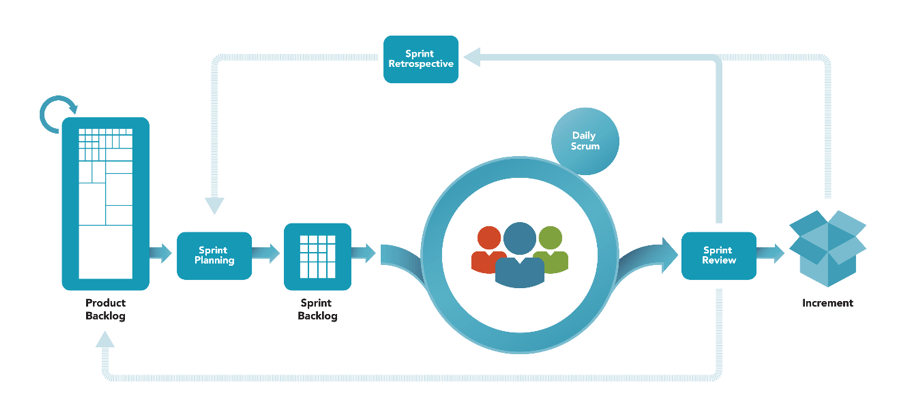
\includegraphics[width=15cm]{Imagenes/Scrum.png}
		\caption{Scrum}\label{Scrum}
	\end{figure}
	Se toma la decisión de esta metodología ya que con el desarrollo iterativo nos permitirá adaptarnos a los posibles cambios de alcance que se encuentren en el desarrollo del proyecto. También nos permitirá hacer un seguimiento muy cercano al avance del proyecto permitiéndonos corregir el enfoque en caso de estarnos desviando del camino correcto.
	En la aplicación de Scrum en nuestro proyecto hemos realizado Sprints semanales con una reunión a su final con los objetivos de una Sprint Review, para analizar los avances realizados en el sprint y el Sprint Planning de la siguiente semana para revisar el enfoque y verificar cuánta capacidad se tendrá en el sprint para avanzar en las historias de usuario. Para la priorización de las historias de usuario se han organizado de forma que en los dos primeros sprints de desarrollo tengamos un MVP del sistema con interacción entre el backend y el frontend y, a partir de este MVP, hemos ido añadiendo funcionalidades adicionales que tengamos estimadas como aquellas que más valor aportan a nuestro sistema.
	\section{Planificación y análisis de costes}
	\subsection{Análisis de viabilidad}
	Ya que vemos que existen muchos otros sistemas similares al nuestro, realizamos encuestas con diferentes potenciales usuarios de nuestro sistema y les explicamos el enfoque que diferenciaría al nuestro y que supone una ventaja con respecto al resto, el seguimiento de los stats nutricionales de los menús semanales y el diseño minimalista y user friendly de nuestras interfaces. Tras recibir resultados positivos de todas las personas con las que hemos hablado, realizamos una planificación del trabajo necesario para implementar el sistema para poder estimar el esfuerzo requerido y ver si sería una cantidad manejable.
	\subsection{Planificación}
	El objetivo de la división del trabajo es poder organizar estas tareas en Sprints.\\
	Sprint es el nombre que va a recibir cada uno de los ciclos o iteraciones que vamos a tener dentro de dentro de nuestro proyecto.\\	
	Nos van a permitir tener un ritmo de trabajo con un tiempo prefijado, siendo la duración de nuestro Sprint una semana. Teniendo sprints cortos tenemos una mayor adaptabilidad al cambio y un seguimiento más cercano del avance.	En cada Sprint o cada ciclo de trabajo lo que vamos a conseguir es lo que se denomina un entregable o incremento del producto, que aporte valor al cliente.
	En esta división obtenemos la siguiente lista de historias de usuario ordenadas por prioridad, descripción de una funcionalidad que debe incorporar un sistema de software, y cuya implementación aporta valor al cliente:
	\begin{itemize}
		\item HU01-Dar de alta un ingrediente
		\item HU02-Dar de alta un plato
		\item HU03-Visión semanal de menú
		\item HU04-Generación de lista de la compra
		\item HU05-Gestión de usuarios
		\item HU06-Configuraciones de usuario: dietéticas y de preferencias
		\item HU07-Análisis dietético dinámico de menú
		\item HU08-Integración con WS de características nutricionales para estimación de ingredientes
		\item HU09-Integración con supermercados para estimar un precio de la compra
		\item HU10-Recetario
		\item HU11-Generación aleatoria de menú
		\item HU12-Generación de menú de acorde a las características dietéticas
		\item HU13-Compartición por redes sociales
		\item HU14-Énfasis en UX y diferentes tamaños de pantalla
		\item HU15-Machine Learning para sugerir platos nuevos
	\end{itemize}
	\subsubsection{Planificación previa}
	Este proyecto cuenta principalmente con dos recursos, un Analista/Programador que es el creador de esta memoria, y un Jefe de Proyecto que es el director del mismo Juan José Sánchez. Para ambos recursos un día de trabajo consta de 8 horas. El desarrollador ha llevado una jornada de cinco días de trabajo semanales mientras que el Jefe de Proyecto ha realizado un día semanal de feedback y revisión del estado.
	\subsubsection{Sprints}
	Realizaremos el desarrollo del proyecto en 15 semanas con lo que tendremos 15 sprints. Realizamos la asignación de las historias de usuario a cada uno de los sprints balanceándolas de forma que todos los sprints tengan la misma carga de trabajo. Tenemos una serie de sprints iniciales y finales en los que se realizan una serie de tareas no relacionadas con el desarrollo directo pero necesarias para nuestro sistema.
	\begin{itemize}
		\item Sprint 1 : Estudio del dominio nutricional y de sus necesidades de automatización
		\item Sprint 2 : Estudio del arte y análisis de competidores con sus ventajas y debilidades
		\item Sprint 3 : Formación en Angular y demás tecnologías seleccionadas
		\item Sprint 4 : HU01-Dar de alta un ingrediente y HU02-Dar de alta un plato
		\item Sprint 5 : HU03-Visión semanal de menú
		\item Sprint 6 : HU04-Generación de lista de la compra
		\item Sprint 7 : HU05-Gestión de usuarios y HU06-Configuraciones de usuario: dietéticas y de preferencias
		\item Sprint 8 : HU07-Análisis dietético dinámico de menú
		\item Sprint 9 : HU08-Integración con WS de características nutricionales para estimación de ingredientes
		\item Sprint 10 : HU09-Integración con supermercados para estimar un precio de la compra
		\item Sprint 11 : HU10-Recetario
		\item Sprint 12 : HU11-Generación aleatoria de menú y HU12-Generación de menú de acorde a las características dietéticas y HU13-Compartición por redes sociales
		\item Sprint 13 : HU14-Énfasis en UX y diferentes tamaños de pantalla y HU15-Machine Learning para sugerir platos nuevos
		\item Sprint 14 : Refactorización y maduración de interfaz
		\item Sprint 15 : Pruebas de integración y de usuario sobre el sistema 
	\end{itemize}
	
	
	\begin{tabular}{| p{5cm} | p{3cm} | p{3cm} | p{3cm} |}
	\hline
	\textbf{Recurso} & \textbf{Nome} & \textbf{Coste/hora} & \textbf{Coste/día}
	\\ \hline
	{Analista/Programador} & {Elías Ferreiro Borreiros} & {30\euro} & {240\euro}
	\\ \hline
	{Jefe de Proyecto} & {Juan José Sánchez} & {50\euro} & {400\euro}
	\\ \hline
		
	\end{tabular}		
	
	\captionof{table}{Recursos empleados en el proyecto}
	
	\begin{tabular}{|p{5cm} | p{2cm} | p{2cm} | p{2cm} | p{2cm} |}
		
		\hline
		\textbf{Recurso} & \textbf{Sprints} & \textbf{Horas / Sprint} & \textbf{Coste / Sprint} & \textbf{Coste total (\euro)}
		\\ \hline
		\textbf{Analista/Programador} & 15 & 40 & 1200\euro  & 18000\euro
		\\ \hline
		\textbf{Xefe de Proxecto} & 15 & 8 & 400\euro & 6000\euro		
		\\ \hline
		\textbf{TOTAL} & & & & 24000\euro
		\\ \hline
	\end{tabular}
	
	\captionof{table}{Costes totales siguiendo la planificación}

	\chapter{Análisis}
	\section{Introducción y Objetivos}
	En esta fase se realiza un estudio de viabilidad del proyecto y se determinan las especificaciones que debe cumplir el sistema. Este análisis de requisitos implica encontrar todas las exigencias y necesidades, así como las restricciones que debe contemplar el sistema. La información obtenida durante esta actividad puede verse en los diagramas casos de uso que se han detallado. También se obtiene un diagrama entidad-relación con el modelado de los datos necesario para almacenar la información.
	\section{Requisitos del sistema}
	En esta sección analizaremos los aspectos que debe cumplimentar nuestro sistema:
	
	El objetivo de este proyecto es el desarrollar un sistema que permita al usuario planificar sus comidas semanalmente haciendo un seguimiento cercano de las características nutricionales de esas comidas y permitiendo al usuario indicar un límite en esos stats que podrá verificar que cumple con su planificación semanal.
	A mayores, se llevará una gestión de ingredientes y platos registrados y mantenidos por el usuario. Con los platos que da de alta el usuario se podrán montar menús semanales sobre los que hacer seguimiento.
	Estos menús deben permitir generarse automáticamente o bien de forma aleatoria o bien de forma válida sin violar los límites indicados por el usuario. A partir del menú debemos poder obtener su lista de la compra para saber que ingredientes comprar para poder cocinarlo a lo largo de la semana, en esta lista deberíamos tener una estimación del precio que correspondería a su compra completa.
	Tendremos también una gestión de plantillas de menú para facilitar la generación de nuevos menús a través de menús previos guardados como plantillas que hayan sido de gusto para el usuario.
	
	Como requisitos técnicos no funcionales debemos hacer énfasis sobre la sencillez del diseño de los formularios para evitar inundar al usuario con gran cantidad de campos a cubrir en el alta de nuevos ingredientes y / o platos y deberíamos permitir un buen diseño visual en diferentes tamaños de pantalla al no disponer de una aplicación nativa móvil como forma de facilitar la usabilidad del usuario desde cualquier plataforma que tenga disponible. Teniendo en cuenta que esperamos que el número de usuarios sea elevado al ser tan grande el grupo demográfico correspondiente al usuario base con lo que se debe hacer énfasis en la escalabilidad del sistema y el mantenimiento de la eficiencia.
	\section{Actores}
	\begin{itemize}
		\item Usuario: Representa la persona que utiliza nuestro sistema para recibir valor de sus funcionalidades.
		\item Sistema Estimador Nutricional (SEN): Representa al sistema externo que, al recibir la orden de nuestro sistema, estimará los valores nutricionales de un ingrediente a partir de su nombre.
		\item Sistema Scrapeador de Supermercado (SSS): Representa al sistema externo que, al recibir la orden de nuestro sistema, consultará la página de un supermercado para obtener su catálogo y sus precios.
	\end{itemize}
	\section{Casos de Uso}
	\subsection{Casos de uso Usuario}
	\subsubsection{CU-001-Registro}
	Proceso de creación de la cuenta del usuario en la aplicación. Se solicitará el email, el nombre, los apellidos y la contraseña.
	Se comprobará que el usuario introducido no existiera previamente en la aplicación y que los datos introducidos sean correctos.\\
	Precondiciones: El usuario no está registrado en la aplicación.\\
	Postcondiciones: El usuario queda registrado en la aplicación y podrá acceder a la misma.
	\subsubsection{CU-002-Login}
	Proceso de acceso a la aplicación. Se solicitarán el usuario y la contraseña y se comprobará que sean correctos. Se permitirá al usuario acceder con los datos de su cuenta de facebook.\\ 	
	Precondiciones: El usuario no está autenticado en la aplicación.\\
	Postcondiciones: No aplica.
	\subsubsection{CU-003-Logout}
	Proceso de salida de la aplicación. Solo se podrá acceder a este caso de uso estando previamente identificado en la aplicación correctamente y tras ejecutarlo, el usuario quedará desautenticado pudiendo volver a acceder con sus credenciales en cualquier momento.\\
	Precondiciones: El usuario está autenticado en la aplicación.\\
	Postcondiciones: No aplica.
	\subsubsection{CU-004-Visualizar ingredientes}
	Proceso de obtención de información de los ingredientes registrados de un usuario concreto. La información que se mostrará sobre los ingredientes será: nombre, categoría alimenticia, stats nutricionales (Calorías, Proteínas, Grasas, Carbohidratos) y se indicará una señal de advertencia en caso de que la categoría del alimento esté prohibida por el usuario.
	Para cada ingrediente se permitirá acceder a CU-005-Actualizar ingrediente y CU-007-Borrar ingrediente.\\
	Precondiciones: El usuario está autenticado en la aplicación.\\
	Postcondiciones: No aplica.
	\subsubsection{CU-005-Actualizar ingrediente}
	Proceso de actualización de la información de un ingrediente concreto registrado por el usuario.
	Se solicita al usuario la siguiente información: nombre, categoría alimenticia y stats nutricionales (Calorías, Proteínas, Grasas, Carbohidratos).
	Los campos se inicializarán con los datos del ingrediente a actualizar.
	Una vez confirmados los datos deseados y comprobado que sean correctos, la información del ingrediente correspondiente será actualizada.\\ 
	Se podrá utilizar el caso de uso SEN CU-024-Estimar ingrediente para obtener los stats nutricionales a actualizar.\\
	Precondiciones: El usuario está autenticado en la aplicación y el ingrediente a actualizar está registrado en los ingredientes del usuario.\\
	Postcondiciones: El plato queda actualizado con los nuevos datos proporcionados por el usuario.
	\subsubsection{CU-006-Añadir ingrediente}
	Proceso de creación de un nuevo ingrediente para un usuario concreto.
	Se solicita al usuario la siguiente información: nombre, categoría alimenticia y stats nutricionales (Calorías, Proteínas, Grasas, Carbohidratos).
	Una vez confirmados los datos deseados y comprobado que sean correctos, se registrará el nuevo ingrediente del usuario.\\ 
	Se podrá utilizar el caso de uso CU-000-Estimar ingrediente para obtener los stats nutricionales a actualizar.\\
	Precondiciones: El usuario está autenticado en la aplicación.\\
	Postcondiciones: No aplica.
	\subsubsection{CU-007-Borrar ingrediente}
	Proceso de borrado de un ingrediente para un usuario concreto.\\
	Precondiciones: El usuario está autenticado en la aplicación y el ingrediente a borrar está registrado en los ingredientes del usuario.\\
	Postcondiciones: El ingrediente queda borrado del sistema.
	\subsubsection{CU-008-Visualizar platos}
	Proceso de obtención de información de los platos registrados de un usuario concreto. La información que se mostrará sobre los platos será: nombre y stats nutricionales (Calorías, Proteínas, Grasas, Carbohidratos).
	Para cada plato se permitirá acceder a CU-009-Actualizar plato, CU-011-Borrar plato y CU-012-Añadir plato a primer hueco válido de menú.\\
	Precondiciones: El usuario está autenticado en la aplicación.\\
	Postcondiciones: No aplica.
	\subsubsection{CU-009-Actualizar plato}
	Proceso de actualización de la información de un plato concreto registrado por el usuario.
	Se solicita al usuario la siguiente información: nombre, receta, ingredientes que componen el plato (el nombre y la cantidad de cada uno de ellos).
	Los campos se inicializarán con los datos del plato a actualizar.
	Se podrán visualizar los stats nutricionales del plato para poder ver los efectos de los cambios en la composición del plato antes de confirmarlos.
	Una vez confirmados los datos deseados y comprobado que sean correctos, la información del plato correspondiente será actualizada.\\ 
	Precondiciones: El usuario está autenticado en la aplicación y el plato a actualizar está registrado en los platos del usuario.\\
	Postcondiciones: El ingrediente queda actualizado con los nuevos datos proporcionados por el usuario.
	\subsubsection{CU-010-Añadir plato}
	Proceso de registro de un nuevo plato registrado por el usuario.
	Se solicita al usuario la siguiente información: nombre, receta, ingredientes que componen el plato (el nombre y la cantidad de cada uno de ellos).
	Se podrán visualizar los stats nutricionales del plato para poder ver los efectos de los cambios en la composición del plato antes de confirmarlos.
	Una vez confirmados los datos deseados y comprobado que sean correctos, se registrará el nuevo plato con los datos informados.\\ 
	Precondiciones: El usuario está autenticado en la aplicación.\\
	Postcondiciones: El ingrediente queda registrado en los platos del usuario.
	\subsubsection{CU-011-Borrar plato}
	Proceso de borrado de un plato para un usuario concreto.\\
	Precondiciones: El usuario está autenticado en la aplicación y el plato a borrar está registrado en los platos del usuario.\\
	Postcondiciones: El plato queda borrado del sistema.
	\subsubsection{CU-012-Añadir plato a primer hueco válido de menú}
	Proceso de planificación de un plato en el menú actual del usuario en el primer hueco disponible.
	Se consulta el menú actual del usuario: Menú correspondiente con la semana en la que se encuentra el usuario al iniciar el caso de uso.
	1. En caso de que el plato tenga comidas permitidas:
	1.1 En caso de encontrarse la primera combinación ``Día de la semana - Comida permitida por el plato'' que no tenga ningún plato asignado en el menú actual
	1.1.1 Se añade el plato a esa primera combinación obtenida
	1.2 En caso de que el plato no tenga comidas permitidas, no se realiza ninguna acción
	1.1.2 En caso de no encontrarse una combinación disponible, no se realiza ninguna acción\\
	Precondiciones: El usuario está autenticado en la aplicación, tiene un menú en la semana actual y el plato a añadir está registrado en los platos del usuario.\\
	Postcondiciones: No hay.
	\subsubsection{CU-013-Visualización semanal de menús}
	Proceso de visualización del menú de la semana actual y de semanas anteriores y posteriores.
	Se selecciona inicialmente la semana en la que el usuario está usando el sistema.
	Se muestra al usuario el menú correspondiente a la semana seleccionada o se permite acceder al caso de uso CU-014-Crear menú en caso de no haber menú en la semana seleccionada.
	Se visualizan los stats nutricionales del menú actual pudiendo hacerlo de forma total para toda la semana o de forma diaria para el día de la semana seleccionado.
	Se permite cambiar la semana seleccionada por la semana siguiente o la anterior.\\
	Precondiciones: El usuario está autenticado en la aplicación.\\
	Postcondiciones: No hay.
	\subsubsection{CU-014-Crear menú}
	Proceso de creación de un nuevo menú para el usuario en la semana seleccionada.\\
	Precondiciones: El usuario está autenticado en la aplicación y no tiene menú en la semana seleccionada.\\
	Postcondiciones: El usuario dispone de un nuevo menú registrado en la semana seleccionada.
	\subsubsection{CU-015-Añadir plato a menú}
	Proceso de añadir plato a menú en un día y comida concretos.
	Se selecciona una combinación ``Día de la semana - Comida permitida por el plato'' que no tenga ningún plato asignado en el menú actual.
	Se selecciona un plato del usuario para añadir a la combinación.
	Se registra la relación menú - plato en la combinación seleccionada.\\
	Precondiciones: El usuario está autenticado en la aplicación.\\
	Postcondiciones: La relación menú - plato queda correctamente registrada.
	\subsubsection{CU-016-Sugerir plato en menú}
	Proceso de añadir plato sugerido automáticamente a menú en un día y comida concretos.
	Se selecciona una combinación ``Día de la semana - Comida permitida por el plato'' que no tenga ningún plato asignado en el menú actual.
	Se obtiene el plato más correcto para la combinación seleccionada: se predice de forma automática el plato más correcto a través de la información de todos los platos registrados en menús del usuario en función de los días en los que están registrados y las comidas en las que están registrados.
	Se registra la relación menú - plato en la combinación seleccionada.\\
	Precondiciones: El usuario está autenticado en la aplicación.\\
	Postcondiciones: La relación menú - plato queda correctamente registrada.
	\subsubsection{CU-017-Lista de la compra}
	Proceso de obtención de la lista de la compra necesaria para un menú concreto del usuario.
	Se obtiene del menú el número de veces que aparecen los ingredientes de los platos del menú y la cantidad en la que aparecen.
	Se obtiene la estimación del precio de todos los ingredientes del caso de uso SSS CU-025-Estimar precio lista de la compra
	Se muestra al usuario la información obtenida: Para cada ingrediente: su nombre, el número de veces que aparece en platos y la cantidad total de ese ingrediente entre esos platos. A mayores se muestra la estimación del precio de esa lista.\\
	Precondiciones: El usuario está autenticado en la aplicación.\\
	Postcondiciones: No hay.
	\subsubsection{CU-018-Limpiar menú}
	Proceso de borrado de los platos de un menú.
	Precondiciones: El usuario está autenticado en la aplicación y el menú a limpiar está entre los menús del usuario.\\
	Postcondiciones: Se eliminan todas las relaciones del menú con sus platos.
	\subsubsection{CU-019-Obtener menú aleatorio}
	Proceso de generación de un menú aleatorio.
	Para cada combinación ``Día de la semana - Comida'' del menú se obtiene la lista de los platos del usuario que permiten esa Comida y se selecciona un plato de ellos aleatoriamente.
	Se registra la relación menú - plato en la combinación.\\
	Precondiciones: El usuario está autenticado en la aplicación y el menú a generar aleatoriamente está entre los menús del usuario.\\
	Postcondiciones: El menú tiene todos sus huecos cubiertos con platos aleatorios válidos.
	\subsubsection{CU-020-Obtener menú válido}
	Proceso de generación de un menú válido para el usuario.
	Para cada combinación ``Día de la semana - Comida'' del menú se obtiene la lista de los platos del usuario que permiten esa Comida y se selecciona un plato de ellos que no hace que el menú incumpla las limitaciones nutricionales del usuario(Calorias maximas semanales, Proteinas maximas semanales ...). En la selección se priorizan platos que no estén ya registrados en el menú.
	Se registra la relación menú - plato en la combinación.\\
	Precondiciones: El usuario está autenticado en la aplicación y el menú a generar aleatoriamente está entre los menús del usuario.\\
	Postcondiciones: El menú tiene los máximos huecos posibles cubiertos con platos que no incumplen las limitaciones del usuario.
	\subsubsection{CU-021-Guardar menú como plantilla}
	Proceso de generación de una nueva plantilla de menú a partir de un menú del usuario.
	Se solicita al usuario un nombre para la plantilla de menú.
	Al confirmar el nombre, se registra la nueva plantilla.\\
	Precondiciones: El usuario está autenticado en la aplicación y el menú a guardar como plantillas está entre los menús del usuario.\\
	Postcondiciones: La nueva plantilla está registrada correctamente.
	\subsubsection{CU-022-Rellenar menú desde plantilla}
	Proceso de rellenado de un menú a partir de una plantilla.
	Se indica al usuario que seleccione una plantilla de entre sus plantillas registradas.
	Se registran las relaciones menú - plato correspondientes a la plantilla en el menú seleccionado.\\
	Precondiciones: El usuario está autenticado en la aplicación y el menú a rellenar desde plantilla está entre los menús del usuario.\\
	Postcondiciones: El menú tiene las relaciones con los platos registrados en la plantilla.
	\subsubsection{CU-023-Actualizar configuraciones de usuario}
	Proceso de actualización de las configuraciones del usuario para personalizar el funcionamiento del sistema.
	Se solicitan al usuario valores para sus configuraciones: Calorías máximas por semana, Proteinas máximas por semana, Grasas máximas por semana, Carbohidratos máximos por semana, Categorías alimenticias prohibidas, Comidas semanales.
	Se inicializan esos campos con los valores actuales de las configuraciones del usuario.
	Una vez confirmados los valores, se actualizan las configuraciones con estos nuevos valores.\\
	Precondiciones: El usuario está autenticado en la aplicación.\\
	Postcondiciones: Las configuraciones del usuario quedan actualizadas con los nuevos valores indicados.
	\subsection{Casos de uso Sistema Estimador Nutricional - SEN}
	\subsubsection{CU-024-Estimar ingrediente}
	Proceso de estimación de los stats nutricionales de un ingrediente a través de su nombre.
	Se consulta al sistema externo los stats nutricionales de ese ingrediente por su nombre.
	Se transforma la información obtenida para poder ser utilizada por nuestro sistema.\\
	Precondiciones: No hay.\\
	Postcondiciones: No hay.
	\subsection{Casos de uso Sistema Scrapeador de Supermercado - SSS}
	\subsubsection{CU-025-Estimar precio lista de la compra}
	Proceso de estimación del precio de una lista de la compra para su compra en un supermercado concreto.
	Se llama al servicio externo para obtener el catálogo de la página web del supermercado concreto.
	A través de ese catálogo se busca el precio de los ingredientes de la lista de la compra a estimar.
	Se suman todos esos precios y se devuelven.\\
	Precondiciones: No hay.\\
	Postcondiciones: No hay.
	\section{Modelo de Casos de uso}
	A continuación se muestra el diagrama de casos de uso global del sistema
	Este diagrama nos sirve para especificar la comunicación y comportamiento de nuestro sistema con sus sistemas externos a través de la interacción con los usuarios.
	\begin{figure}[H]
		\centering
		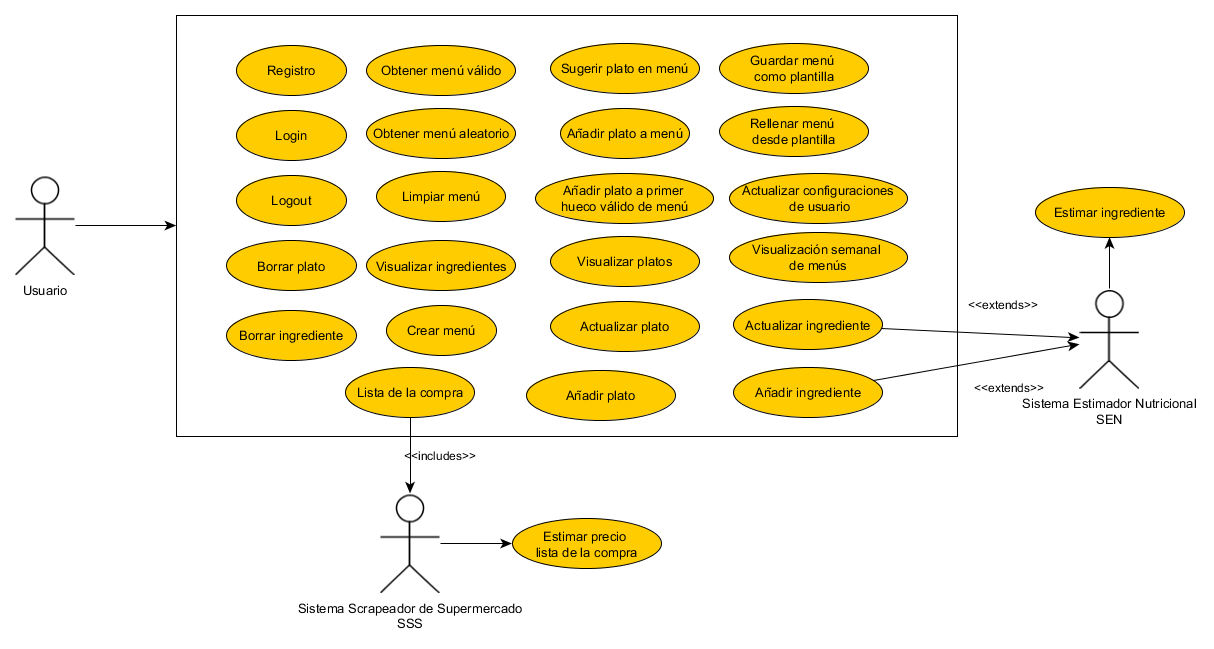
\includegraphics[width=15cm]{Imagenes/CasosUso.png}
		\caption{Casos de uso}\label{Casos de uso}
	\end{figure}
	\chapter{Diseño de la aplicación}
	Realizamos un diseño previo a la implementación para identificar los componentes necesarios para cumplimentación de los requisitos.	
	\section{Mockups}
	Para el diseño de la interfaz de usuario se han elaborado diferentes Mockups que sirvan para ilustrar los diferentes formularios del sistema y sus funcionalidades
	\subsection{Diseño inicial}
	Al empezar el diseño del proyecto y hacer un análisis de sus funcionalidades principales, se realizó este diseño inicial en el que de un vistazo se vieran los elementos básicos del sistema. A partir de él se elaboraron diseños más concretos sobre los diferentes formularios recogidos en él.
	\begin{figure}[H]
		\centering
		\includegraphics[width=10cm]{Imagenes/InitialDesign.jpg}
		\caption{Initial Design}\label{Initial Design}
	\end{figure}	
	\subsection{Planificacion Semanal de Menu}	
	
	La funcionalidad principal del sistema consistirá en un formulario en el que se pueda planificar el menú semanal, sus platos, los días y comidas a los que están asignados, los stats nutricionales de la combinación de esos platos y qué tal cumplen esos stats con los límites autoimpuestos por el usuario.
	
	\begin{figure}[H]
		\centering
		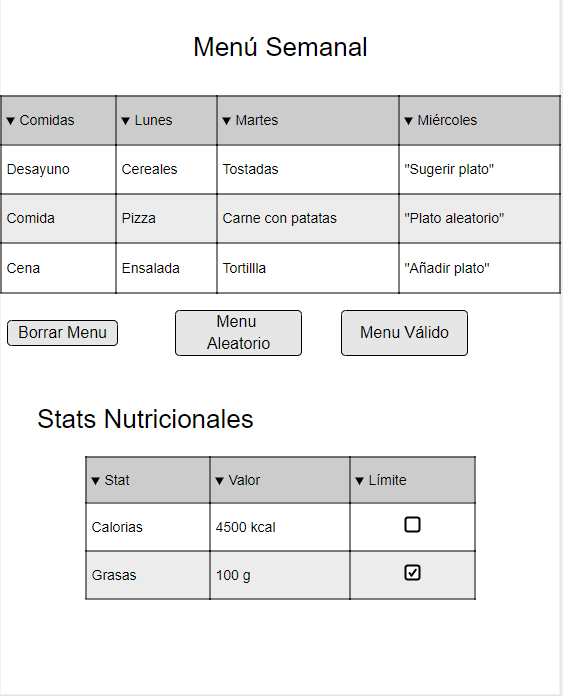
\includegraphics[width=10cm]{Imagenes/MockupMenuSemanal.png}
		\caption{Mockup Menu Semanal}\label{Mockup Menu Semanal}
	\end{figure}

	\subsection{Añadir ingrediente}	

	En el diseño de los formularios de inserción de las entidades del sistema intentamos optar por la mayor simplificidad posible.\\
	El formulario de añadir ingrediente permitirá indicar el nombre del nuevo ingrediente y sus stats nutricionales. 
	Se permitirá, a partir del nombre del ingrediente, estimar los stats de alguna forma automática.

	\begin{figure}[H]
		\centering
		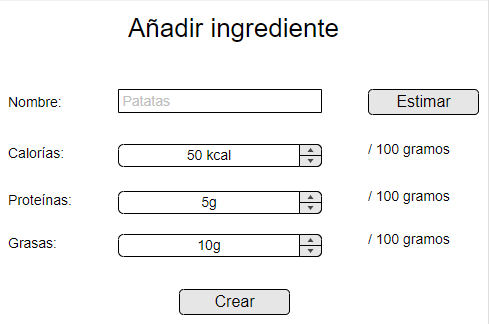
\includegraphics[width=10cm]{Imagenes/MockupAddIngredient.png}
		\caption{Anadir Ingrediente}\label{Anadir Ingrediente}
	\end{figure}

	\subsection{Añadir plato}	
	
	En el formulario de añadir plato se permitirá añadir los ingredientes que lo componen y, para cada uno, sus cantidades dentro del plato. \\
	A mayores se permitirá indicar la receta necesaria para la elaboración del plato y su nombre.
	
	\begin{figure}[H]
		\centering
		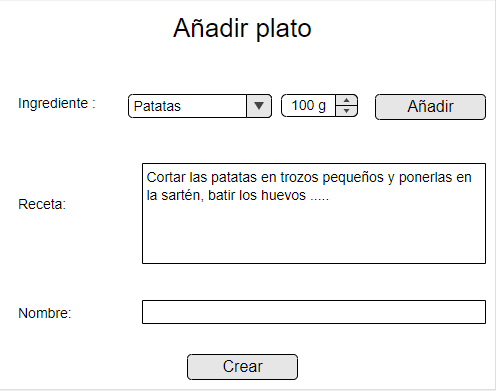
\includegraphics[width=10cm]{Imagenes/MockupAddDish.png}
		\caption{Anadir Plato}\label{Anadir Plato}
	\end{figure}

	\section{Diseño componentes del API}
	
	Para el diseño del modelo del negocio necesario, realizamos una primera fase en la que identificamos las entidades que componen los datos de nuestro sistema. Se obtienen las siguientes entidades de ese análisis:
	
	\subsection{Menú}
	
	Para la gestión de los menús, se ve una aplicación clara del Patrón Composición de forma que un Menú podrá estar compuesto por platos completos o bien por ingredientes. 
	El patrón Composición sirve para construir objetos complejos a partir de otros más simples y similares entre sí, gracias a la composición recursiva y a una estructura en forma de árbol.
	Esto simplifica el tratamiento de los objetos creados, ya que al poseer todos ellos una interfaz común, se tratan todos de la misma manera. Dependiendo de la implementación, pueden aplicarse procedimientos al total o una de las partes de la estructura compuesta como si de un nodo final se tratara, aunque dicha parte esté compuesta a su vez de muchas otras \cite{Patrones}
	En nuestra aplicación del patrón Composición, Ingredient representa el nodo hoja y Plato es una composición de Ingredientes. Técnicamente podríamos añadir el Menú como una composición de Platos pero preferimos no hacerlo ya que permitiría tratar un Menú como un Plato y queremos que en el sistema tengan funcionamientos totalmente diferentes.
	
	\begin{figure}[H]
		\centering
		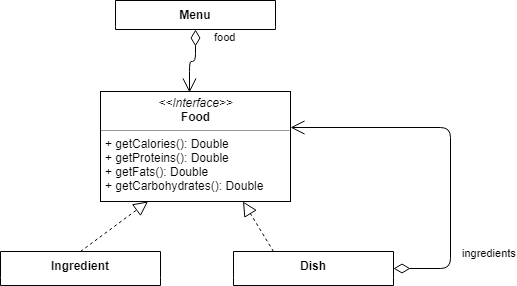
\includegraphics[width=10cm]{Imagenes/Menu.png}
		\caption{Menu}\label{Menu}
	\end{figure}

	\subsection{Servicios externos}
	
	Durante el funcionamiento del sistema se utilizan varios servicios externos para mejorar la experiencia del usuario y aportarle valor sin necesidad de cargar con esa lógica en nuestro sistema.
	
	Para la utilización de estos servicios externos utilizamos dos patrones de diseño adecuados para aislar la lógica de esos servicios concreto y no acoplarla a nuestro sistema: Patrón estrategia para mantener varios posibles servicios externos que solucionaran la misma necesidad de nuestro sistema y patrón adaptador para transformar una interfaz en otra de tal modo que las clases de nuestro sistema utilicen el adaptador en lugar de la interfaz concreta del servicio externo.
	
	Los tres casos principales de servicios externos que invoca el sistema son los siguientes:
	
	\begin{itemize}
		\item Edamam Nutrition Analysis API -\> Para evitar que el usuario deba registrar los stats nutricionales de cada uno de los ingredientes que ingresa en el sistema, se incorporan llamadas a esta API externa de estimación de calorías, proteínas y grasas a partir del nombre de ingrediente indicado por el user
		\begin{figure}[H]
			\centering
			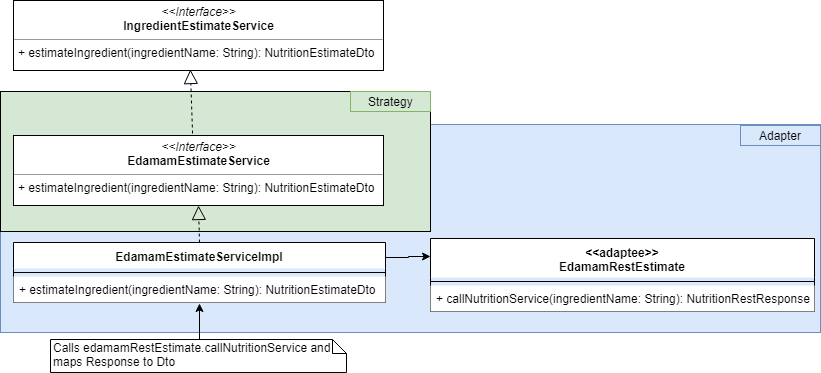
\includegraphics[width=15cm]{Imagenes/IngredientEstimateDesign.png}
			\caption{Ingredient Estimate}\label{Ingredient Estimate}
		\end{figure}
		\item Mercadona Price Estimation -\> Para estimar el precio de una posible lista de la compra del usuario, hemos utilizado un scrappeador que accede a la página web de Mercadona y descarga todo el catálogo con los siguientes datos: nombre del artículo y precio. A través de esta información, podemos, para una lista de la compra generada por el usuario, obtener una estimación del precio sumado de la compra de esos ingredientes en mercadona.
		\begin{figure}[H]
			\centering
			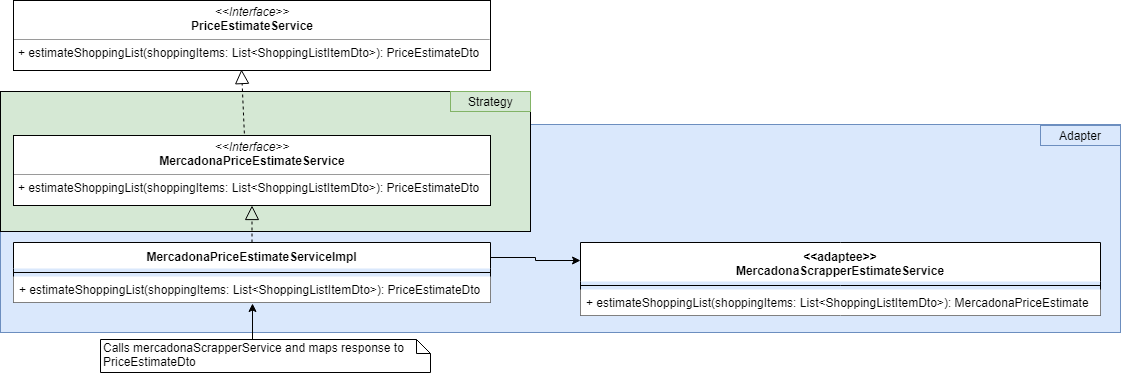
\includegraphics[width=15cm]{Imagenes/MercadonaPriceEstimate.png}
			\caption{Mercadona Price Estimate}\label{Mercadona Price Estimate}
		\end{figure}
		\item Weka Machine Learning Algorithm -\> Para la sugerencia de platos personalizada para cada usuario, utilizamos Weka, plataforma software de aprendizaje automático, para "predecir" el plato más conveniente para el usuario en el hueco del menú solicitado en función de los platos registrados por el usuario hasta el momento.
		\begin{figure}[H]
			\centering
			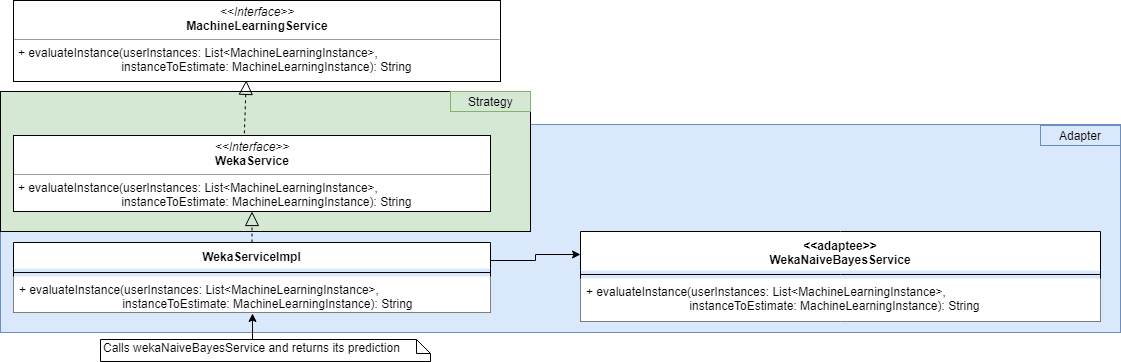
\includegraphics[width=15cm]{Imagenes/WekaService.png}
			\caption{Weka Service}\label{Weka Service}
		\end{figure}
	\end{itemize}

	\subsection{Modelo de Datos}
	A continuación se describirán todas las entidades principales de la aplicación.
	\begin{itemize}
		\item Descripción de entidades
		\begin{itemize}
			\item User \\Entidad representante de las personas que accederán a la misma. Es la entidad propietaria del resto de forma que puede tener Ingredientes, Platos, Menus ... asignados. Puede configurar gran parte de su funcionalidad en la aplicación mediante configuraciones de usuario.
			\item UserConfiguration \\ Cada una de las configuraciones de usuario que le permiten personalizar el funcionamiento del sistema para él en concreto como pueden ser : la cantidad de calorías por semana que se auto permite, las comidas al día que realiza y sus nombre ...
			\item Meal \\ Cada una de las comidas que se configura el usuario que le aparecen en sus calendarios y que puede permitir o restringir de sus platos. Tienen una hora asignada cada una de ellas para poder ordenarlas en la visualización de los calendarios.
			\item Ingredient \\ Cada uno de los ingredientes registrados por el usuario para su combinación en platos. Registran su nombre y sus stats nutricionales : calorías, proteinas, grasas y carbohidratos. Pueden pertenecer a una categoría alimenticia
			\item FoodCategory \\ Cada una de las categorías alimenticias a las que pueden pertenecer los ingredientes del usuario. Pueden ser prohibidas por el usuario para recordarse de que debe tener cuidado con esos ingredientes concretos.
			\item Dish \\ Cada uno de los platos que registra el usuario juntando de uno a varios ingredientes con una cantidad concreta y permitiendo especificar una receta de elaboración. Tienen stats nutricionales calculados como la suma de los stats de sus ingredientes en relación a su cantidad en el plato.
			\item Menu \\ Cada uno de los menú semanales que planifica el usuario del sistema. Están formados por un conjunto de platos asignados a una fecha concreta. Tienen stats nutricionales calculados como la suma de los stats de sus platos. Permiten obtener los elementos de su lista de la compra correspondiente como los ingredientes necesarios para todos sus platos con las unidades y la cantidad necesaria de cada uno.
		\end{itemize}
		\item Descripción de relaciones
		\begin{itemize}
			\item Relación Dish - Meal: Dispone de una relación N:M ya que un plato puede estar permitido en varias comidas del usuario y una comida tendrá varios platos permitidos.
			\item Relación Dish - Ingredient: Dispone de una relación N:M ya que un plato puede tener varios ingredientes y un mismo ingrediente puede aparecer en varios platos. Como atributo de la relación tenemos la cantidad que tendrá el ingredient en el plato concreto.
			\item Relación Dish - User: Dispone de una relación N:M ya que un plato puede aparecer en varios usuarios y un usuario puede tener varios platos.
			\item Relación Dish - Menu: Dispone de una relación N:M ya que un plato puede aparecer en varios menús y un menú tendrá por naturaleza varios platos. Como atributo de la relación tenemos la fecha concreta en la que el plato está registrado en el menú.
			\item Relación Ingredient - FoodCategory: Dispone de una relación 1:N ya que un ingrediente solo pertenecerá a una categoría pero una categoría tendrá varios ingredientes.
			\item Relación Ingredient - User: Dispone de una relación N:M ya que un ingrediente puede pertenecer a varios usuarios y un usuario puede tener varios ingredientes registrados.
			\item Relación User - Meal: Dispone de una relación 1:N ya que un usuario puede tener varias comidas registradas pero cada comida solo estará asignada a un usuario concreto.
			\item Relación User - UserConfiguration: Dispone de una relación 1:N ya que un usuario puede tener varias configuraciones pero cada configuración pertenecerá a un único usuario.
			\item Relación User - Menu: Dispone de una relación 1:N ya que un usuario puede tener varios menús registrados pero cada menú pertenecerá a un único usuario.
			\item Relación User - MenuTemplate: Dispone de una relación 1:N ya que un usuario puede tener varias plantillas de menú pero cada plantilla tendrá un único usuario.
			\item Relación Menu - MenuTemplate: Dispone de una relación 1:N ya que un menú puede generar varias plantillas pero cada plantilla pertenece a un único menú.
		\end{itemize}
	\end{itemize}	
	\subsubsection{Diagrama de Entidad Relación}
	A continuación, mostramos el diagrama entidad relación de base de datos empleado para la definición de las tablas, sus atributos y sus relaciones.
	\begin{figure}[H]
		\centering
		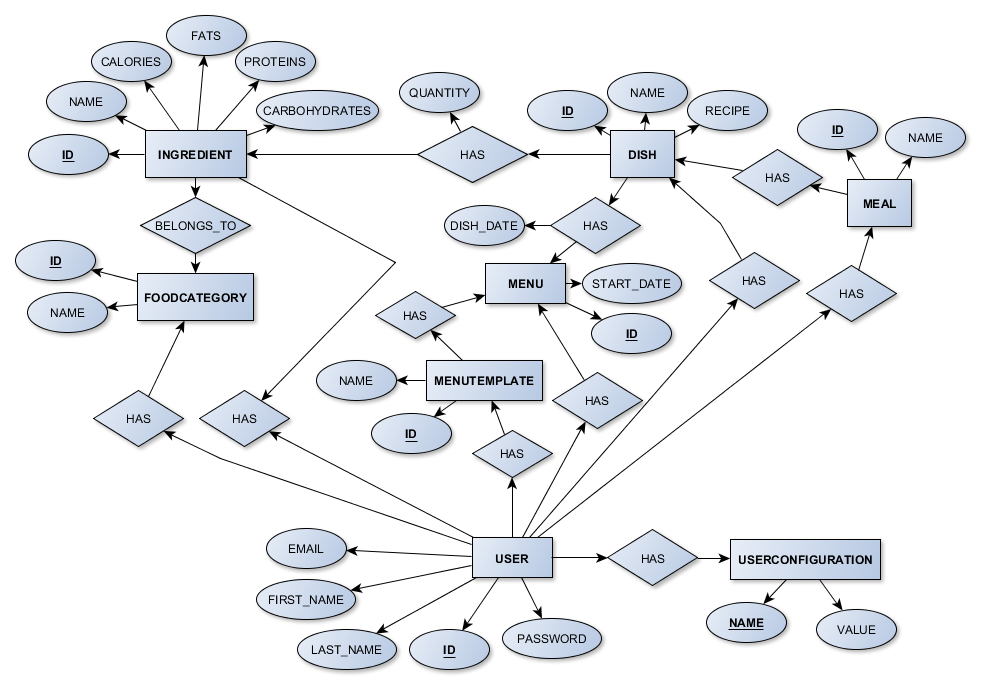
\includegraphics[width=15cm]{Imagenes/EntidadRelacion.png}
		\caption{Entidad relacion}\label{Entidad relacion}
	\end{figure}
	
	\section{Arquitectura general}
	
	La arquitectura del sistema es Cliente - Servidor para ello se subdivide en dos subsistemas correspondientes : efw-front (Cliente) y efw-back (Servidor).
	
	La arquitectura cliente-servidor es un modelo de diseño de software en el que las tareas se reparten entre los proveedores de recursos o servicios, llamados servidores, y los demandantes, llamados clientes. Un cliente realiza peticiones a otro programa, el servidor, quien le da respuesta. Esta idea también se puede aplicar a programas que se ejecutan sobre una sola computadora, aunque es más ventajosa en un sistema operativo multiusuario distribuido a través de una red de computadoras. \cite{Software Architecture}
	
	Las principales ventajas de esta arquitectura son las siguientes : 
	\begin{itemize}
		\item \textbf{Centralización del control:} los accesos, recursos y la integridad de los datos son controlados por el servidor de forma que un programa cliente defectuoso o no autorizado no pueda dañar el sistema. Esta centralización también facilita la tarea de poner al día datos u otros recursos
		\item \textbf{Escalabilidad:} se puede aumentar la capacidad de clientes y servidores por separado. Cualquier elemento puede ser aumentado (o mejorado) en cualquier momento, o se pueden añadir nuevos nodos a la red (clientes y/o servidores).
		\item \textbf{Fácil mantenimiento:} al estar distribuidas las funciones y responsabilidades entre varios ordenadores independientes, es posible reemplazar, reparar, actualizar, o incluso trasladar un servidor, mientras que sus clientes no se verán afectados por ese cambio (o se afectarán mínimamente).
		\item \textbf{Seguridad:} En las redes Cliente - Servidor los demás clientes no tienen acceso a las IP's por lo que se dificulta el rastreo y/o hackeo de los usuarios
	\end{itemize}
	
	La aplicación habitual de esta arquitectura acostumbra a delegar toda la carga de trabajo y de cálculos en el lado del servidor lo que, en sistemas de gran cantidad de usuarios simultáneos suele requerir hardware de grandes capacidades para este servidor(es) y una política de escalado vertical u horizontal para los picos de usuarios (En casos de ecommerce esto acostumbra ocurrir en periodos de rebajas, el sistema que se ha desarrollado no plantea estos puntos pero sigue presentado la necesidad de escalado en caso de gran popularidad y gran cantidad de usuarios simultáneos)
	
	Con la utilización del framework cliente Angular JS, se cambia el enfoque habitual para delegar parte de la carga en la máquina del usuario que accede. Esto tiene particular utilidad en la época actual en la que el hardware de los usuarios base es cada vez de mejores capacidades lo cual nos permite liberar al servidor de responsabilidad en favor de las máquinas del usuario. 
	
	A mayores, en esta arquitectura se ha aplicado el patrón MVC siendo el Modelo y la Vista dos artefactos totalmente diferentes que les permite ser independientes como se ve en la figura:
	
	\begin{figure}[H]
		\centering
		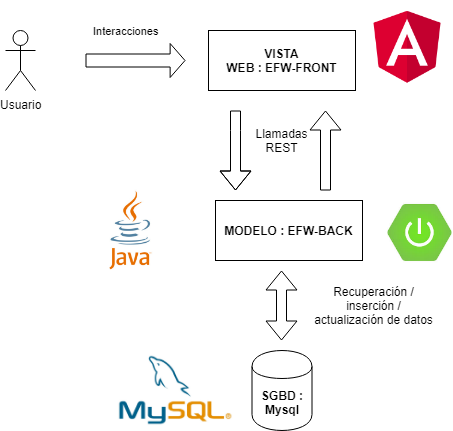
\includegraphics[width=10cm]{Imagenes/Arquitectura.png}
		\caption{Arquitectura global}\label{Arquitectura global}
	\end{figure}
	
	\section{Subsistema Backend efw-back}
	
	El backend del sistema está desarrollado como una serie de APIs REST totalmente aisladas del frontal de forma que sean independientes del mismo y puedan utilizarse por cualquier otro posible frontal que se requiera en el futuro (Aplicaciones nativas móviles, por ejemplo).
	
	\subsection{Arquitectura}		
	
	La arquitectura del backend se basa en la programación por capas, un modelo de desarrollo software en el que el objetivo primordial es la separación (desacoplamiento) de las partes que componen el sistema: lógica de negocios y capa de datos. De esta forma, por ejemplo, es sencillo y mantenible crear diferentes interfaces sobre un mismo sistema sin requerirse cambio alguno en la capa de datos o lógica.
	
	La ventaja principal de este estilo es que el desarrollo se puede llevar a cabo en varios niveles y, en caso de que sobrevenga algún cambio, solo afectará al nivel requerido sin tener que revisar entre el código fuente de otros módulos, dado que se habrá reducido el acoplamiento hasta una interfaz de paso de mensajes. \cite{Domain Driven Design}\\
	Además, permite distribuir el trabajo de creación de una aplicación por niveles; de este modo, cada grupo de trabajo está totalmente abstraído del resto de niveles, de forma que basta con conocer la API que existe entre niveles. Tenemos tres capas principales: La capa de acceso a datos y la capa de negocio, ambas representadas en el backend y se utilizan para acceder a la base de datos y ejecutar las lógicas de negocio del sistema para la transformación de los datos, respectivamente. Por último, tenemos la capa de presentación o de interacción con el usuario que está compuesta por efw-front y todos los componentes de Angular JS.
	Las APIs REST que provee el backend actúan como fachadas que nos permiten aislar esta capa de presentación de la capa de negocio marcando un "contrato" que la capa presentación debe cumplir para solicitar los datos necesarios para su visualización de la capa de negocio.\\
	
	Esta arquitectura se compone de cuatro elementos principales :
	
	\begin{itemize}
		\item Controladores REST que reciben cada una de las peticiones que realizará el frontal y se encargarán de validar que los parámetros de entradas de cada una de ellas se encuentran en el formato correcto con los datos necesarios y, en caso de no estarlo, pararán la petición devolverán un código y mensaje de error identificativos.
		\item Servicios, los principales contenedores de la lógica de negocio. Son invocados por los controladores y ellos a su vez invocan a los diferentes repositorios de acceso a datos para obtener la información necesaria para cada petición concreta. Preparan esta información en el formato necesario de la respuesta en caso de una petición de consulta o bien utilizarán los datos recibidos para hacer las actualizaciones correspondientes a una petición de actualización / modificación / borrado / inserciones.
		\item Repositorios, los encargados de las ejecuciones de las consultas / actualizaciones / borrados / inserciones sobre las propias bases de datos siguiendo las entidades configuradas.
		\item Entidades de base de datos de hibernate, cada una correspondiente a una tabla. Definen las columnas de su tabla correspondiente así como sus relaciones entre ellas.
	\end{itemize} 

	\begin{figure}[H]
		\centering
		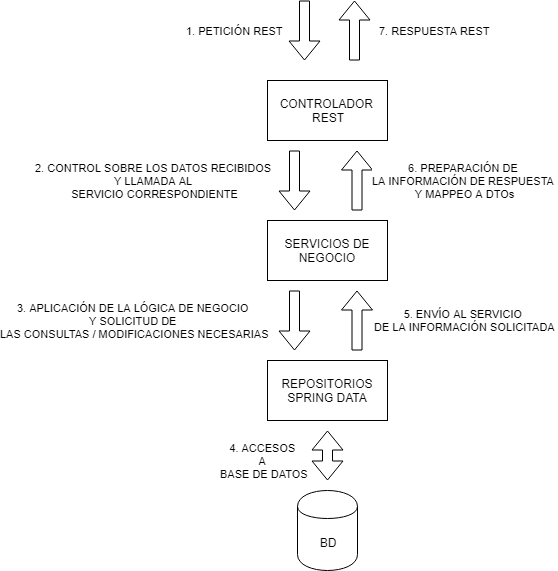
\includegraphics[width=12cm]{Imagenes/ArquitecturaBack.png}
		\caption{Arquitectura backend}\label{Arquitectura backend}
	\end{figure}
	
	\subsection{Modelo del dominio}    
	\subsubsection{Diagrama de Entidades}
	En la figura se muestra el diagrama de entidades de la aplicación.
	\begin{figure}[H]
		\centering
		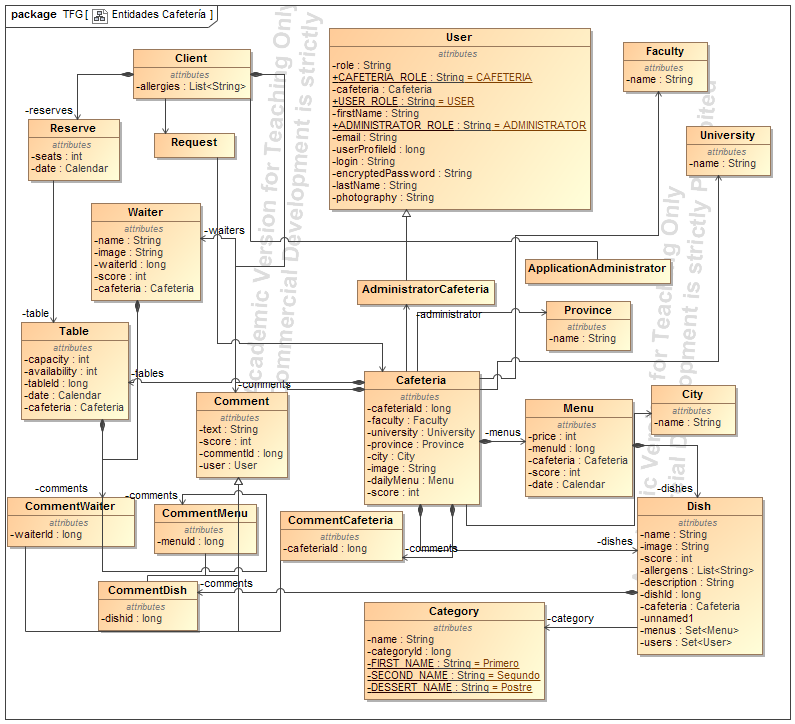
\includegraphics[width=15cm]{Imagenes/DiagramaClases.png}
		\caption{Diagrama de clases}\label{Diagrama de clases}
	\end{figure}	
	
	\subsection{Capa de Acceso a Datos}
	
	Empleamos repositorios implementados mediante Spring Data con lo que las consultas se infieren del nombre de los métodos a través de los atributos de la entidad de Hibernate utilizada en el repositorio concreto.
	
	Todos estos repositorios presentan métodos básicos de CRUD sobre su entidad correspondiente : 
	\begin{itemize}
		\item void delete(Entity e) -\> Elimina la entidad pasada como parámetro.
		\item List\<Entity\> findAll() -\> Obtiene todas las filas de esa entidad de base de datos sin ningún filtro aplicado.
		\item Entity findOne(int id) -\> Obtiene una fila concreta de la entidad correspondiente con el id único pasado como parámetro.
		\item Entity save(Entity e) -\> Inserta la entidad pasada como parámetro, o bien la actualiza en caso de ya existir previamente, con los datos guardados en el objeto del parámetro.
	\end{itemize}
	
	La aplicación presenta los siguientes repositorios:
	
	\begin{itemize}
		\item UserRepository: Además de las operaciones básicas de todos los repositorios dispone de un método de búsqueda de usuarios por email para el proceso de login de un usuario concreto a través de su email y contraseña.
		\item UserConfigurationRepository: Además de las operaciones básicas, dispone de un método de búsqueda de configuraciones de usuario por nombre de la configuración y el id del usuario al que se le quieren consultar las configuraciones.
		\item MenuTemplateRepository: Además de las operaciones básicas, dispone de un método de búsqueda de plantillas de menús para un usuario concreto.
		\item MenuRepository: Además de las operaciones básicas, dispone de un método de búsqueda de un menú a través de su id de usuario y de su fecha inicial.
		\item MenuDisRelRepository: Utilizado para dos operaciones de borrado concretas: Borrado por id de menú utilizado en la funcionalidad de limpiado de menú y borrado por ids (id de menú, fecha e id de plato) para las funcionalidades de borrado de plato de menú y la funcionalidad de actualización de fecha de plato en menú.
		\item MealRepository: Además de las operaciones básicas, dispone de una búsqueda por id de usuario ordenada por hora de la comida.
		\item IngredientRepository: Dispone de tres consultas custom : búsqueda de ingredientes por usuario para su visualización, búsqueda por usuario y nombre para verificar la unicidad del nombre de ingredientes en la inserción, búsqueda de otros ingredientes del usuario con mismo nombre para verificar la unicidad de nombre en la actualización
		\item FoodCategoryRepository: Dispone de una consulta custom para encontrar categorías que cumplan una lista de ids concretos para visualizar las categorías que el usuario tiene configuradas como prohibidas.
		\item DishRepository: Dispone de tres consultas custom : búsqueda de platos por usuario para su visualización, búsqueda por usuario y nombre para verificar la unicidad del nombre de platos en la inserción, búsqueda de otros platos del usuario con mismo nombre para verificar la unicidad de nombre en la actualización
		\item CustomQueryRepository: Disponemos de un repositorio concreto utilizado para una consulta concreta necesaria para la funcionalidad de Machine Learning cuya complejidad es demasiado grande para poder realizarla de forma eficiente con Spring Data. Para un usuario, obtiene de todos sus menús los tres valores siguientes : Día de la semana - Nombre de comida - Plato asignado a ese hueco. 	
	\end{itemize}
	
	\subsection{Capa Servicios del Modelo}
	Como comentábamos en el principio del subsistema backend, tenemos una serie de servicios de negocio para dar soporte a cada una de las peticiones REST permitidas. 
	Para cada uno de ellos se define una interfaz en la que se indican todos los métodos del servicio y su firma. Tenemos por otro lado una clase que implementa esta interfaz y todos sus métodos.
	\begin{itemize}
		\item DishService : 
		\begin{itemize}
			\item create: Servicio utilizado para crear nuevos platos. Se le indica el usuario para el que se quiere registrar, el nombre del plato, la receta, sus ingredientes y cada una de sus cantidades así como las comidas en las que el plato debe estar permitido. Lo primero que se verifica es que el usuario no tenga ya un plato con este nombre en cuyo caso se devolvería un error indicándolo. En caso contrario, se registra el plato con los datos informados.
			\item delete: Servicio utilizado para eliminar platos existentes por id. Se consulta el plato correspondiente al id informado. En caso de no existir, se devuelve un error indicándolo. En caso contrario se elimina el plato a través del repositorio.
			\item findUserDishes: Servicio utilizado para obtener todos los platos de un usuario a través del id del usuario. Los platos obtenidos se transforman para ceñirse al formato de respuesta de la petición: id de plato, nombre, receta, ingredientes y sus cantidades, comidas permitidas y lista de stats nutricionales del plato calculados como la suma de los de sus ingredientes en relación a su cantidad en el plato.
			\item update: Servicio utilizado para actualizar un plato existente. Se comprueba que existe un plato con el id indicado, en caso de no ser así se devuelve un error informativo. En caso de existir, se comprueba que el nuevo nombre a establecer no esté siendo usado por otro plato del usuario. En caso de no cambiar el nombre o bien de estar libre el nuevo nombre se actualiza la información indicada en el plato.
		\end{itemize}
		\item IngredientService : 
		\begin{itemize}
			\item create: Servicio utilizado para crear nuevos ingredientes. Se le indica el usuario para el que se quiere registrar, el nombre del ingrediente y sus stats: calorías, proteinas, grasas y carbohidratos. Lo primero que se verifica es que el usuario no tenga ya un ingrediente con este nombre en cuyo caso se devolvería un error indicándolo. En caso contrario, se registra el ingrediente con los datos informados.
			\item delete: Servicio utilizado para eliminar ingredientes existentes por id. Se consulta el ingrediente correspondiente al id informado. En caso de no existir, se devuelve un error indicándolo. En caso contrario se elimina el ingrediente a través del repositorio.
			\item findUserIngredients: Servicio utilizado para obtener todos los ingredientes de un usuario a través del id del usuario. Los ingredientes obtenidos se transforman para ceñirse al formato de respuesta de la petición: id de ingrediente, nombre, categoria alimenticia(id y nombre) y lista de stats nutricionales del ingrediente.
			\item update: Servicio utilizado para actualizar un ingrediente existente. Se comprueba que existe un ingrediente con el id indicado, en caso de no ser así se devuelve un error informativo. En caso de existir, se comprueba que el nuevo nombre a establecer no esté siendo usado por otro plato del usuario. En caso de no cambiar el nombre o bien de estar libre el nuevo nombre se actualiza la información indicada en el ingrediente.
			\item getNutritionEstimate: Servicio de obtención de los stats nutricionales de un ingrediente a través de su nombre. Se delega en el servicio rest externo de estimación de stats nutricionales por ingrediente para estimarlos a través del nombre de ingrediente recibido como parámetro. Se transforman los stats recibidos con la cantidad de ingrediente recibida para transformarlos de forma que se muestren "/ 100 gramos".
			\item getFoodCategories: Servicio de obtención de todas las categorías alimenticias delegando la consulta en el repositorio de categorías alimenticias.
		\end{itemize}
		\item MachineLearningService : 
		\begin{itemize}
			\item evaluateInstance: Servicio utilizado para, a través de Weka, predecir el nombre del plato predicho para un Día de Semana y una Comida concreta. El servicio recibe la lista de todas las combinaciones registradas de {Día de semana, Comida, Nombre de plato} de ese usuario hasta el momento. Con estos datos se entrena la el clasificador para que pueda predecir la nueva instancia solicitada. Se devuelve la predicción en forma de nombre de plato.
		\end{itemize}
		\item MenuService :
		\begin{itemize}
			\item create: Servicio utilizado para crear nuevos menús. Se le indica el usuario para el que se quiere registrar y la fecha de inicio del menú a crear. La fecha recibida puede corresponderse con cualquier de la semana con lo que, a partir de ella, obtenemos el inicio de semana más cercano hacia atrás en el tiempo (En caso de recibirse un domingo 25 se obtiene el lunes 19 por ejemplo). Este lunes se establece en el menú a crear y se crea a través del repositorio de menús.
			\item clearMenu: Servicio utilizado para limpiar el menú de platos a través del id del menú. En caso de no encontrarse un menú con este id se devuelve un error indicativo. En caso de encontrarse, se borran todas las relaciones entre este menú y sus platos de forma que el menú queda vacío.
			\item findUserMenu: Servicio utilizado para obtener el menú de un usuario en una fecha dada. A través de la fecha recibida se obtiene el inicio de semana más cercano como se hace en la creación de menús.
			\item addDishToMenu: Servicio utilizado para añadir un plato a un menú. Se reciben el id del menú, el id del plato y la fecha en la que se quiere añadir. Se buscan el menú y el plato por los ids, en caso de no encotnrarlos, se devuelve un error significativo. En caso contrario se registra la nueva relación entre el menú y el plato en la fecha correspondiente.
			\item addDishToFirstValidSpotOnMenu: Servicio uilizado para añadir un plato al hueco válido más temprano posible de un menú. Se reciben el id del usuario al que pertenece el menú así como el id del plato que se quiere añadir. Primero, se obtiene el menú actual del usuario a través del id de usuario y el inicio de semana correspondiente al día actual. A continuación se busca el hueco disponible más cercano para el menú y el plato, la fecha más cercana con una comida permitida por el plato.
			\item updateDishDateOnMenu: Servicio utilizado para actualizar la fecha de un plato en un menú. Se reciben el id del menú, el id del plato, la fecha actual en el menú y la fecha nueva que se desea. A través de estos datos se obtiene la relación entre el plato y el menú, se elimina y se monta la nueva relación con la nueva fecha.
			\item removeDishFromMenu: Servicio utilizado para eliminar la relación de un plato y un menú en una fecha concreta. Se reciben el id del menú, el id del plato y la fecha de la relación que se quiere eliminar. Se obtiene la relación a través de estos datos y se elimina.
			\item getShoppingList: Servicio utilizado para obtener la lista de la compra de un menú. Se recibe el id del menú. A través del menú, se obtienen los ingredientes de cada uno de sus platos, se agrupan y se obtiene tanto el número de veces que aparece cada ingrediente como la cantidad total en gramos de los ingredientes. En este método se delega en el servicio de estimación de precio de mercadona que utiliza los datos scrappeados del catálogo de mercadona para sacar una estimación del precio total de la lista de la compra generada.
			\item randomGenerateMenu: Servicio utilizado para rellenar un menú con los platos del usuario aleatoriamente. Se recibe el id del menú, en caso de no estar ya vacío, se limpia de platos el menú y a continuación se rellena aleatoriamente con los platos del usuario. Se itera por los días del menú y en cada comida del día se selecciona aleatoriamente un plato de entre los platos del usuario que tienen permitida esa comida.
			\item generateValidMenu: Servicio utilizado para rellenar un menú de forma que no se incumplan los límites de stats del usuario. Se recibe el id del menú, en caso de no estar ya vacío, se limpia de platos el menú y a continuación se rellena válidamente con los platos del usuario. Se itera por los días del menú y en cada comida del día se selecciona un plato válido para ese hueco : que tenga esa comida permitida y cuyos stats más los que tenemos por el momento en el menú no incumplan algunos de los límites del usuario. En caso de no poder seleccionar ningún plato, se para la generación del menú y se deja rellenado hasta lo máximo que podemos.
			\item fillMenuFromTemplate: Servicio utilizado para rellenar un menú a través de una plantilla. Se reciben el id del menú a rellenar y el id de la plantilla a aplicar. Se consulta el menú a rellenar, en caso de no estar ya vacío, se vacía de platos y se rellena con los platos registrados en la plantilla en los huecos correspondientes en el nuevo menú.
			\item machineLearningSuggestDish: Servicio utilizado para predecir el Plato correcto para un hueco de menú en función de los gustos del usuario. Se reciben el id del menú y la fecha en la que se quiere obtener el plato sugerido. Se delega en el repositorio de queries custom para obtener para el usuario todas las tuplas {Día de semana, Comida, Nombre de plato} de los menús registrados en el sistema del usuario. Se delega en el servicio de machine learning para obtener el plato sugerido en función de estos datos y, en caso de obtenerse un plato, se agrega al menú en el hueco indicado.
		\end{itemize}
		\item MenuTemplateService :
		\begin{itemize}
			\item saveMenuAsTemplate: Servicio utilizado para generar una plantilla a través de un menú. Se reciben el id del menu que se quiere utilizar para generar la plantilla, el nombre que se le quiere asignar y el menú en el que inspirar la plantilla. Se obtiene el menu y el usuario a traves de sus ids y se genera la nueva plantilla a través de los platos del menú obtenido y se registra en el usuario.
		\end{itemize}
		\item MercadonaPriceEstimateService : 
		\begin{itemize}
			\item estimateShoppingList: Servicio utilizado para estimar el precio de una lista de la compra en función de los precios de mercadona. Se reciben los elementos de la lista de la compra y sus unidades. Se procesa el excel obtenido a través de los scrapeos de la página web de mercadona, se buscan los elementos de la lista de la compra en este excel y se accede a sus precios.
		\end{itemize}
		\item UserConfigurationService :
		\begin{itemize}
			\item findUserConfigurationByNameOrDefault: Servicio utilizado para obtener el valor de una configuración de usuario por nombre e id de usuario. Se reciben el id de usuario, el nombre de la configuración, la clase a la que se debe castear el valor de la configuración y un valor por defecto que se devolverá en caso de no encontrarse la configuración consultada.
			\item findUserConfigurationListByNameOrDefault: Servicio utilizado para obtener el valor de una configuración de usuario en forma de lista. Se parseará el valor de la configuración con la clase indicada y se dividirá el valor de la configuración en elementos de la lista a devolver separados en el valor por ","
		\end{itemize}
		\item UserDataLoadService : Servicio utilizado para obtener los datos por defecto que se cargarán en un usuario al registrarlo por primera vez en el sistema.
		\begin{itemize}
			\item getDefaultMeals: Método utilizado para obtener las comidas por defecto que se cargan en nuevos usuarios. Tienen los valores : Desayuno, Comida y Cena.
		\end{itemize}
		\item UserService: 
		\begin{itemize}
			\item create: Método utilizado para registrar un nuevo usuario en el sistema. Recibe un nombre, un apellido, un email y una constraseña que se registrarán en el nuevo usuario. Se delega en el servicio de userDataLoad para cargar los datos por defecto de nuevos usuarios.
			\item updateUserConfigurations: Método utilizado para cambiar los valores de las configuraciones de usuario indicadas. Se reciben el id de usuario cuyas configuraciones cambian y los nuevos valores a cargar en ellas.
			\item findConfigurations: Método utilizado para obtener los valores de las configuraciones de usuario de un usuario concreto. Se recibe el id del usuario a consultar, se consultan sus configuraciones y se formatean para poder devolverlas con nombres y tipos concretos.
			\item login: Método utilizado para iniciar sesión con un usuario concreto. Se reciben un email y una contraseña que intentan iniciar sesión en el sistema. Se comprueba si se corresponden con los de algún usuario y en caso de corresponderse se devuelve login correcto. En otro caso se devuelve el error concreto.
		\end{itemize}
	\end{itemize}
	
	\section{Subsistema Frontend efw-front}
	
	El frontal Web desarrollado utiliza Angular JS y su arquitectura se centra en módulos y su subdivisión en componentes.
	
	Como hemos comentado anteriormente, en el diseño del sistema se ha seguido el patrón Modelo Vista Controlador, patrón de arquitectura de software, que separa los datos y la lógica de negocio de una aplicación de su representación y el módulo encargado de gestionar los eventos y las comunicaciones. Para ello MVC propone la construcción de tres componentes distintos que son el modelo, la vista y el controlador, es decir, por un lado define componentes para la representación de la información, y por otro lado para la interacción del usuario. Este patrón de arquitectura de software se basa en las ideas de reutilización de código y la separación de conceptos, características que buscan facilitar la tarea de desarrollo de aplicaciones y su posterior mantenimiento. \cite{Patrones}
	
	Dentro de este patrón, efw-front representa la Vista, pero debido a la utilización del patrón se permite sin problema la incorporación en el futuro de nuevas Vistas como podrían ser aplicaciones nativas Android o iOS, o bien, una aplicación de escritorio.
	
	Dentro del funcionamiento que utilizamos de Angular se emplea el Patrón Observador, patrón de diseño de software que define una dependencia del tipo uno a muchos entre objetos, de manera que cuando uno de los objetos cambia su estado, notifica este cambio a todos los dependientes. Se trata de un patrón de comportamiento, por lo que está relacionado con algoritmos de funcionamiento y asignación de responsabilidades a clases y objetos. Este patrón es la base de la comunicación entre el Modelo y la Vista y se aplica en el sistema en las llamadas REST a efw-back. Cada vez que realizamos una petición al backend observamos en segundo plano y, en cuanto obtenemos una respuesta, modificamos la visualización en función de los nuevos datos obtenidos. También se emplea en la comunicación de algunos de los componentes de Angular de la forma que por ejemplo el componente de visualización de estadísticas nutricionales de un menú se subscribe a posibles cambios en las estadísticas nutricionales de ese menú (por la añadición de un nuevo plato, o la eliminación de alguno de los ya registrados)
	
	Cada componente presenta los siguientes elementos : 
	\begin{itemize}
		\item Hoja de estilos CSS -\> Los estilos necesarios para el html que forma el componente
		\item Plantilla HTML -\> Los elementos que conforman la visualización del componente
		\item Controlador Typescript -\> El controlador de los elementos definidos en la plantilla html. Contiene el servicio encargado de los datos. El propio controlador se centra en la gestión de las visualizaciones del componente.
		\item Servicio Typescript -\> Contenedor de los cálculos de datos realizados en el frontal. Son también los responsables de las llamadas rest a los servicios expuestos por el backend.
	\end{itemize}

	\begin{figure}[H]
		\centering
		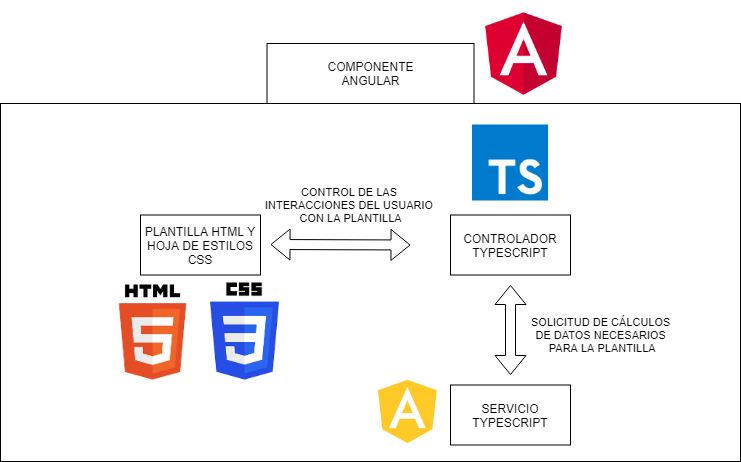
\includegraphics[width=12cm]{Imagenes/DiagramaComponente.png}
		\caption{Diagrama Componente Angular}\label{Diagrama Componente Angular}
	\end{figure}

	\subsection{Módulos empleados}
	
	Se definen los siguientes módulos agrupados por dominio : 
	
	\subsubsection{Módulo Calendar}
	El encargado de la gestión de calendarios semanales genéricos que luego aplicaremos para nuestra lógica del sistema. Contiene los siguientes componentes : 
	\begin{itemize}
		\item calendar-header : Correspondiente con la cabecera del calendario en la que se muestra la paginación de calendarios semanales.
		\item calendar-week-view : Componente contenedor del calendario con cada uno de los días y sus comidas.
		\item calendar-week-view-add-dish : Pop up utilizado para seleccionar un plato para añadir al calendario.
		\item calendar-week-view-event : Componente con cada uno de los platos de los calendarios.
		\item calendar-week-view-header : Componente de mostrado de la semana actual del calendario seleccionado.
		\item calendar-week-view-hour-segment : Componente correspondiente con cada uno de los huecos del calendario : Combinación de día y comida concreta de ese día.
		\item calendar-week-view-shopping-list : Pop up en el que se visualiza la lista de la compra correspondiente a un menú concreto.
	\end{itemize}
	\subsubsection{Módulo Dish}
	El encargado de la gestión de los formularios correspondientes con la entidad plato, tanto creación como listado y actualización. Contiene los siguientes componentes : 
	\begin{itemize}
		\item add-dish : Componente de creación de platos. Permite seleccionar los datos necesarios para la creación de un nuevo plato del usuario y contiene el componente Nutrition.view-stats para visualizar los stats del plato antes de añadirlo.
		\item dishes : Componenete de visualización de platos de usuario. Se permiten ver los nombres de cada plato y sus stats así como actualizarlos, borrarlos y añadirlos de forma automática al primer hueco válido del menú actual
		\item update-dish : Componente de actualización de un plato. Se carga automáticamente con los datos del plato seleccionado y a partir de ahí funciona de forma igual que el formulario de añadir plato.		
	\end{itemize}
	\subsubsection{Módulo Ingredient}
	El encargado de la gestión de los formularios correspondientes con la entidad ingrediente, tanto creación como listado y actualización. Contiene los siguientes componentes : 
	\begin{itemize}
		\item add-ingredient : Componente de creación de ingredientes. Permite rellenar su nombre y sus stats nutricionales. Una vez rellenado el nombre, se puede estimar sus stats a través de un botón de estimación para facilitar la experiencia del usuario y evitarle trabajo extra.
		\item ingredient : Componenete de visualización de ingredientes de usuario. Se permiten ver los nombres de cada ingrediente, su categoría alimenticia, sus stats y un warning en caso de que su categoría esté marcada como prohibida para el usuario. Se permite también actualizar y borrar los ingredientes mostrados.
		\item update-ingredient : Formulario de actualización de ingrediente. Se carga automáticamente con los datos del ingrediente seleccionado y a partir de ahí funciona de forma igual que el formulario de añadir ingrediente.
	\end{itemize}
	\subsubsection{Módulo Menu}
	El encargado de la gestión de los menús semanales del usuario. Contiene los siguientes componentes : 
	\begin{itemize}
		\item menu-calendar : Componente principal de visualización del menú semanal. Contiene el componente Calendar.calendar-week-view y el componente Nutrition.view-stats-dashboard. Desde este componente se permite crear un nuevo menú cuando el sistema detecta que en la semana actual no existe un menú para el user, se permite obtener la lista de la compra del menú actual, limpiarlo de platos, llenarlo aleatoriamente, llenarlo de forma que no se incumplan los límites nutricionales del user, guardar el menú actual como plantilla, llenar el menú actual a través de una plantilla e imprimir el menú actual.
		\item menu-save-template : Pop up utilizado para permitir al user indicar un nombre a la plantilla antes de guardarla con los platos del menú actual.
		\item menu-select-template : Pop up utilizado para seleccionar la template que utilizará el usuario para llenar el menú actual.
	\end{itemize}
	\subsubsection{Módulo Nutrition}
	El encargado de la visualización de los stats nutricionales de las diferentes entidades del sistema. Contiene los siguientes componentes : 
	\begin{itemize}
		\item view-stats-dashboard : Componente encargado de la gestión de la visualización de los stats de un menú. Contiene el componente Nutrition.view-stats para su visualización. Permite al usuario seleccionar dos modos principales de visualización : SEMANAL, donde se muestran los stats de toda la semana sumados y DIARIA, donde se muestran los stats de un día seleccionado por el usuario.
		\item view-stats : Componente encargado de la visualización de unos stats nutricionales. Reaprovechado para tanto la visualización de los de un plato como los de un menú.
	\end{itemize}
	\subsubsection{Módulo User}
	El encargado de la gestión de los formularios de cada usuario. Contiene los siguientes componentes : 
	\begin{itemize}
		\item add-user : Componente encargado de dar de alta nuevos usuarios en el sistema, se debe indicar para ello un nombre, un apellido, un email y una contraseña.
		\item login : Componente encargado de iniciar sesión en el sistema a través del email y contraseña del usuario. También permite iniciar sesión en el sistema a través de su cuenta de Facebook si así lo desea.
		\item user-confs : Componente encargado de la visualización y de la actualización de las configuraciones de usuario. Se carga automáticamente con los valores actuales de esas configuraciones para ese usuario y le permite modificar esos valores.
	\end{itemize}
	
	\chapter{Implementación}
	\section{Software requerido}
	Como se ha especificado con anterioridad, para la implementación del sistema hemos decidido el uso del IDE Eclipse, Spring, Hibernate y Spring Data para el acceso a datos y el modelo, Angular JS y Typescript para la interfaz visual y MySQL como base de datos.
	\section{Proceso seguido}
	Durante la implementación del \textbf{backend} se ha buscado en todo momento la \textbf{eficiencia}, minimizando el número de \textbf{consultas} necesarias y el número de \textbf{bucles} utilizados para el procesamiento de la información requerida. Este es un factor importante debido a la necesidad de la escalabilidad detectada en nuestro sistema.\\
	En este segundo apartado cabe destacar que nos hemos aprovechado de las ventajas que ofrece Java 8 con sus \textbf{streams y lambdas} soportados para hacer toda posible iteración lo más eficiente posible y legible en el código resultante.\\
	Nuestras elecciones tecnológicas con Spring Data como gestor de consultas y Mapstruct como mapeador de entidades de hibernate a dtos enviados en la respuesta REST nos han permitido garantizar un buen nivel de agilidad en el desarrollo del backend ante cambios sobre operaciones ya existentes que requieran un nuevo campo de respuesta al solo necesitar declarar el nuevo campo en la entidad de hibernate y en el dto de respuesta haciendo Mapstruct el mapeo automático al utilizar el mismo nombre en los dos objetos.\\
	Durante la implementación del \textbf{frontend} se ha buscado que los componentes definidos sean lo más acotados, independientes y reutilizables posibles para poder minimizar la repetición de código y aumentar su legibilidad. Se ha intentado que cada componente delege todos sus cálculos y lógica necesarios en sus servicio asignado y deje al controlador typescript las funciones de visualización de sus elementos HTML lo que hace que cada fichero tenga una responsabilidad clara y minimiza su número de líneas para seguir mejorando la legibilidad.\\
	Nos hemos preocupado de definir los estilos comunes del sistema en el fichero CSS de nivel más raíz posible para evitar su repetición en cada una de las hojas de estilos de los componentes utilizados.
	\section{Generación de menú aleatortio}
	Dentro de la implementación del api rest queremos destacar el algoritmo de generación de menú aleatorio ya que lo vemos como un punto de interés en su implementación dentro de las diferentes operaciones rest que se aportan al frontal. \\Vamos a ver el proceso completo de la petición desde el punto en el que se inicia desde el frontal hasta que se ejecuta su lógica, se informa de que se ha generado correctamente y el frontal actualiza la vista.\\
	\subsection{Componente AngularJS: menu-calendar}
	Esta opción del sistema se permite desde la visión de calendario semanal en la botonera del menú
	\subsubsection{Plantilla HTML}
	Para permitir que el usuario solicite la funcionalidad al sistema le mostramos un botón HTML cuya acción de click será manejada por el controlador typescript del componente.
	\begin{lstlisting}
		// Plantilla HTML : menu-calendar.component.html
		<button (click)="randomMenu()"><b>Random menu</b></button>
	\end{lstlisting}
	\subsubsection{Controlador TypeScript: MenuCalendarComponent}
	Desde el controlador del componente llamamos al servicio que representa el API de menús y nos subscribimos a su respuesta. 
	En cuanto la recibimos, consultamos al API el menú de nuevo para ver su nueva configuración de platos, inicializamos la visión de platos con ella y enviamos al componente de visualización de stats nutricionales un aviso de que debe reflejar los cambios. Todo esto se realiza sin necesidad de recargar la página y a gran velocidad.
	\begin{lstlisting}
		// Controlador Typescript : menu-calendar.component.ts
		randomMenu() {
			this.menuService.randomGenerateMenu(this.menu.id, this.currentUser.id, null, null).subscribe(data => {
				this.initMenuAndEvents();
			});
		}
		this.menuService.getUserMenu(this.currentUser.id, this.viewDate).subscribe(data => {
			if (data.id === null) {
				this.menu = null;
			} else {
				this.menu = data;
				this.events = this.initCalendarEventsWithDishes();
				this.sendUpdateStatsEvent();
			}
		});
	\end{lstlisting}
	\subsubsection{Servicio TypeScript de llamada al API de menús: MenuService}
	Desde el servicio typescript hacemos la llamada al API con los parámetros especificados. Al tener queryParams opcionales (startDate y endDate) debemos revisar si se nos han especificado o no antes de incluirlos en la llamada.
	En caso de que se hubiera realizado la llamada desde webMobile o webTablet se habrían indicado los dos queryParams startDate y endDate para indicar al backend el rango de fechas para el que se quiere generar el menú aleatorio, al no haberse hecho, se genera para toda la semana.
	\begin{lstlisting}						
		// Menu Service TypeScript: menu-service.ts
		public randomGenerateMenu(menuId: number, userId: number, startDate: string, endDate: string) {
			let params = new HttpParams().set('userId', userId.toString());
			if (startDate) {
				params = params.set('startDate', startDate);
			}
			if (endDate) {
				params = params.set('endDate', endDate);
			}
			return this.http.post<Menu>(this.menuUrl + '/' + menuId + '/random', {}, { params: params });
		}
	\end{lstlisting}
	\subsection{Controlador REST: MenuController}
	Al recibir la llamada del frontal el controlador REST de Spring verifica que se ha hecho con los parámetros correcto y que se cumple con la especificación del API. En este caso reconoce el queryParam userId y el pathParam menuId.	
	Una vez validados los parámetros recibidos, llamamos al servicio de negocio, MenuServiceImpl y devolvemos el resultado.
	\begin{lstlisting}
	@CrossOrigin(origins = "*", maxAge = 3600)
	@RestController
	@RequestMapping({ "/menus" })
	public class MenuController {
		@Autowired
		private MenuService service;
		...
		@PostMapping(path = { "/{id}/random" })
		public ResponseDto randomGenerate(@PathVariable("id") int menuId, @RequestParam("userId") Integer userId,
			@RequestParam(value = "startDate", required = false) String startDate,
			@RequestParam(value = "endDate", required = false) String endDate) {
			return service.generateRandomMenu(menuId, userId, startDate, endDate);
		}
		...
	}
	\end{lstlisting}
	
	\subsection{Servicio de negocio: MenuServiceImpl}
	Dentro de MenuServiceImpl tenemos los siguientes métodos que se utilizan para obtener, a partir del id de menú, id de usuario y fechas de inicio y fin de generación del menú, un menú aleatorio entre las dos fechas.\\
	
	\begin{lstlisting}
	@Override
	@Transactional
	public ResponseDto generateRandomMenu(Integer menuId, Integer userId, String startDate, String endDate) {
		// First, we query the necessary info : The menu, user dishes and number of meals
		Menu menu = this.repository.findOne(menuId);	
		List<Dish> userDishes = this.dishRepository.findUserDishes(userId);
		Integer mealsInWeek = this.userService.findUserMeals(userId).size();
		
		...
		
		// We iterate over the correct date range
		while (startDate.compareTo(endDate) <= 0) {
			// We fill each day with random valid dishes
			fillDayWithRandomDishes(menu, userDishes, startDate, endDate);
			startDate = startDate.plusDays(1L);
		}	
		
		// We persist the changes on the menu
		menu = this.repository.save(menu);
		
		// We return a message indicating that the operation has been a success
		return new ResponseDto(ResponseDto.OK_CODE, "Menu random generated correctly");
	}
	
	private void fillDayWithRandomDishes(Menu menu, List<Dish> userDishes, LocalDateTime date, Integer mealsInWeek) {
		for (int i = 0; i < mealsInWeek; i++) {
			// Select a random valid dish
			Dish randomDish = selectRandomDishWithValidMeal(userDishes, date);
			if (randomDish != null) {
				// Add it to the menu
				MenuDisRel mdr = new MenuDisRel(new MenuDisRelId(menu, randomDish,
				date.format(DateTimeFormatter.ofPattern("yyyy-MM-dd HH:mm:ss.S"))));
				menu.getDishes().add(mdr);
			}
			date = date.plusHours(1L);
		}
	}
	
	// We'll try to select a dish whose meals are accord with the date
	// If we can't, we return null
	private Dish selectRandomDishWithValidMeal(List<Dish> userDishes, LocalDateTime date) {
		Dish validDish = null;
		String hourFormatted = date.format(DateTimeFormatter.ofPattern("HH"));
		// We filter the dishes by those with any available meal that matches the date
		List<Dish> validDishes = userDishes.stream().filter(dish -> dish.getMeals().stream()
		.map(meal -> meal.getId().getMeal()).anyMatch(m -> hourFormatted.equals(m.getHour())))
		.collect(Collectors.toList());
		if (!validDishes.isEmpty()) {
			validDish = randomSelectDish(validDishes);
		}
		return validDish;
	}
	
	private Dish randomSelectDish(List<Dish> userDishes) {
		Random random = new Random();
		Integer randomIndex = random.nextInt((userDishes.size() - 1)  + 1);
		return userDishes.get(randomIndex);
	}
	\end{lstlisting}
	
	En el método público que será llamado por el controlador indicamos a Spring que debe ser transaccional, de forma que en caso de haber cualquier error durante el mismo se debe hacer rollback de toda la operación para que no nos queden cambios a medias y un menú a "medio generar"
	
	Dentro de este método iteramos por las fechas correctas para la generación del menú aleatorio, es decir, en caso de indicársenos un rango de fechas concreto, utilizaremos ese rango y, en caso de no indicársenos, utilizaremos toda la semana que representa el menú.
	
	Por cada día dentro de ese rango, iremos seleccionando para sus comidas platos aleatorios únicamente dentro de los platos del usuario que tienen esa comida entre sus comidas permitidas (Para el "Desayuno" utilizaremos los platos que estén permitidos en un "Desayuno" por ejemplo). Como comentábamos antes, utilizamos streams para hacer que esta filtración de la lista sea más eficiente.
	
	Para mayor aleatoriedad, para cada selección aleatoria generamos un nuevo selector de números aleatorios para obtener el índice de la lista que corresponderá con el plato seleccionado.
	
	Hemos definido cada método auxiliar debajo del método que lo requiere ya que esto mejora la eficiencia del compilador de Java al interpretarlos.
	\subsection{Repositorios Spring Data: MenuRepository, DishRepository y MealRepository}
	Para acceder a las tablas de base de datos correspondientes necesarias para esta operación utilizamos nuestros repositorios de spring data, interfaces que no requieren implementación ya que son inferidas de los nombres de las entidades de base de datos y de los nombres de los métodos.
	\begin{lstlisting}
		public interface MenuRepository extends Repository<Menu, Integer> {		
			Menu findOne(int id);
			
			Menu save(Menu menu);
		}
		
		public interface DishRepository extends Repository<Dish, Integer> {
			@Query("SELECT d FROM Dish d JOIN d.users u WHERE u.id = :userId")
			List<Dish> findUserDishes(@Param("userId") int userId);		
		}
		
		public interface MealRepository extends Repository<Meal, Integer> {
			@Query("SELECT m FROM Meal m JOIN m.user u WHERE u.id = :userId ORDER BY m.hour")
			List<Meal> findByUserIdOrderByHour(@Param("userId") Integer userId);		
		}
	\end{lstlisting}
	Utilizamos el repositorio de menú para obtener el menú que el usuario quiere regenerar aleatoriamente a través de su id y para guardar los cambios una vez hemos regenerado los platos de su interior. Como hemos comentado antes, al ser sentencias sencillas Spring Data puede inferir la implementación de estos métodos.
	El repositorio de platos nos sirve para obtener los platos del usuario que utilizaremos para rellenar el menú y el repositorio de Comidas nos dice las comidas que tiene el usuario registradas para luego poder consultar su número. En estos dos repositorios, al no poder inferir la sentencia del nombre del método, podemos indicar por HQL la sentencia concreta que deseamos pero seguimos sin necesitar tener una clase de implementación que tenga que ejecutar esa consulta.
	
	\chapter{Pruebas}
	\section{Introducción}
	Para verificar que el software desarrollado funciona correctamente, es sometido a varias pruebas.
	\section{Pruebas Unitarias}
	El objetivo de estas pruebas es verificar que el funcionamiento de cada módulo por separado es correcto, verificando que para diversas entradas en cada método, las salidas son las esperadas. Se intenta centrarse en probar los casos más característicos susceptibles de producir algún error. También se contemplan casos de prueba sobre operaciones que implican algún tipo de error como respuesta, por ejemplo, intentar obtener una menú que no existe. Para realizar dichas pruebas, se utilizan las librerías proporcionadas por JUnit, las cuales están integradas con Eclipse y permiten ejecutar casos de prueba de forma controlada, mostrando los casos superados y las pruebas que han detectado algún error. Con la utilización de Mockito se agiliza y se facilita bastante la labor de creación de tests unitarios ya que nos permite utilizar datos mockeados en la información de componentes externos de cada método que probamos unitariamente.
	\begin{figure}[H]
		\centering
		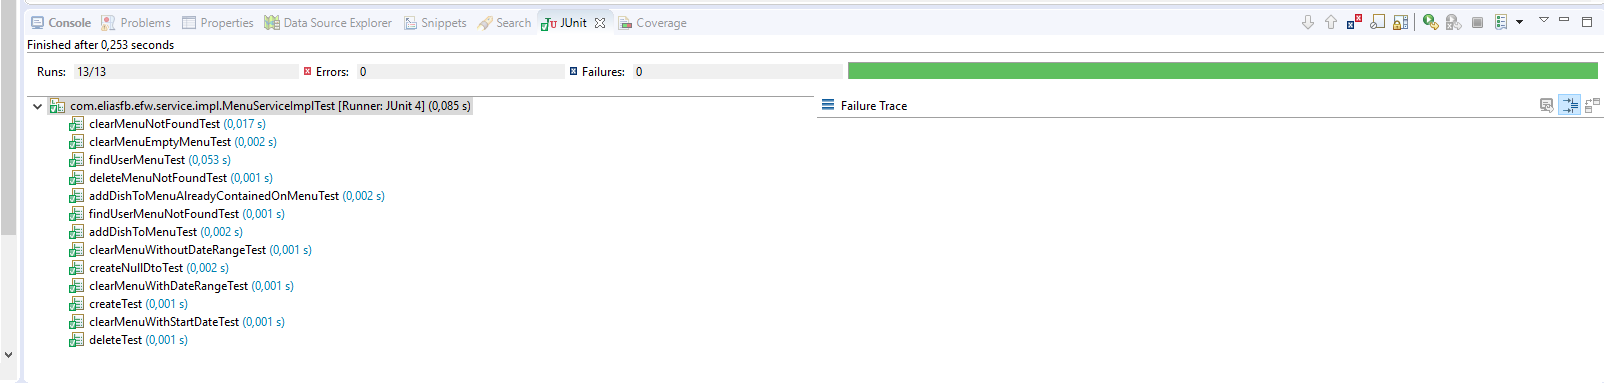
\includegraphics[width=15cm]{Imagenes/Tests.png}
		\caption{Tests Unitarios}\label{Tests Unitarios}
	\end{figure}
	\section{Cobertura}
	Utilizamos el plugin de Eclipse, Eclemma, para analizar el nivel de cobertura obtenido con las pruebas unitarias.
	Como se puede ver en la figura, el nivel de cobertura obtenido es bastante alto en la mayoría de los casos ya que, durante el desarrollo de las pruebas unitarias, nos hemos centrado en el recorrido de todas las posibles ramas del código, llamando a las operaciones con argumentos de todos los rangos de valores posibles.
	\begin{figure}[H]
		\centering
		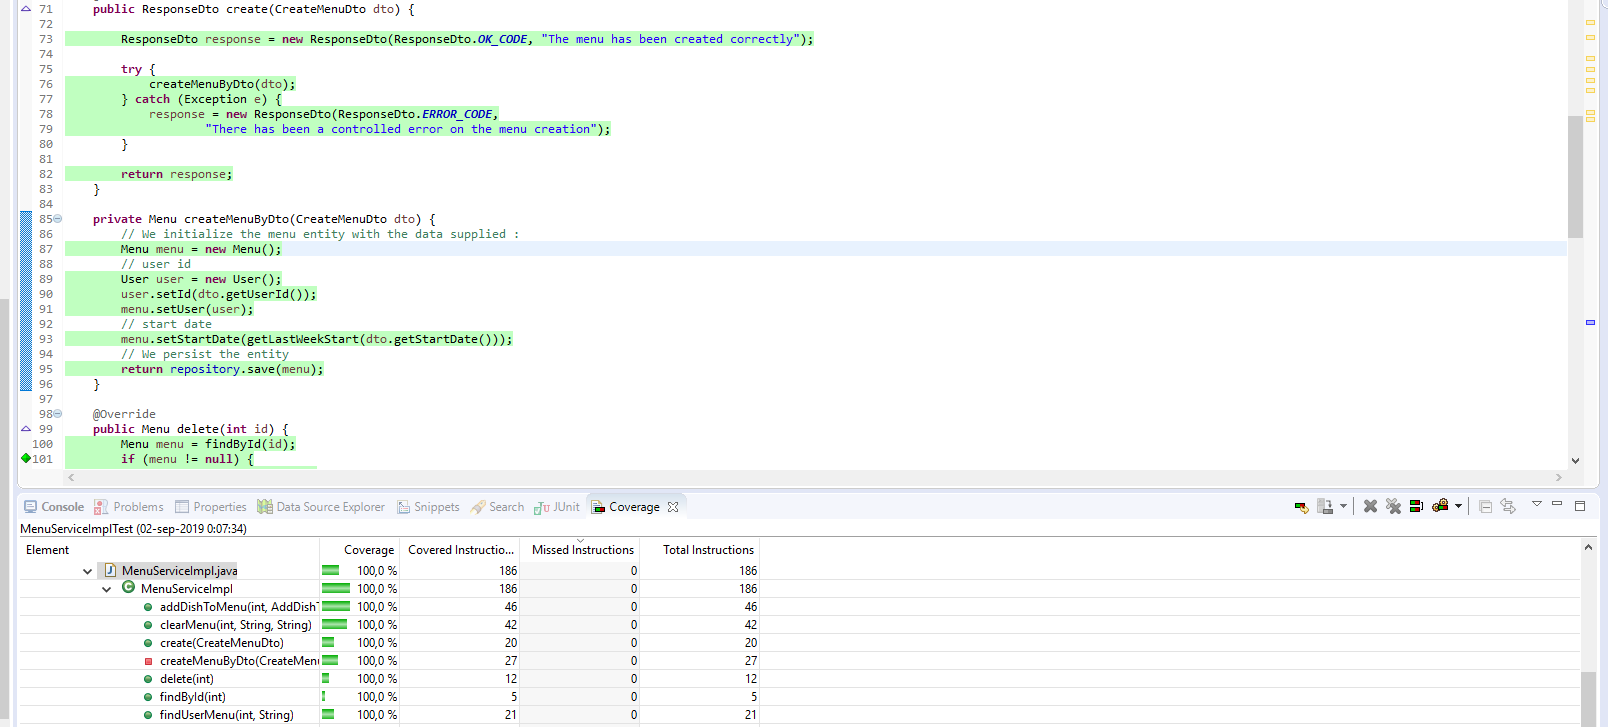
\includegraphics[width=15cm]{Imagenes/Cobertura.png}
		\caption{Cobertura}\label{Cobertura}
	\end{figure}
	\section{Pruebas Automáticas de Interfaz}
	Utilizamos puppeteer para automatizar las pruebas manuales de interfaz de forma que probamos tanto el funcionamiento del frontal como el del backend eliminando la tediosidad y lentitud de este tipo de pruebas manuales.\\
	Con puppeteer podemos crear un navegador y progrmar las acciones que realizaría el usuario para que se hagan automáticamente una detrás de otra con rapidez.\\
	\subsection{Generación automática de lista de la compra}
	Como ejemplo de script de Puppeteer tenemos el acceso al sistema con un usuario de prueba y la generación de la lista de la compra de su menú actual en el momento del acceso a la visión de menú.\\
	Para hacer estos pasos automáticamente creamos el siguiente script JS y delegamos en Node para que lo ejecute:
	\begin{lstlisting}
		const puppeteer = require('puppeteer');
		function delay(time) {
			return new Promise(function(resolve) {
				setTimeout(resolve, time)
			});
		}
		async function main() {
			const browser = await puppeteer.launch({ignoreHTTPSErrors: true, headless: false});
			const page = await browser.newPage();
			await page.setViewport({width: 1200, height: 720})
			await page.goto('https://localhost:4200/users/login', { waitUntil: 'networkidle0' }); // wait until page load
			await page.type('#email', 'test@mail.com');
			await page.type('#password', '1234');
			// click and wait for navigation
			await Promise.all([
				page.click('#loginButton'),
				page.waitForNavigation({ waitUntil: 'networkidle0' })
			]);
			await delay(1000);
			page.click('#shoppingListButton');
			await delay(1000);
			await page.screenshot({path: 'shoppingList.png'});
		}
		
		main();		
	\end{lstlisting}
	La ejecución de este script realiza los siguientes pasos:
	\begin{itemize}
		\item Acceder a la página de login de nuestro sistema
		\item Introducir un usuario y una contraseña correctos y loggearse haciendo click en el botón de confirmación
		\item El sistema con el inicio de sesión navega automáticamente a la visualización semanal del menú
		\item Esperamos 1 segundo a que se cargue el menú actual y todo el formulario correspondiente
		\item Hacemos click en "Shopping List" para obtener la lista de la compra
		\item Esperamos 1 segundo a que se genere el pop up con la lista de la compra
		\item Sacamos una captura de pantalla con el resultado de todos estos pasos y la guardamos en shoppingList.png
	\end{itemize}
	En este script concreto hemos delegado la validación en una captura de pantalla que podemos revisar para asegurar que el funcionamiento ha sido el correcto: Se ha accedido a la visión semanal del usuario autenticado, se ha generado el pop up de la lista de la compra correctamente y sus datos son veraces.\\
	Sin embargo en este caso concreto también hemos dejado el navegador automático abierto con lo que tenemos la flexibilidad de revisarlo nosotros mismos o hacer más pruebas manuales sobre ese navegador.\\
	La captura de pantalla que obtenemos de la ejecución del script es la siguiente:
	\begin{figure}[H]
		\centering
		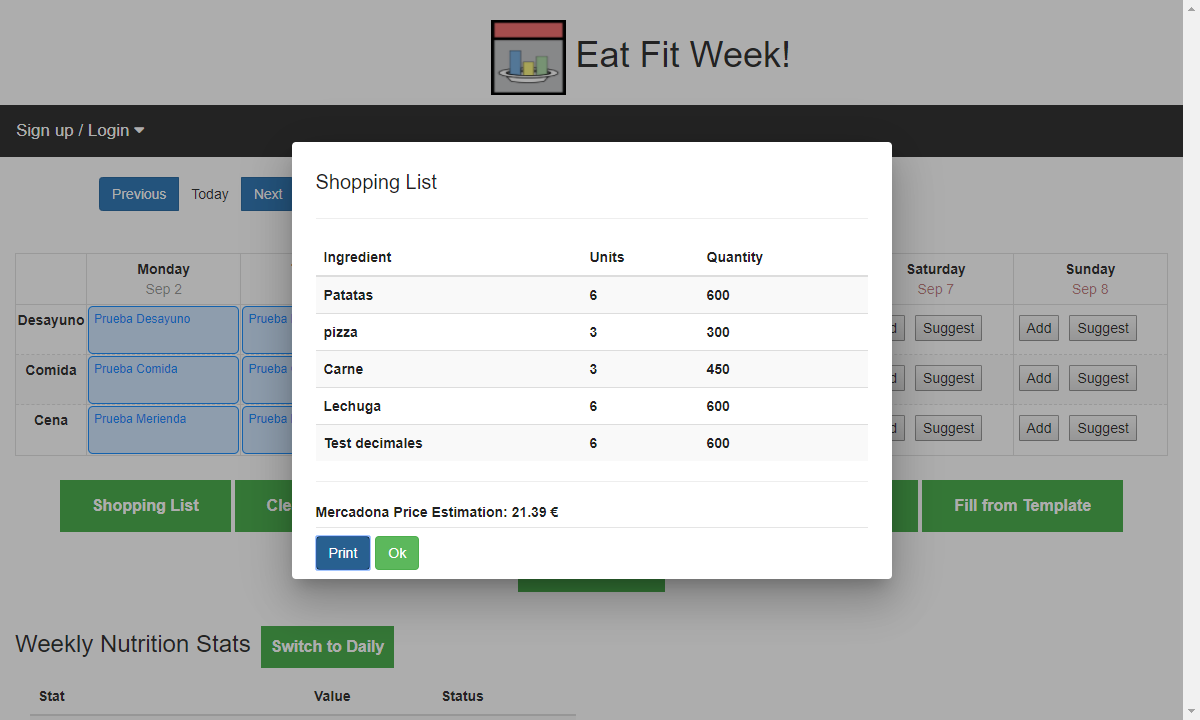
\includegraphics[width=15cm]{Imagenes/shoppingList.png}
		\caption{Shopping List ScreenShot}\label{Shopping List ScreenShot}
	\end{figure}
	\section{Pruebas de Usuario}
	El ser un sistema de gran aplicabilidad y tener un público tan variado nos ha permitido organizar sesiones de prueba y feedback con potenciales usuarios en diferentes etapas del desarrollo del sistema.
	Esto nos ha dado dos ventajas:
	\begin{itemize}
		\item Pruebas de integración de backend y frontend sobre el sistema en usos habituales del sistema
		\item Obtención de nuevos requisitos no concebidos en la planificación inicial. Requisitos a mayores obtenidos de estas sesiones han sido: Hacer las comidas semanales configurables (Desayuno, Comida, Merienda ...) tanto su número como sus nombres y Añadición de plato a primer hueco disponible de menú permitido
	\end{itemize}
	Estas pruebas a mayores añaden verificación de calidad sobre el sistema en un uso ``real'' de la aplicación. 
	Para estas pruebas se han realizado los siguientes pasos para cubrir los casos de uso de la aplicación desde un usuario totalmente nuevo:
	\begin{itemize}
		\item Registrar un nuevo usuario en el sistema
		\item Loggearse con ese usuario recién creado
		\item Registrar ingredientes habituales en la dieta de la persona que está haciendo estas pruebas de usuario
		\item Formar platos con los ingredientes registrados
		\item Configurar valores máximos de stats nutricionales semanales coherentes con la dieta que sigue la persona que hace las pruebas
		\item Planificar los platos creados en el menú de la semana en la que se está accediendo
		\item Ejecutar acciones sobre este menú: Obtener su lista de la compra, Mover sus platos a diferentes huecos, Borrar el menú, Regenerarlo automáticamente y válidamente
		\item Dejar que el sistema le sugiera platos en diferentes huecos en función de sus platos registrados hasta el momento
	\end{itemize}
	Durante todas estas pruebas hemos hecho énfasis en detectar posibles malas experiencias de usuario durante el proceso normal de su uso del sistema desde que empieza a utilizarlo, como puede ser el registro de una gran cantidad de ingredientes en el principio del uso del sistema que se puede solucionar con una carga por defecto de ingredientes básicos en cada nuevo registro de usuario.
	\chapter{Conclusiones y futuras líneas de trabajo}
	\section{Conclusiones}
	La principal motivación de este proyecto consistía en tomar una idea ya ejecutada de forma similar en otros sistemas abordándolo desde otro punto, el énfasis en el seguimiento semanal / diario de los stats nutricionales, y haciendo un ejercicio de mejoría sobre ellos para evitar los errores más comunes de la mayoría, desarrollando un sistema que sea fácil de usar, requiera poco esfuerzo del usuario y resulta hasta entretenido, para evitar que se convierta en un ejercicio de monotonía y repetición, motivo principal por el que este tipo de sistemas dejan de ser usados por el usuario y lo captan durante poco tiempo.	
	Tras el desarrollo del proyecto se ha obtenido un sistema open-source con las siguientes funcionalidades:
	\begin{itemize}
		\item Gestión de ingredientes y platos: Creación, actualización, borrado y listado.
		\item Planificación semanal de menús como combinación de platos y seguimiento cercano de sus valores nutricionales revisando contra unos límites que puede imponer el usuario.
		\item Aprendizaje automático de las costumbres del usuario para permitir predecir los platos que querrá incorporar en sus siguientes menús. Llevado a cabo con la ayuda de la herramienta Open Source Weka.
		\item Integración con la red social Facebook para iniciar sesión en el sistema y para hacer comparticiones de menús en el perfil del usuario conectado
		\item Estimación del precio de las listas de la compra de los menús mediante un scrappeador Python que consulta el catálogo de la página web de Mercadona.
	\end{itemize}
	Se ha dado soporte a la internacionalización del sistema con tres idiomas principales: inglés, español y gallego.\\
	En el diseño de la interfaz del sistema hemos hecho énfasis en que sea multidispositivo, manteniendo tres vistas principales: WebStandard pensada para grandes pantallas como las de un ordenador de escritorio, WebTablet para dispositivos con pantallas más pequeñas pero de aún así buen tamaño y WebMobile para dispositivos móviles que se caracterizan por una pequeña pantalla.\\
	Hemos dedicado esfuerzo a la usabilidad de la aplicación para mejorar en todo momento la experiencia de usuario y evitarle trabajos repetitivos que se puedan automatizar. Todo este esfuerzo tiene efecto positivo sobre la accesibilidad del mismo verificando en este punto que se pueden acceder a todos los elementos del teclado utilizando únicamente el teclado en la versión Standard del sistema.\\
	En el diseño, arquitectura y desarrollo del sistema se ha trabajado en que sea de fácil cambio y mantenibilidad con lo que futuras funcionalidades sean triviales de añadir y no incurran en riesgo.\\
	Se han tomado decisiones tecnológicas y de implementación para facilitar la escalabilidad del sistema mejorando la eficiencia de nuestras consultas y utilizando spring que, entre sus módulos tiene spring cloud, que proporciona utilidades de escalabilidad. Al no disponer de tareas programadas nuestro servidor es near-stateless con lo que se podrá ejecutar en N instancias.\\
	Para desarrollar con éxito este proyecto, hemos requerido de la aplicación directa de muchos de los conocimientos adquiridos a lo largo del máster, especialmente de las asignaturas orientadas al desarrollo de software, diseño, recuperación de la información e inteligencia de negocio asi como las de planificación y aseguramiento de calidad.\\
	Podemos afirmar que la elección de tecnologías fue la acertada ya que facilitó en gran medida el desarrollo del proyecto sobre todo gracias al conocimiento previo ya adquirido. Hemos conseguido una toma de contacto sobre una tecnología antes no conocida como es Angular JS, lo cual con un poco de trabajo adicional puede suponer una nueva aptitud profesional para el mercado laboral.
	\section{Futuras Líneas de Trabajo}
	\subsection{Integración Continua}
	Para automatizar el aseguramiento de la calidad en cada nuevo desarrollo software sería conveniente configurar un proceso de Integración Continua. 
	Para ello, en proyectos open source alojados en Github se tienen estas tres principales alternativas: Travis CI, Jenkins y Semaphore CI.
	Travis CI es un servicio de integración continua alojado que se utiliza para construir y probar proyectos de software alojados en GitHub. Los proyectos de código abierto como el nuestro se pueden probar sin cargo a través de travis-ci.org
	\subsection{Aplicaciones nativas móviles}
	Esta mejoría sobre el sistema no es exagerademente crucial al haberse adaptado la interfaz del mismo y su funcionamiento para poder adaptarse a diferentes pantallas entre las cuales se encuentra la de una pantalla móvil.
	Pese a ello, las aplicaciones nativas móviles tienen la ventaja de poder aprovechar mejor los recursos propios del teléfono como la vibración, cámara, acelerómetro. Al publicarla en la Play Store también se ganaría en divulgación y una mayor cantidad de potenciales usuarios llegarían a saber del sistema.
	A mayores, estas aplicaciones pueden ser más eficientes al estar pensadas para ejecutarse sobre el firmware de un teléfono móvil y pueden tener diseños mejor pensados para estas pantallas.
	Como facilidad para esta futura línea de trabajo, el patrón MVC facilita la elaboración de un nuevo cliente ya que, salvo en caso de nueva funcionalidad únicamente aplicable al nuevo cliente, no se necesitaría ningún cambio sobre el modelo o la capa REST y solo se necesitaría el esfuerzo necesario para capa frontal móvil.
	\subsection{Colecciones globales}
	Dentro de la política del ahorro del trabajo inicial que debe hacer cada nuevo usuario para empezar a planificar sus menús una nueva funcionalidad de mucho valor para el cliente sería la opción de visualizar ingredientes, platos y menús de cualquier usuario en lugar de únicamente los suyos propios. Al acceder a esas entidades de otros usuarios podríamos indicar un botón "Clonar" que le permitiera copiarla dentro de su repertorio. De esta forma, los usuarios podrían ver un plato que les guste que ha registrado otro usuario y clonarlo para empezar a usarlo de inmediato en sus menús sin tener que pasar por el trabajo de añadir todos los ingredientes que componen el plato y añadir posteriormente el plato.
	Esta funcionalidad mejoraría el carácter social del sistema y podría dar pie a interacciones entre los usuarios y los motivaría a registrar platos y menús de calidad para que resultaran atractivos a otros potenciales usuarios que puedan querer clonarlos en sus repertorios. Sería interesante valorar la opción de hacer platos/menús/ingredientes privados para el posible caso de que el usuario pueda no querer compartir con el resto algunos en concreto. Se debería valorar si es marca de privacidad tendría sentido hacerla a nivel de usuario o a nivel de entidad concreta.
	Se podría crear una nueva petición POST en el backend con el formato: '/efw-back/dishes/dishId/clone' a la que se le envie el json:
	\{\\
		``userId'':user id of the user that wants to clone the dish\\
	\}\\
	El servicio debería crear un nuevo plato con los datos del id de plato indicado y registrarlo en los platos del usuario indicado. Se debería crear una petición similar con los ingredientes. Desde la interfaz se podría crear una visualización similar a la de la visualización de platos e ingredientes del usuario conectado. En esas tablas globales se debería visualizar el usuario al que pertenecen los platos / ingredientes. Debería poder filtrarse de alguna forma para ayudar en la búsqueda de resultados concretos.
	\subsection{Fotos de platos}
	Permitir añadir fotos a cada uno de los platos registrados por el usuario mejoraría radicalmente su visualización y nos permitiría mostrar en la visión semanal del menú su foto en lugar de su nombre lo cual nos daría una visión global del menú de un mero vistazo sin tener que pararnos a revisar los nombres de cada uno de los platos en él.
	Una foto sacada con buena presentación sobre un plato puede motivar más al usuario y hacer el plato más apetecible lo cual puede asegurar que se cumpla mejor la dieta establecida en caso de estar el usuario siguiendo una.
	Para el almacenamiento de las diferentes fotos de los platos se debería intentar analizar las diferentes alternativas. Las principales serían: almacenar las imágenes en un servicio de cloud como puede ser Amazon Simple Storage Service(S3), esta solución puede tener el problema de encarecerse a la que los usuarios aumenten y el número de fotos por lo tanto aumente. La otra principal opción sería almacenar el fichero de alguna forma en nuestro modelo MySql con una columna BLOB o similar y hacerselo llegar al frontal a través de nuestra API.
	\subsection{Ingredientes ignorados en la lista de la compra}
	Una posible mejora sobre la gestión de ingredientes y la generación de la lista de la compra de cada menú es añadir esta marca sobre cada ingrediente de forma que, ingredientes que el usuario puede tener acumulados en casa y no precise comprar de forma habitual como pueden ser aceite, sal, arroz o pasta(En caso de que tenga la costumbre de comprar grandes cantidades de estos dos ingredientes poco perecederos).
	Evitar que estos ingredientes sean incluidos en las listas de la compra puede ayudar al usuario a liberarse de ruido en las listas que obtenga del sistema y pueda tener una estimación más real del precio de los alimentos que realmente va a comprar. A su vez puede hacer algo más eficiente el proceso de generación y estimación de la lista de la compra si se filtran estos ingredientes desde el principio de los cálculos.
	Para la marca booleana de aquellos ingredientes que no se tengan en cuenta en la lista de la compra podemos utilizar el patrón decorador para esta funcionalidad opcional sobre la entidad.
	\begin{thebibliography}{99}
		\bibitem{Scrum}
		Alan Cyment,
		\emph{El espíritu de Scrum: El arte de amar los lunes}
		\bibitem{Nutrition}
		Gene Stone y Michael Greger
		\emph{How Not to Die}
		\bibitem{Analysis}		
		Mauro Pezze,
		\emph{Software Testing and Analysis: Process, Principles and Techniques}
		\bibitem{Design}
		Kent Beck y Martin Fowler,
		\emph{Refactoring},
		1999
		\bibitem{Domain Driven Design}
		Eric Evans,
		\emph{Domain-Driven Design: Tackling Complexity in the Heart of Software}
		\bibitem{Software Architecture}
		Len Bass, Rick Kazman, Paul Clements
		\emph{Software Architecture in Practice}
		\bibitem{Patrones}
		Erich Gamma,
		\emph{Patrones de diseño},
		Addison Wesley, Massachusetts,
		1ra edición,
		2002.\\
		Addy Osmani,
		\emph{Learning JavaScript Design Patterns},
		2012.\\
		Murat Yener y Alex Theedom,
		\emph{Profesional Java EE Design Patterns},
		2014
		\bibitem{Java}
		Benjamin Aumaille,
		\emph{J2EE - Desarrollo de aplicaciones Web},
		ENI, Massachusetts,
		1ra edición,
		2012.
	\end{thebibliography}
	\renewcommand{\bibname}{Enlaces de interés}
	\begin{thebibliography}{99}
		\bibitem{Spring}
		Spring, \url{http://projects.spring.io/spring-framework/\#documentation}
		\bibitem{Spring Image}
		Spring Image,
		\url{http://doc.javanb.com/spring-framework-reference-zh-2-0-5/images/spring-overview.png}
		\bibitem{Eclipse Foundation}
		Eclipse Foundation, \url{http://www.eclipse.org/home/newcomers.php}
		\bibitem{Git}
		Git, \url{https://git-scm.com/}
		\bibitem{Git Image}
		Git Image, \url{http://www.pihomeserver.fr/wp-content/uploads/2015/05/raspberry-pi-git-server.jpg}
		\bibitem{HTML}
		HTML, \url{http://www.desarrolloweb.com/manuales/manual-html.html}
		\bibitem{CSS}
		CSS, \url{http://librosweb.es/libro/css/capitulo\_1.html}
		\bibitem{TexStudio}
		TexStudio, \url{http://www.texstudio.org/}
		\bibitem{Maven}
		Maven, \url{http://maven.apache.org/what-is-maven.html}
		\bibitem{JUnit}
		JUnit, \url{http://junit.org/junit4/}
		\bibitem{MySQL}
		MySQL, \url{http://www.mysql.com/products/community/}
		\bibitem{Latex}
		Latex, \url{https://www.latex-project.org/}
		\bibitem{UML}
		UML, \url{http://www.uml.org/what-is-uml.htm}
		\bibitem{Eclemma}
		Eclemma, \url{http://www.eclemma.org/}
		\bibitem{Inyeccion de dependencias}
		Inyeccion de dependencias, \url{http://desarrolloweb.com/articulos/patron-diseno-contenedor-dependencias.html}
		\bibitem{Patron Factoria}
		Patron Factoria, \url{http://tratandodeentenderlo.blogspot.com.es/2010/02/patrones-de-diseno-factorias.html}
		\bibitem{Mixins Component}
		Mixins Component,
		\url{http://tapestry.apache.org/component-mixins.html},
		\bibitem{Scrum}
		Scrum,
		\url{https://www.scrum.org/}
	\end{thebibliography}
	\chapter{Acrónimos}
	\textbf{AJAX} Asynchronous JavaScript And XML\\
	\textbf{API} Application Programming Interface\\
	\textbf{CSS} Cascading Style Sheets\\
	\textbf{HTML} HyperText Markup Language\\
	\textbf{HTTP} Hypertext Transfer Protocol\\
	\textbf{HTTPS} Hypertext Transfer Protocol Secure\\
	\textbf{IDE} Integrated Development Environment\\
	\textbf{JSON} JavaScript Object Notation\\
	\textbf{MVC} Model–View–Controller\\
	\textbf{MVP} Minimum Viable Product\\
	\textbf{ORM} Object-Relational Mapping\\
	\textbf{PDF} Portable Document Format\\
	\textbf{POM} Project Object Model\\
	\textbf{REST} Representational State Transfer\\
	\textbf{UML} Unified Modeling Language\\
	\textbf{URL} Uniform Resource Locator\\
	\textbf{XML} eXtensible Markup Language\\
	\textbf{XSD} XML Schema Definition
	\appendix
	\chapter{Apéndice}
	\section{Manual de Usuario}
	En esta sección se explicará el manejo de la aplicación web desarrollada.
	\subsection{Autenticación}
	Al presionarse el botón de Iniciar sesión se mostrará su formulario en el que se solicitará el email y la contraseña del usuario que quiere autenticarse en el sistema. \\
	Al confirmar, en caso de haberse indicado datos correctos se redigirá automáticamente a la visión semanal del menú del usuario. En caso de datos incorrectos, se indicará que ha habido un error en el inicio de sesión.\\
	Se permite también iniciar sesión con una cuenta de Facebook del usuario.
	\begin{figure}[H]
		\centering
		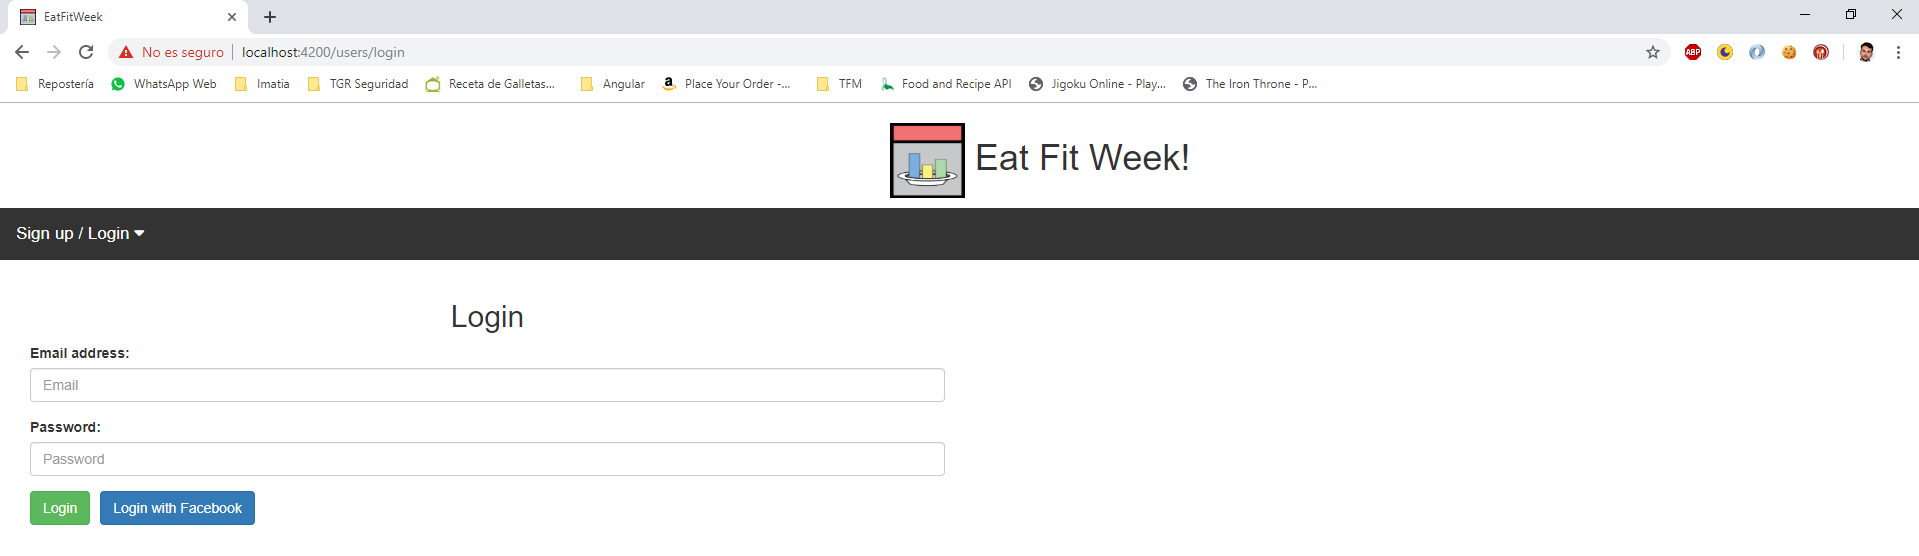
\includegraphics[width=15cm]{Imagenes/MU-Login.png}
		\caption{Log in}\label{Log in}
	\end{figure}
	\subsection{Registro}
	Al presionar en el botón de Registro se muestra el formulario en el que se solicitan los datos necesarios para dar de alta un nuevo usuario: Email, nombre, apellidos y contraseña.\\
	En caso de indicarse datos correctos y confirmar, se creará una nueva cuenta para el usuario y se le redirigirá a la pantalla de inicio de sesión para que pueda autenticarse con la cuenta recién creada.
	\begin{figure}[H]
		\centering
		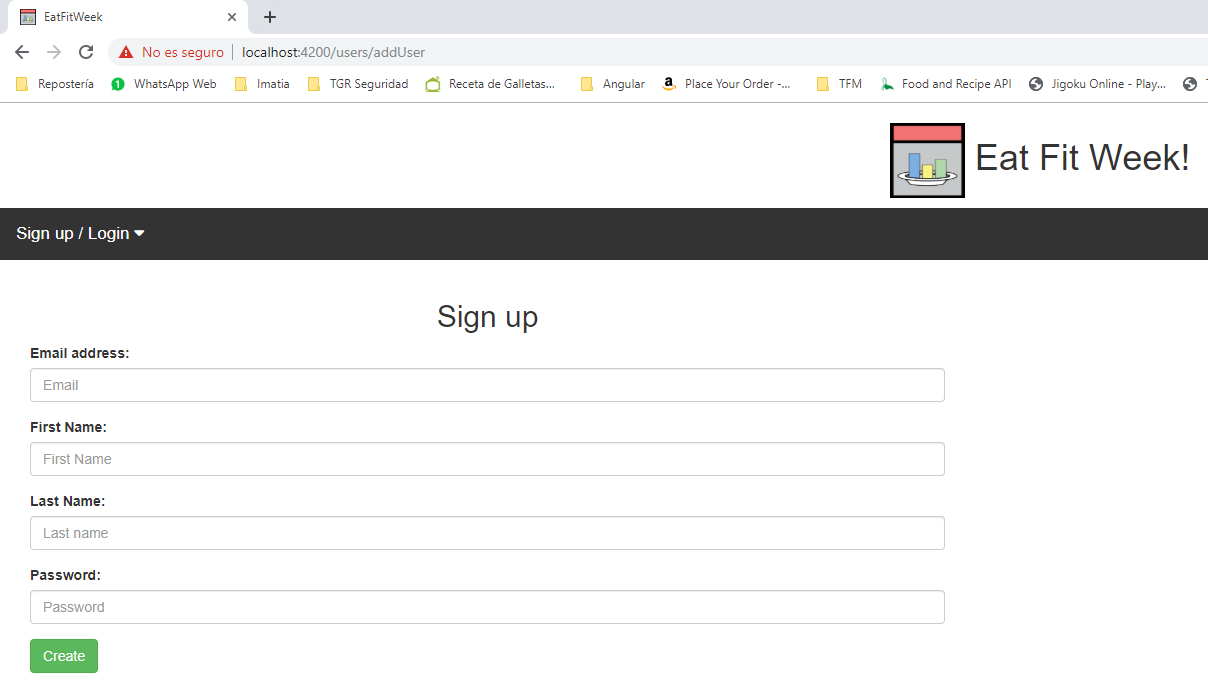
\includegraphics[width=15cm]{Imagenes/MU-Registro.png}
		\caption{Sign up}\label{Sign up}
	\end{figure}
	\subsection{Añadir ingrediente}
	Una vez autenticado, se permite al usuario acceder al resto de funcionalidades de la aplicación. Entre ellas, se encuentra el formulario de añadir ingrediente.\\
	En este formulario se le solicita al usuario: nombre del ingrediente que quiere registrar, su categoría alimenticia y sus stats nutricionales(Calorías, Proteinas, Grasas y Carbohidratos). Una vez rellenado el nombre del ingrediente se le permite al usuario intentar estimar automáticamente los stats nutricionales del ingrediente pulsando en el botón de estimación.
	\begin{figure}[H]
		\centering
		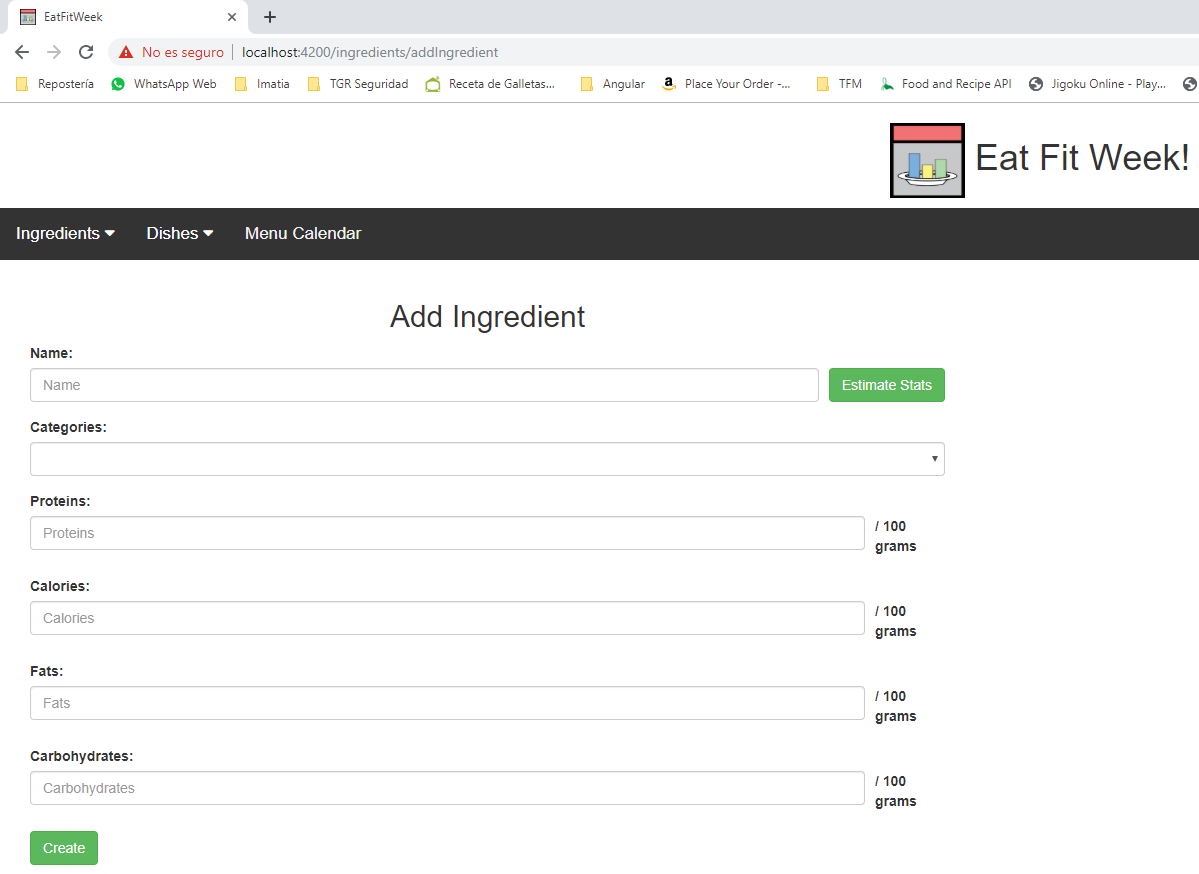
\includegraphics[width=15cm]{Imagenes/MU-AddIngredient.png}
		\caption{Add ingredient}\label{Add ingredient}
	\end{figure}
	\begin{figure}[H]
		\centering
		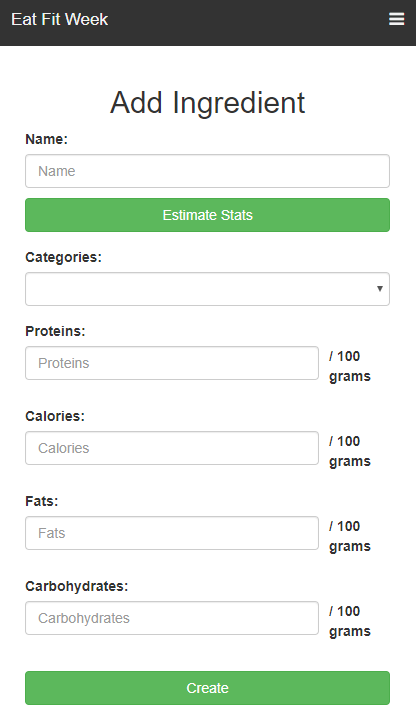
\includegraphics[width=10cm]{Imagenes/MU-AddIngredientMobileTablet.png}
		\caption{Add ingredient Mobile And Tablet}\label{Add ingredient Mobile And Tablet}
	\end{figure}
	\subsection{Listado ingredientes}
	Al seleccionar en el menú ``Listado de ingredientes'' se le permite ver al usuario todos sus ingredientes registrados y, para cada uno de ellos, se visualiza: su nombre, su categoría alimenticia y sus stats nutricionales.\\ También se muestra un warning en caso de que el ingrediente pertenezca a una categoría de las prohibidas por el usuario. Por último, se permite para cada ingrediente acceder a su formulario de actualización o bien borrarlo.\\
	En la versión tablet no se muestra el warning por el escaso espacio en el diseño y en la versión mobile solo se muestran las calorías de los stats nutricionales al ser el stat más relevante.
	\begin{figure}[H]
		\centering
		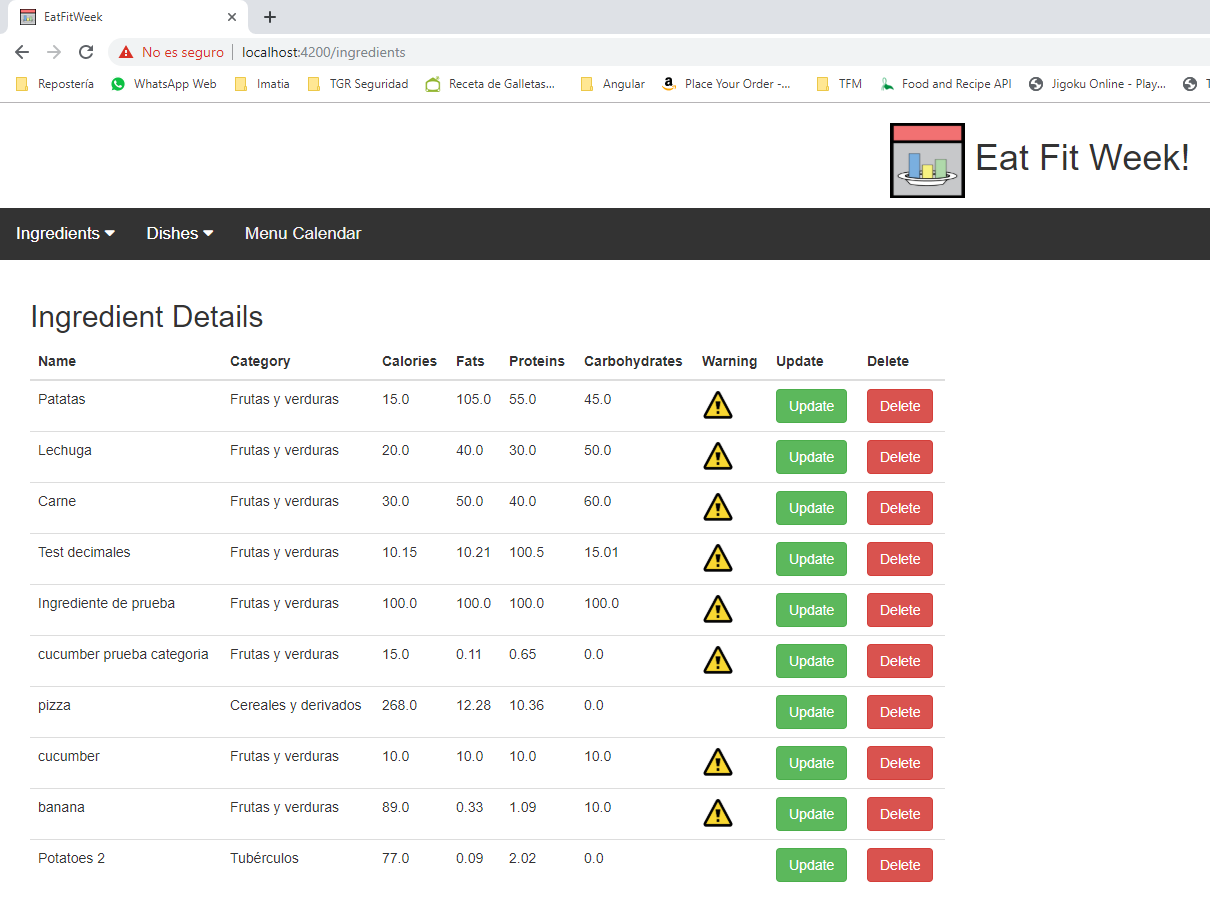
\includegraphics[width=15cm]{Imagenes/MU-ListIngredients.png}
		\caption{List ingredients}\label{List ingredients}
	\end{figure}
	\begin{figure}[H]
		\centering
		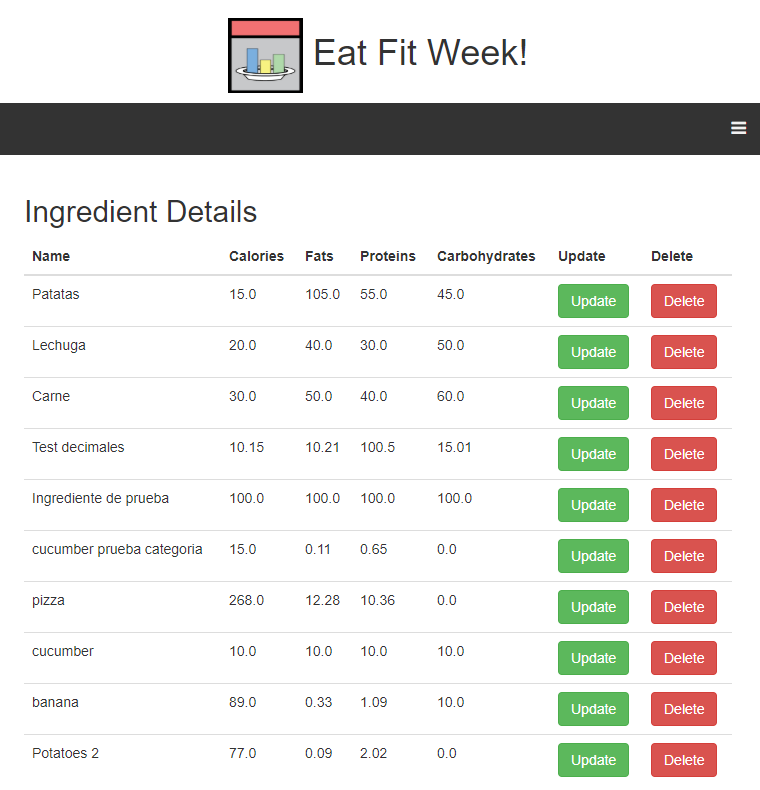
\includegraphics[width=15cm]{Imagenes/MU-ListIngredientsTablet.png}
		\caption{List ingredients Tablet}\label{List ingredients Tablet}
	\end{figure}
	\begin{figure}[H]
		\centering
		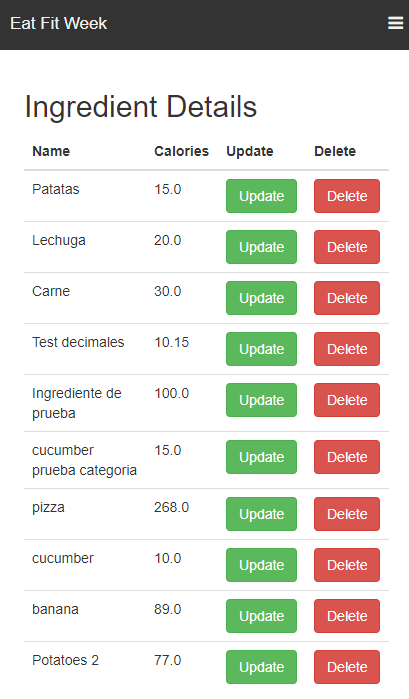
\includegraphics[width=10cm]{Imagenes/MU-ListIngredientsMobile.png}
		\caption{List ingredients Mobile}\label{List ingredients Mobile}
	\end{figure}
	\subsection{Actualización ingrediente}
	Al seleccionar el botón ``Actualizar'' en una de las filas del listado de ingredientes se accede al formulario de actulización de ingrediente. Presenta los mismos campos y misma funcionalidad que el formulario de añadir ingrediente pero se utiliza únicamente sobre ingredientes ya dados de alta y está inicializado con los datos del ingrediente.	
	\begin{figure}[H]
		\centering
		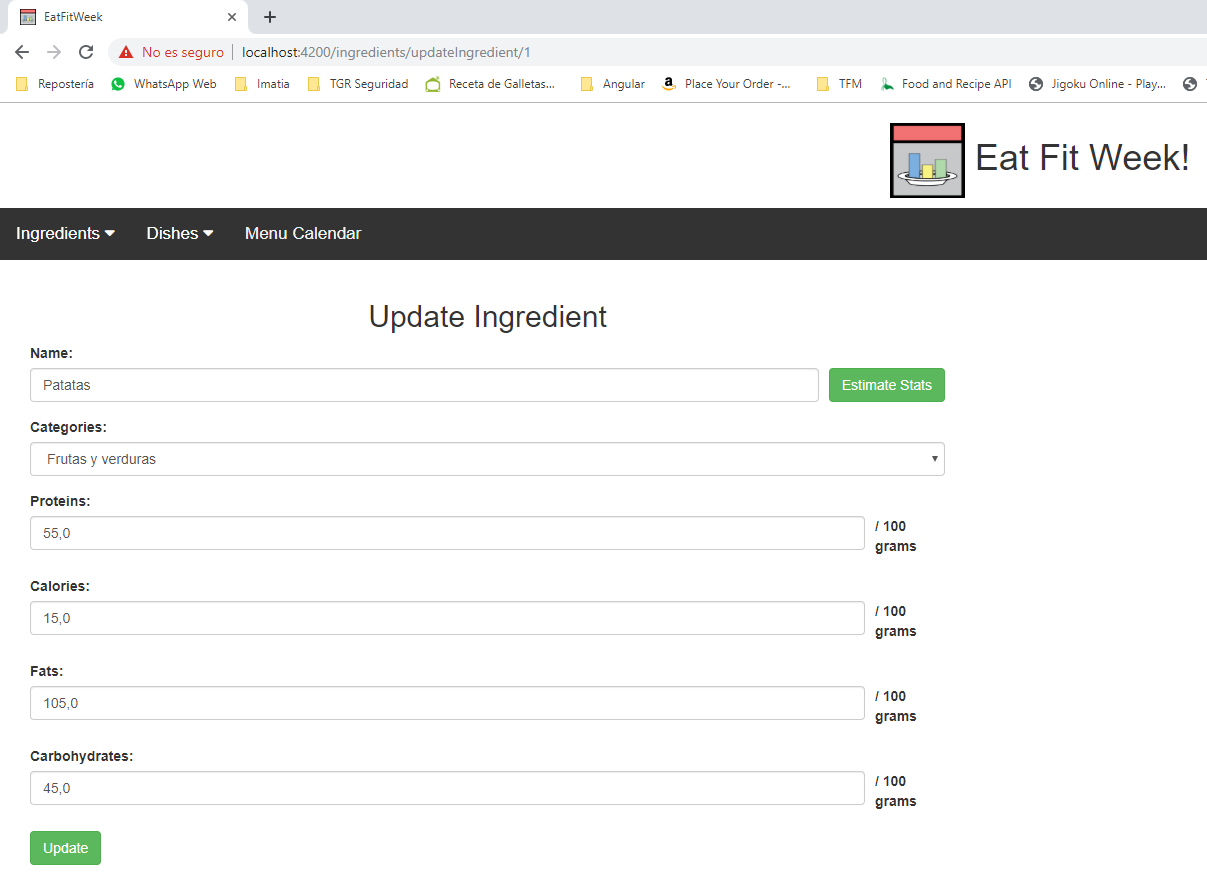
\includegraphics[width=15cm]{Imagenes/MU-UpdateIngredient.png}
		\caption{Update ingredient}\label{Update ingredient}
	\end{figure}
	\begin{figure}[H]
		\centering
		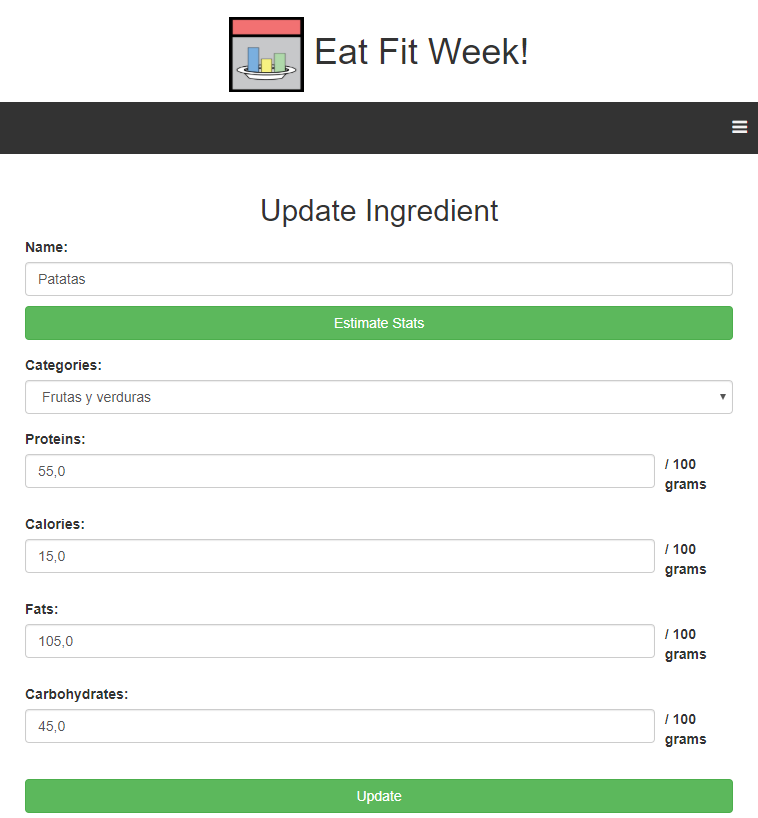
\includegraphics[width=15cm]{Imagenes/MU-UpdateIngredientMobileTablet.png}
		\caption{Update ingredient Mobile Tablet}\label{Update ingredient Mobile And Tablet}
	\end{figure}
	\subsection{Añadir plato}
	Al seleccionar en el menú ``Añadir plato'' se permite acceder a su formulario, en él se le solicita al usuario: los ingredientes que componen el plato y para cada uno de ellos la cantidad del ingrediente en el plato, se le solicita la receta de elaboración del plato, las comidas en las que estará permitido el plato (Inicialmente se permite en todas) y por último el nombre del plato.
	Una vez añadido un ingrediente, se mostrarán tanto los ingredientes que tiene el plato seleccionados como sus stats nutricionales. El campo del nombre del plato tiene un mecanismo de auto rellenado para facilitar la labor del usuario: Con el primer ingrediente seleccionado, se establece como nombre del plato y los siguientes ingredientes seleccionados se añaden al nombre mediante conjunciones, por ejemplo: en caso de seleccionar tres ingredientes en este orden, Carne, Patatas y Lechuga; el nombre del plato se iniciará a ``Carne con Patatas y Lechuga''. De todas formas en todo momento se permite al usuario editar ese nombre por si quiere editarlo o elegir uno propio.
	\begin{figure}[H]
		\centering
		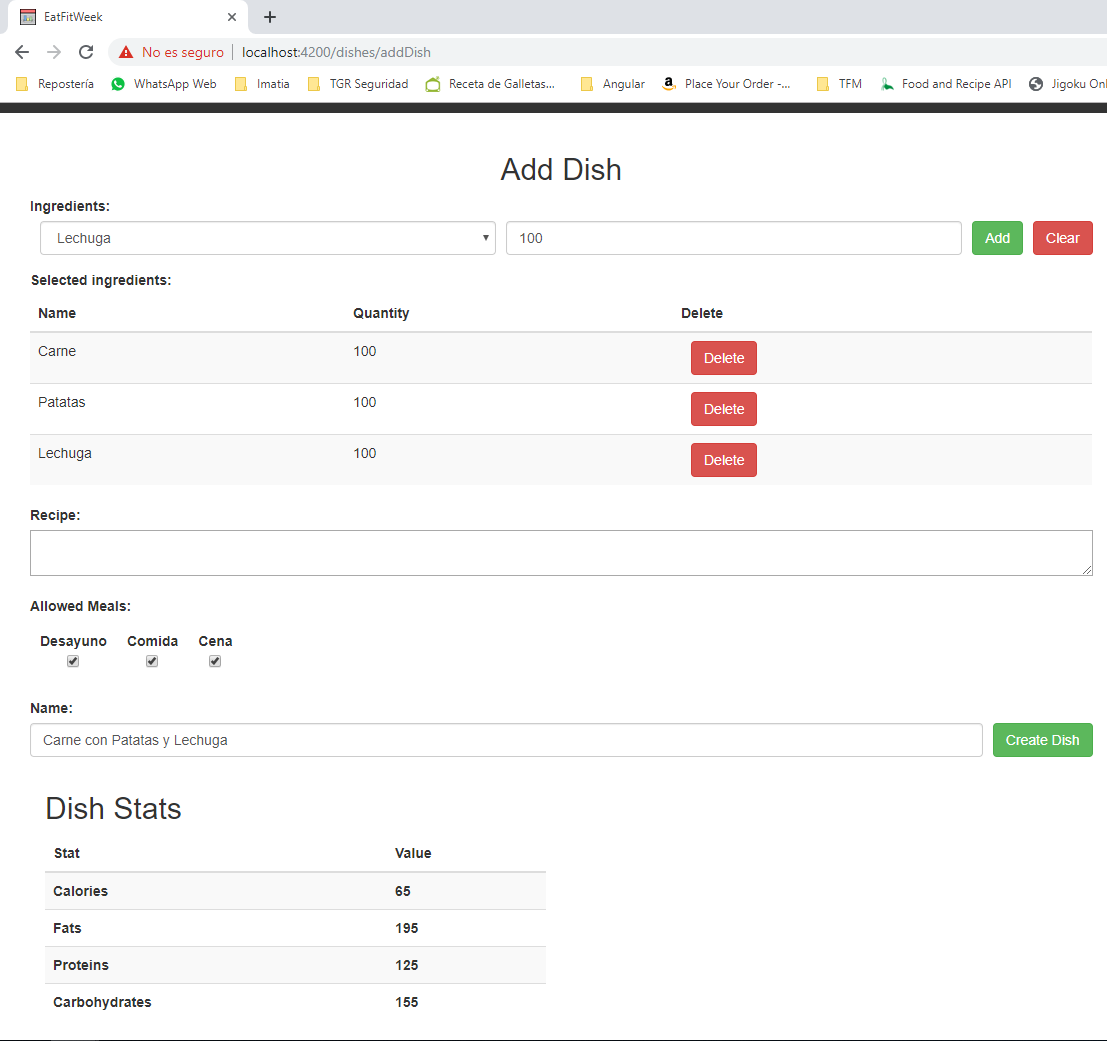
\includegraphics[width=15cm]{Imagenes/MU-AddDish.png}
		\caption{Add dish}\label{Add dish}
	\end{figure}
	\begin{figure}[H]
		\centering
		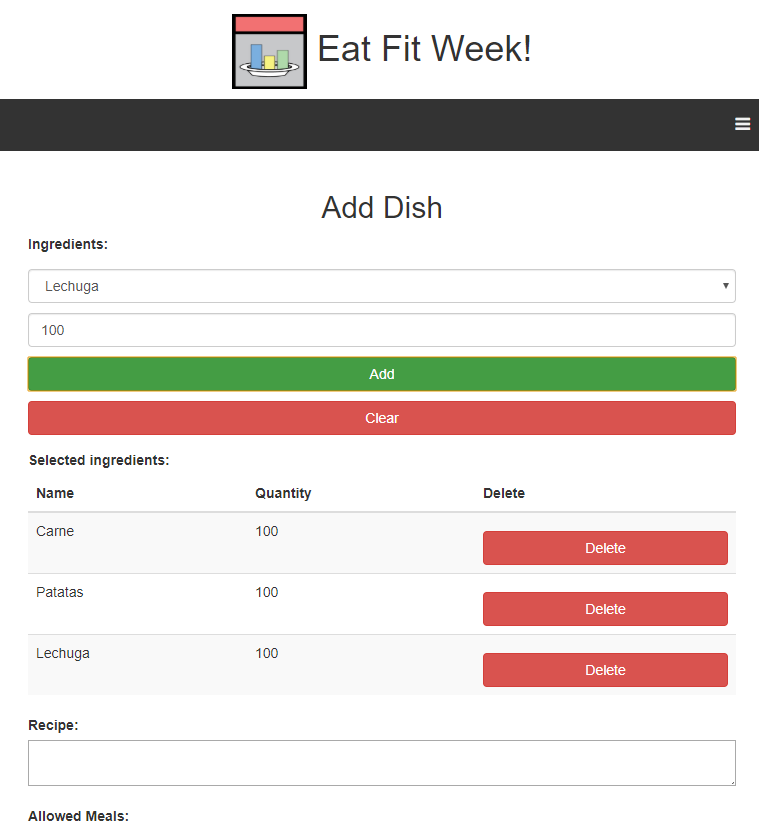
\includegraphics[width=15cm]{Imagenes/MU-AddDishMobileTablet.png}
		\caption{Add dish Mobile And Tablet}\label{Add dish Mobile And Tablet}
	\end{figure}
	\subsection{Listado de platos}
	Al seleccionar en el menú ``Listado de platos'' se accederá a su formulario en el que se visualizarán todos los platos registrados por el usuario. Para cada uno de ellos se visualizarán los siguientes datos: nombre y stats nutricionales. También se permitirá acceder a su actualización, borrar el plato o bien añadirlo al menú actual en el primer hueco válido para el plato.\\
	En la versión tablet no se muestra la opción de añadir el plato al menú actual ya que no tiene tanto sentido al no verse toda la semana en el mismo formulario y poder confundir al usuario y en la versión mobile solo se muestran las calorías de los stats nutricionales al ser el stat más relevante y tener escaso espacio en el diseño.
	\begin{figure}[H]
		\centering
		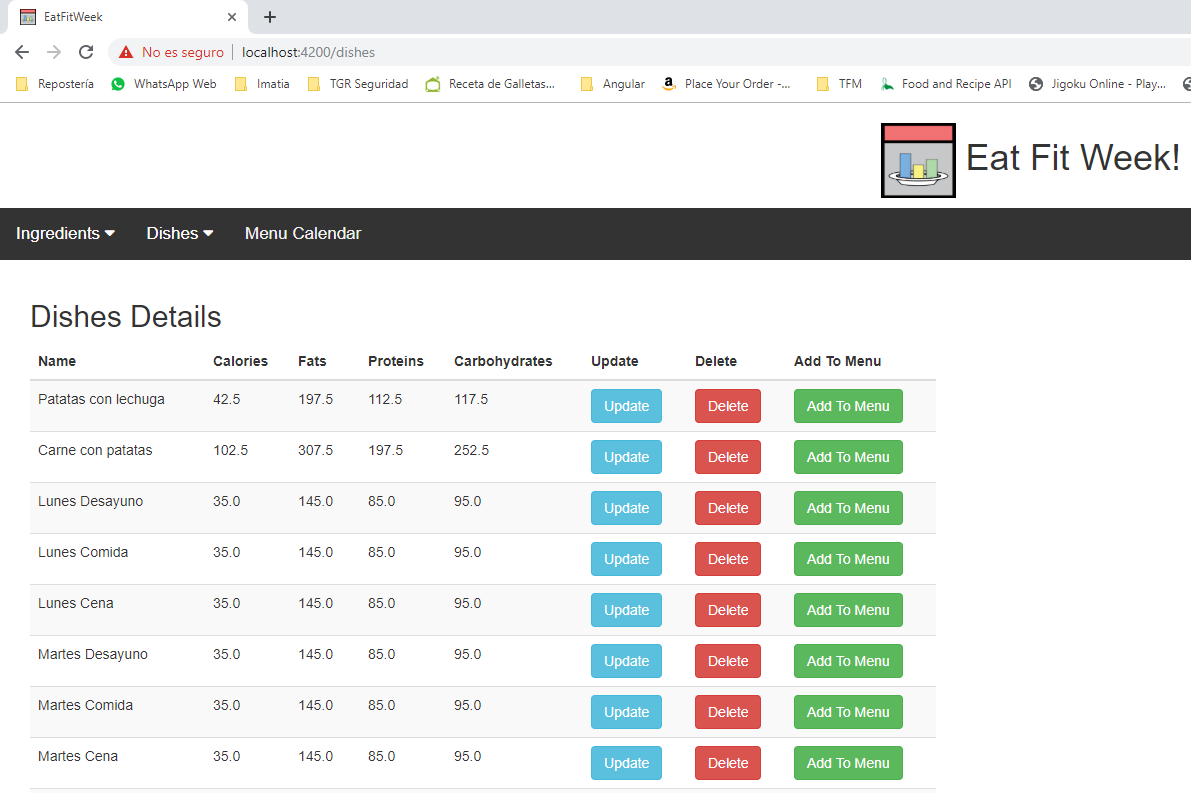
\includegraphics[width=15cm]{Imagenes/MU-ListDishes.png}
		\caption{List dishes}\label{List dishes}
	\end{figure}
	\begin{figure}[H]
		\centering
		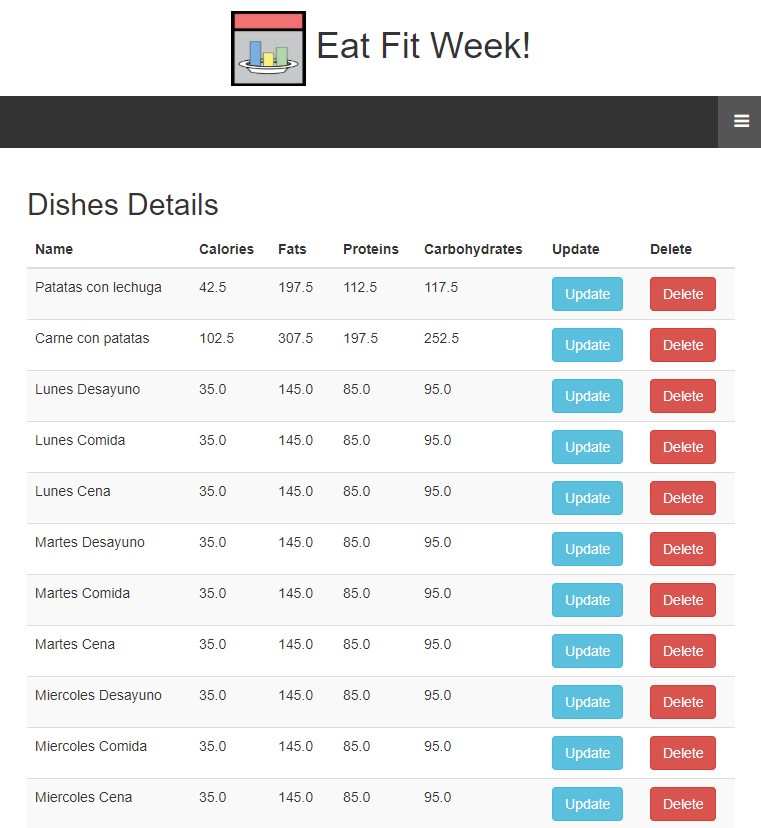
\includegraphics[width=15cm]{Imagenes/MU-ListDishesTablet.png}
		\caption{List dishes Tablet}\label{List dishes Tablet}
	\end{figure}
	\begin{figure}[H]
		\centering
		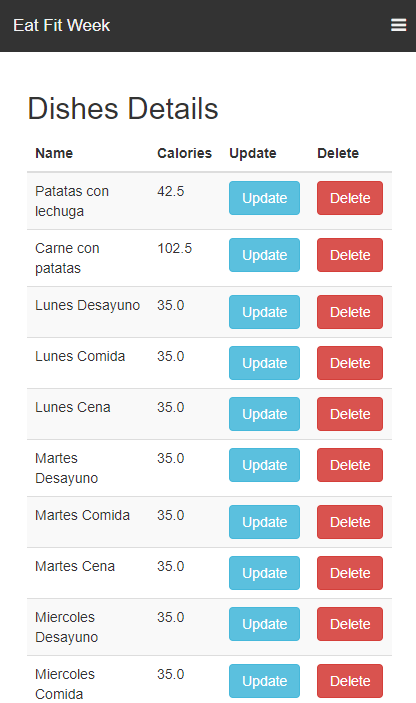
\includegraphics[width=10cm]{Imagenes/MU-ListDishesMobile.png}
		\caption{List dishes Mobile}\label{List dishes Mobile}
	\end{figure}
	\subsection{Actualización de plato}
	Al seleccionar el botón ``Actualizar'' en cada fila de la tabla de visualización de platos, se permitirá acceder al formulario de actualización de platos. Tiene el mismo funcionamiento y visualización que el formulario de añadir platos salvo por el hecho de que sólo se puede acceder a él en platos ya registrados y sus datos se inicializan con la información del plato.
	\begin{figure}[H]
		\centering
		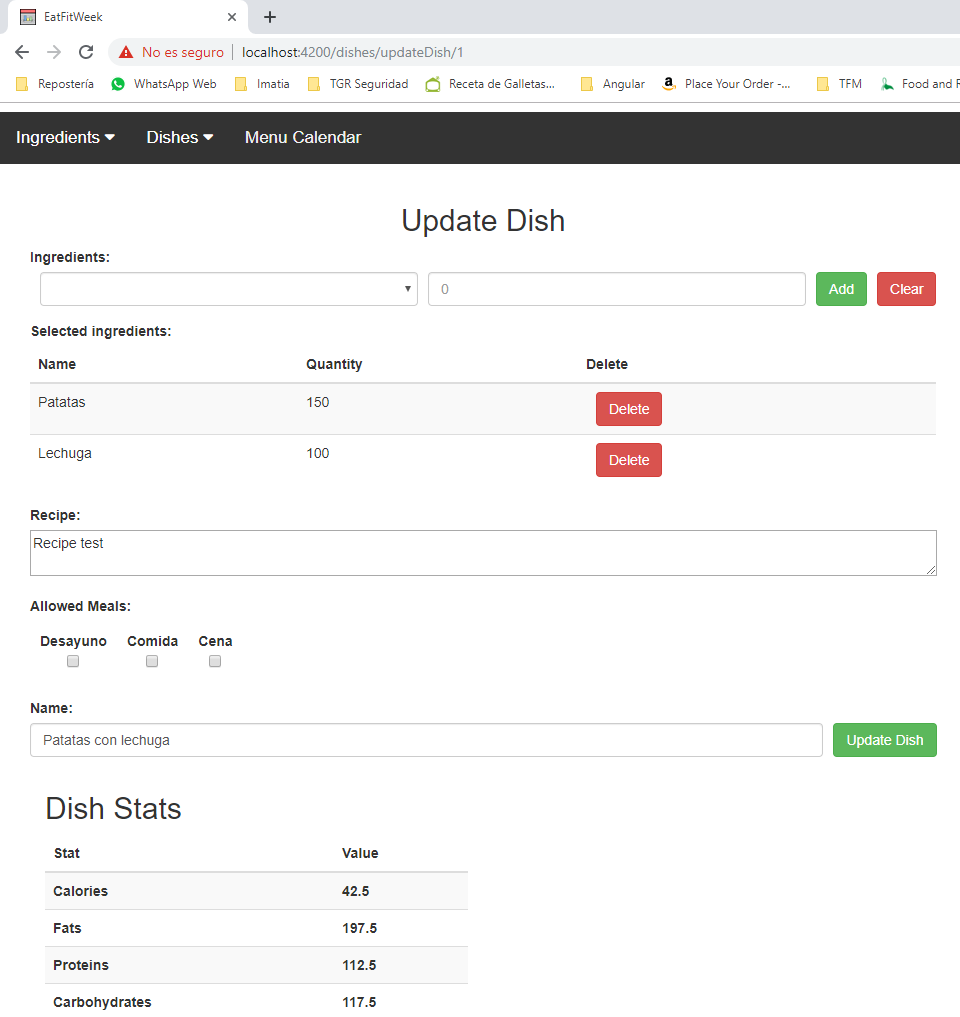
\includegraphics[width=15cm]{Imagenes/MU-UpdateDish.png}
		\caption{Update dish}\label{Update dish}
	\end{figure}
	\begin{figure}[H]
		\centering
		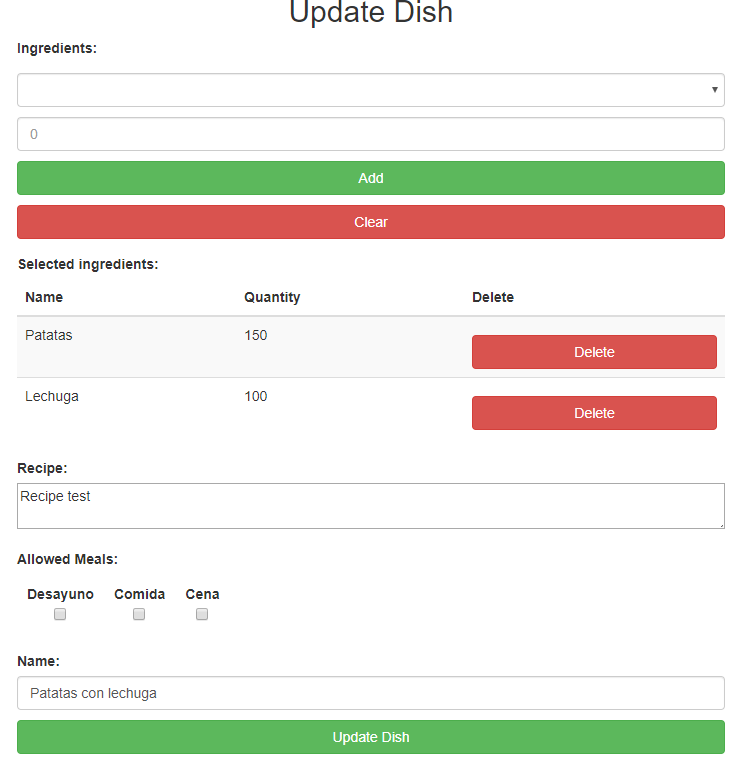
\includegraphics[width=15cm]{Imagenes/MU-UpdateDishMobileTablet.png}
		\caption{Update dish Mobile And Tablet}\label{Update dish Mobile And Tablet}
	\end{figure}
	\subsection{Configuraciones de usuario}
	Al seleccionar ``Configuraciones'' en el menú de usuario conectado se puede acceder a este formulario en el que se permite al usuario configurar el funcionamiento del sistema.\\
	Las configuraciones soportadas son: los valores máximos semanales de los stats nutricionales de los menús, las categorías alimenticias prohibidas por el usuario y las comidas semanales del usuario, tanto su número como su nombre.
	\begin{figure}[H]
		\centering
		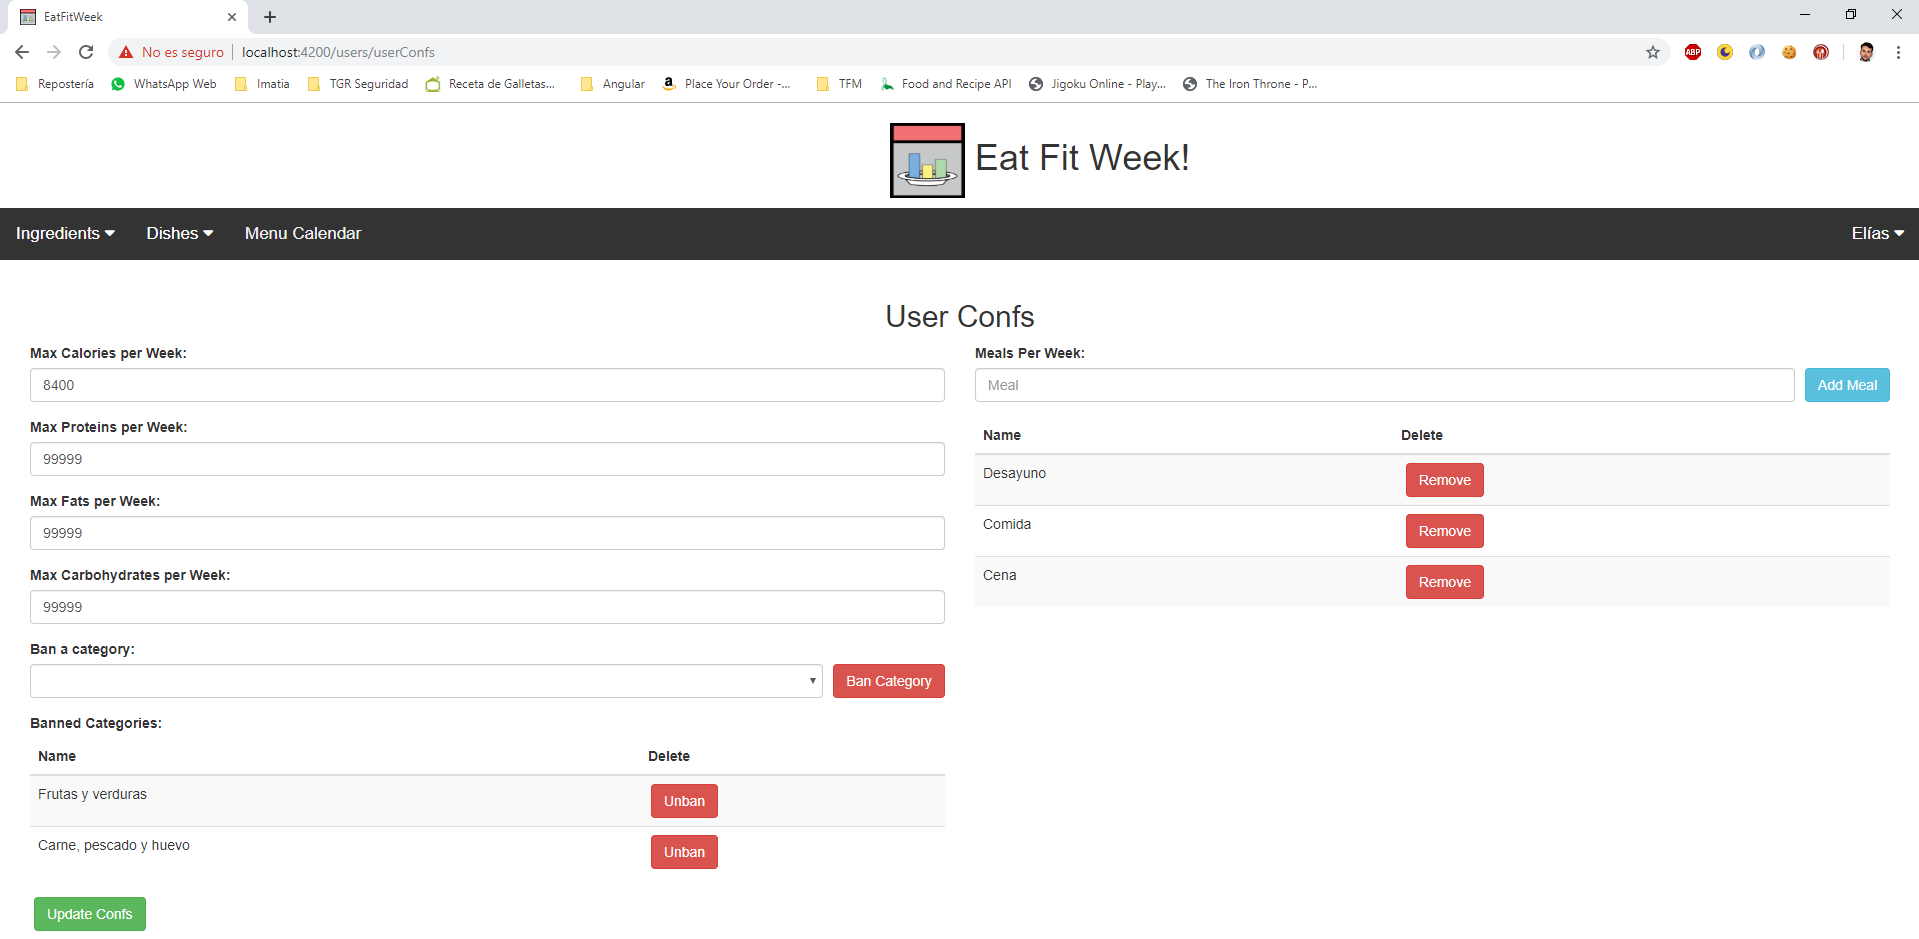
\includegraphics[width=15cm]{Imagenes/MU-UserConfs.png}
		\caption{User configurations}\label{User configurations}
	\end{figure}
	\begin{figure}[H]
		\centering
		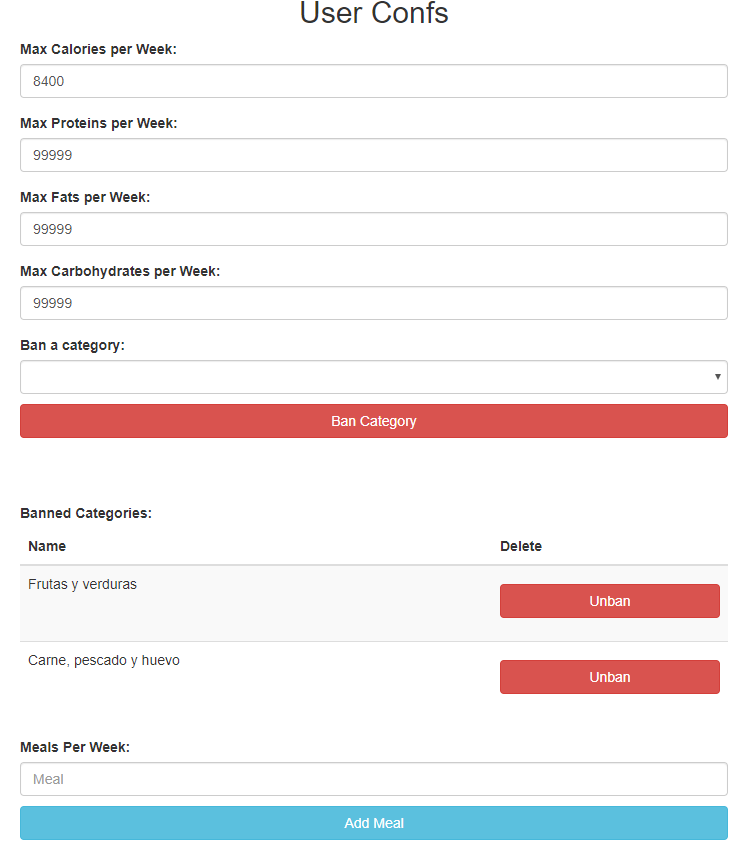
\includegraphics[width=15cm]{Imagenes/MU-UserConfsMobileTablet.png}
		\caption{User configurations Mobile And Tablet}\label{User configurations Mobile And Tablet}
	\end{figure}
	\subsection{Visualización semanal de los menús}
	Al seleccionar ``Calendario de Menú'' en el menú se accede a este formulario que representa la funcionalidad principal del sistema.\\
	Se muestra un grid con cada día de la semana como columnas y con las comidas como filas. Dentro de cada celda del grid, pueden ocurrir dos cosas:
	\begin{itemize}
		\item Que exista un plato planificado para ese hueco concreto del menú actual con lo que se visualizará su nombre. En caso de que el usuario haga click sobre ese hueco, se eliminará el plato del menú. En caso de que se mantenga pulsado ``Shift'' cuando se hace click sobre el plato, se replicará el plato en el menú de forma que se añadirá el mismo plato al siguiente hueco disponible permitido por el plato.
		\item Que no exista un plato para ese hueco concreto del menú actual con lo que se visualizarán dos botones: Uno para añadir un plato de entre los registrados por el usuario en ese hueco seleccionado y otro para  que el sistema sugiera al usuario un plato para ese hueco concreto.
	\end{itemize}
	Inicialmente se mostrará el menú que se corresponda con la semana en la que el usuario está accediendo al sistema pero se le permite desplazarse por semanas anteriores o siguientes sin límite.\\
	Se muestran también los stats nutricionales sumados de todos los platos del menú y se permite modificar la visualización para que se pueda cambiar a visualización diaria y se pueda seleccionar el día concreto del que se quiera visualizar sus stats. En caso de estar visualizándose los stats semanales se mostrará una marca que indique al usuario si se cumple con sus limites semanales o si se están infringiendo.\\
	Para todos los menús se visualizan una serie de acciones posibles, de izquierda a derecha: mostrar su lista de la compra, eliminar los platos del menú, rellenar el menú con platos aleatorios, rellenar el menú con platos que no violen los límites nutricionales del usuario, guardar los platos del menú como una plantilla para cargar en otros menús, rellenar el menú con los platos de una plantilla previamente guardada por el usuario y por último imprimir el menú.
	En la visión tablet se visualizan tres días de cada vez en lugar del menú entero y en la visión mobile se visualiza un día de cada vez.\\
	En estas dos visiones se puede hacer scroll al siguiente tramo o al anterior mediante swipe hacia la izquierda y hacia la derecha respectivamente. Al llegar al final de la semana y hacer swipe hacia la izquierda se visualiza un formulario en el que se ve el resumen del menú semanal, , y se ofrecen las mismas acciones sobre el menú que en la versión standard.
	\begin{figure}[H]
		\centering
		\includegraphics[width=15cm]{Imagenes/MU-MenuView.png}
		\caption{Menu View}\label{Menu View}
	\end{figure}
	\begin{figure}[H]
		\centering
		\includegraphics[width=15cm]{Imagenes/MU-MenuViewTablet.png}
		\caption{Menu View Tablet}\label{Menu View Tablet}
	\end{figure}
	\begin{figure}[H]
		\centering
		\includegraphics[width=10cm]{Imagenes/MU-MenuViewMobile.png}
		\caption{Menu View Mobile}\label{Menu View Mobile}
	\end{figure}
	\begin{figure}[H]
		\centering
		\includegraphics[width=15cm]{Imagenes/MU-MenuWeekViewMobileTablet.png}
		\caption{Menu Week View Mobile And Tablet}\label{Menu Week View Mobile And Tablet}
	\end{figure}
\end{document}
